\documentclass[a4paper,11pt,twoside]{report}

\overfullrule=5pt % draw overfull hboxes for visual inspection

\usepackage[
	%showframe, % show frame for page margins etc.
	scale=0.75, % fraction of page width/height to use
	headheight=30pt,
	%marginpar=2cm, % define to avoid \marginpar{} from overflowing
]{geometry}
\newcommand\TODO[1]{\textcolor{red}{(\textbf{TODO:} #1)}}
\newcommand\TODOM[1]{\marginpar{\TODO{#1}}}

\usepackage{ifdraft}
%\usepackage[utf8]{inputenc} % ignored with lualatex / xelatex (which are utf8-based)
\usepackage{amsmath}
\usepackage{dsfont} % for identity operator \mathds{1}
\usepackage{mathtools}
\usepackage{tensor}
\usepackage{braket}
\usepackage[retain-unity-mantissa = false]{siunitx}
\usepackage{slashed}
\usepackage[parfill]{parskip} % new paragraph: new line, no indent
%\usepackage[title]{appendix}
\usepackage[hidelinks]{hyperref} % hide colored boxes around links
\usepackage[noabbrev]{cleveref}
\usepackage{mdframed} % TODO: remove, only to draw frames for marking relevant sections to supervisor

\usepackage[labelfont=bf]{caption} % figure title in bold
\usepackage[labelfont=bf]{subcaption} % figure title in bold
%\captionsetup{subrefformat=parens}
\DeclareCaptionLabelFormat{bold}{\textbf{(#2)}}
\captionsetup{subrefformat=bold}

\usepackage{graphicx}
\usepackage[usetransparent=false,inkscapepath=.cachesvginkscape/]{svg}

%\usepackage{unicode-math} % make code display utf8 characters properly (seems that only fontspec below is enough?)
%\setmonofont{DejaVu Sans Mono} % will affect whole document, including URLs etc.
\usepackage{fontspec}
\newfontfamily\codefont{DejaVu Sans Mono}[NFSSFamily=CodeFamily] % set mono font for minted code only
\ifdraft{
	\usepackage{fancyvrb} % fast, but ugly
	\fvset{fontfamily=CodeFamily}
	\fvset{fontsize=\scriptsize}
	\fvset{frame=single}
	\newcommand{\codefile}[2]{\VerbatimInput{#2}}
}{
	\usepackage[cachedir=.cacheminted/]{minted} % nice, but slow
	%\setminted{breaklines}
	\setminted{frame=single}
	\setminted{breakanywhere}
	\setminted{fontfamily=CodeFamily}
	\setminted{fontsize=\scriptsize}
	\newcommand{\codefile}[2]{\inputminted{#1}{#2}}
}

\usepackage{fancyhdr}
\pagestyle{fancy}
\fancyhf{}
\fancyhead[LE,RO]{\textbf{\thepage}}
\fancyhead[RE]{\leftmark}
\fancyhead[LO]{\rightmark}
\fancyfoot[CE,CO]{}

\usepackage{tikz}
\usetikzlibrary{external}

% OLD. I did this before. But did not play well after adding -output-directory option.
% \tikzexternalize[prefix=.cachetikz/] % DO NOT USE DIRECTORY NAME WITH _ (. seems ok after changing .latexmkrc)

% NEW. Dirty fix for using -output-directory option. From https://tex.stackexchange.com/a/338560
\tikzexternalize
\tikzset{%
external/system call={xelatex \tikzexternalcheckshellescape --halt-on-error --interaction=batchmode --output-directory=./.cachelatex --jobname "\image" "\texsource"},
	/pgf/images/include external/.code={%
		\includegraphics{.cachelatex/#1}%
	},
}

\usepackage{pgfplots}
\usepackage{pgfplotstable}
% NOTE: externalization does NOT recompile when only the global options below are changed
\pgfplotsset{
	compat=1.17,
	% Using title={\subcaption{...}} REQUIRES text width to be set, otherwise it throws hard-to-understand errors
	% TODO: the contents of title={...} MUST change for the externalization library to recompile the figure
	every axis title/.style={at={(0.5,1)}, align=center, above=1ex, text width=0.8*\pgfkeysvalueof{/pgfplots/width}]},
}
\usepgfplotslibrary{groupplots}

\pgfplotsset{
	/pgfplots/colormap={parametrize}{rgb255=(255,255,0) rgb255=(255,0,0)}
}
\pgfplotsset{
	/pgfplots/colormap={blackred}{rgb255=(0,0,0) rgb255=(255,0,0)}
}
\pgfplotsset{
	/pgfplots/colormap={negpos}{rgb255=(0,0,255) rgb255=(0,0,0) rgb255=(255,0,0)}
}
\pgfplotsset{
	/pgfplots/colormap={stability}{rgb255=(0,255,0) rgb255=(255,0,0) rgb255=(128,0,0) rgb255=(0,0,0)}
}
\pgfplotsset{
	/pgfplots/colormap={plasma}{%
		rgb=(0.050383, 0.029803, 0.527975)
		rgb=(0.186213, 0.018803, 0.587228)
		rgb=(0.287076, 0.010855, 0.627295)
		rgb=(0.381047, 0.001814, 0.653068)
		rgb=(0.471457, 0.005678, 0.659897)
		rgb=(0.557243, 0.047331, 0.643443)
		rgb=(0.636008, 0.112092, 0.605205)
		rgb=(0.706178, 0.178437, 0.553657)
		rgb=(0.768090, 0.244817, 0.498465)
		rgb=(0.823132, 0.311261, 0.444806)
		rgb=(0.872303, 0.378774, 0.393355)
		rgb=(0.915471, 0.448807, 0.342890)
		rgb=(0.951344, 0.522850, 0.292275)
		rgb=(0.977856, 0.602051, 0.241387)
		rgb=(0.992541, 0.687030, 0.192170)
		rgb=(0.992505, 0.777967, 0.152855)
		rgb=(0.974443, 0.874622, 0.144061)
		%rgb=(0.940015, 0.975158, 0.131326) % hard to see yellow on white
	},
}
\pgfplotsset{
    /pgfplots/colormap={viridisrev}{
        indices of colormap={
            \pgfplotscolormaplastindexof{viridis},...,0 of viridis}
    },
    /pgfplots/colormap={plasmarev}{
        indices of colormap={
            \pgfplotscolormaplastindexof{plasma},...,0 of plasma}
    },
}

\newcommand{\tablemaximum}[5]{
	\pgfplotstableread{#1}{\mytable}
	\pgfplotstablesort[sort key=#2, sort cmp=float >]{\mytablesorted}{\mytable}
	\pgfplotstablegetelem{0}{#2}\of\mytablesorted
	\pgfmathsetmacro{#3}{\pgfplotsretval} % find the maximum
	\pgfplotstablegetelem{0}{#4}\of\mytablesorted
	\pgfmathsetmacro{#5}{\pgfplotsretval} % find an associated value
}

%\fancypagestyle{plain}{\pagestyle{fancy}} % make chapter front pages, bibliography etc. use same style as other pages (see https://tex.stackexchange.com/a/10046)

% make consistent style also on chapter first pages, bibliography etc.
\fancypagestyle{plain}{
	\fancyhf{}
	\fancyhead[LE,RO]{\textbf{\thepage}}
}

% urldate=long and dateabbrev=false for full date, language=british for getting 17th September 2001 format (in biblatex, without affecting rest of document)
\usepackage[style=alphabetic,giveninits=true,maxnames=10,block=ragged,date=iso,urldate=iso,seconds=true,language=british]{biblatex} 
\DeclareFieldFormat{pages}{%
	page \mkfirstpage{#1}% print first page only
}
\AtEveryBibitem{
	\clearfield{series}
	\clearlist{location}
	\clearfield{pagetotal} % useless to se total number of pages
}
\DeclareFieldFormat*{edition}{\mkbibparens{\mkbibordedition{#1} edition}}
\DeclareFieldFormat*{title}{\emph{#1}} % always italic (not the case for article titles by default)
\DeclareFieldFormat*{journaltitle}{#1} % no italics (in contrast to default)
\DeclareFieldFormat*{volume}{volume #1}
\newbibmacro*{journal+date}{
	\printtext{Published in}%
	\setunit*{\addspace}
	\mkbibbold{\printfield{year}}%
	\setunit*{\addspace}
	\printtext{by}%
	\setunit*{\addspace}
	\printfield{journaltitle}%
	\setunit*{\addcomma\space}
	\printfield{volume}%
	\setunit*{\addcomma\space}
	\printfield{pages}
}
\DeclareBibliographyDriver{article}{%
	\usebibmacro{begentry}%
	\usebibmacro{author+title+edition}%
	\newunit\newblock
	\usebibmacro{journal+date}%
	\newunit\newblock
	\usebibmacro{isbn+doi+url}%
	\usebibmacro{begentry}%
}
\renewbibmacro*{publisher+location+date}{%
	\printtext{Published in}%
	\setunit*{\addspace}%
	\mkbibbold{\printdate}%\printfield{year}%
	\setunit*{\addspace}%
	\printtext{by}%
	\setunit*{\addspace}%
	\printlist{publisher}%
}
\newbibmacro*{author+title+edition}{%
	\printnames{author}%
	\setunit*{\addcolon\space}%
	\printfield{title}%
	\iffieldundef{edition}{}{%
		\setunit*{\addspace}%
		\printfield{edition}%
	}%
	\newunit
}
\newbibmacro*{isbn+doi+url}{% ISBN -> DOI -> URL
	\iffieldundef{isbn}{%
		\iffieldundef{doi}{%
			\printfield{url}% do not have ISBN or DOI, so try to print URL (priority 3)
		}{%
			\printfield{doi}% do not have ISBN, but have DOI (priority 2)
		}%
	}{% 
		\printfield{isbn}% have ISBN (priority 1)
	}%
}
\DeclareBibliographyDriver{book}{%
	\usebibmacro{begentry}%
	\usebibmacro{author+title+edition}%
	\newunit\newblock
	\usebibmacro{publisher+location+date}%
	\newunit\newblock
	\usebibmacro{isbn+doi+url}%
	\usebibmacro{finentry}%
}

\DeclareFieldFormat*{urldate}{#1}
\newbibmacro*{published+viewed}{%
	\iffieldundef{year}{}{% print publication date if we have one
		\printtext{\autocap{p}ublished}%
		\setunit*{\addspace}
		\iffieldundef{day}{%
			\printtext{in}% YYYY       will follow
		}{%
			\printtext{on}% YYYY-MM-DD will follow
		}%
		\setunit*{\addspace}%
		\mkbibbold{\printdate}%\printfield{year}%
		\setunit*{\addcomma\space}% 
	}%
	\iffieldundef{urlyear}{}{% print download date if we have one
		\printtext{\autocap{d}ownloaded on}%
		\setunit*{\addspace}
		\printurldate%
	}
}
\DeclareBibliographyDriver{online}{%
	\usebibmacro{begentry}%
	\usebibmacro{author+title+edition}%
	\newunit\newblock
	\usebibmacro{published+viewed}%
	\newunit\newblock
	\printfield{url}%
	\usebibmacro{finentry}%
}

\addbibresource{project.bib}

\usepackage{derivative}
\derivset{\odv}[style-inf=\mathrm] % write normal derivatives with upright d
%\derivset{\odv}[switch-/=true]

\usepackage{bm}

\newcommand\dif{\mathop{}\!\mathrm{d}}
\newcommand{\abs}[1]{\left\lvert #1 \right\rvert}
\newcommand{\norm}[1]{\| {#1} \|} % TODO: remove?
\renewcommand{\det}[1]{\abs{#1}}
%\newcommand{\tdet}{\text{det}}
\DeclareMathOperator{\tdet}{det}
\DeclareMathOperator{\asin}{asin}
\DeclareMathOperator{\asinh}{asinh}
\DeclareMathOperator{\sgn}{sgn}
\newcommand{\integral}[4]{\int_{#3}^{#4} #1 \dif #2}
\newcommand{\variation}[1]{\delta #1}
\newcommand{\trace}[1]{\text{tr} #1}
\newcommand{\lagr}{\mathcal{L}}
\newcommand{\ham}{\mathcal{H}}
\newcommand{\numdensity}{\mathcal{N}}
\newcommand{\diag}[1]{\text{diag} \left( #1 \right)}
\newcommand{\taylor}{\simeq}
%\AtBeginDocument{\renewcommand{\vec}[1]{\mathbf{#1}}} % NB: need AtBeginDocument due to unicode-math: https://tex.stackexchange.com/a/457845
\renewcommand{\vec}[1]{{\bm{#1}}} % don't need AtBeginDocument now that I use fontspec instead of unicode-math
\newcommand{\bigo}{\mathcal{O}}
\newcommand\pathintdif{\mathcal{D}}
\newcommand{\pathint}[2]{\int \pathintdif #1 \, #2}
\newcommand{\comm}[2]{[ #1 , #2 ]}
\newcommand{\acomm}[2]{\{ #1 , #2 \}}
\newcommand{\thermalavg}[1]{ \left< #1 \right>}
\newcommand{\conj}[1]{{#1}^*}
%\newcommand{\res}{\text{Res}}
\DeclareMathOperator*{\res}{Res}
\DeclareMathOperator{\real}{Re}
\DeclareMathOperator{\imag}{Im}
\newcommand{\1}{\mathds{1}}
\newcommand{\diml}[1]{\hat{#1}} % use to denote dimensionless quantity
\newcommand{\solarmass}{M_\odot}

% useful intro to Latex thesis: https://www.overleaf.com/learn/latex/How_to_Write_a_Thesis_in_LaTeX_(Part_1):_Basic_Structure

\title{Neutron stars}
\author{Herman Sletmoen}
\date{\today}

\begin{document}

\maketitle
\tableofcontents
\chapter*{Notation and conventions} % do not number
\addcontentsline{toc}{chapter}{Notation and conventions} % but still display in TOC (see https://tex.stackexchange.com/a/222961)
%\markboth{NOTATION AND CONVENTIONS}{} % but still display correct header (see https://tex.stackexchange.com/a/78090)

\section*{Metric signature}

We use the $(+,-,-,-)$ metric signature.

\section*{Summation convention}

We use the Einstein summation convention, in which an index that appears once as a superscript and again as a subscript in the same term is to be summed over.
If the index is roman, the sum runs from $1$ to $3$, and if it is greek, it also runs over $0$.
For example,
\begin{equation*}
	T\indices{^\mu_\mu} = \sum_{\mu=0}^3 T\indices{^\mu_\mu}
	\quad \text{and} \quad
	T\indices{^i_i} = \sum_{i=1}^3 T\indices{^i_i}
	.
\end{equation*}

\iffalse
\section*{Fourier transformation}

We use the Fourier transformation convention
\begin{equation}
	f(k) = \int \dif x \, e^{i k x} f(x)
	\qquad \text{and} \qquad
	f(x) = \int \frac{\dif k}{2 \pi} \, e^{-i k x} f(k) .
\end{equation}
With this convention, the delta function $\delta(x' - x)$ is given by the highlighted part of
\begin{equation}
	f(x) = \int \frac{\dif k}{2 \pi} \, e^{-i k x} f(k)
	     = \int \dif x' \underbrace{\int \frac{\dif k}{2 \pi} \, e^{i k (x'-x)}}_{\displaystyle \delta(x'-x)} f(k) .
\label{eq:pre:delta_function}
\end{equation}
\fi

\TODO{big F in Figure, A in Appendix, etc?}

\chapter{Introduction}

\TODO{Recapitulate main points of project thesis:}

\TODO{some general intro about the possibility of quark stars}

In this chapter, we will study a hypothetical class of compact stars known as quark stars.
Let us summarize the main ingredients in this work.

\section{Tolman-Oppenheimer-Volkoff equation}

In \cref{chap:tov} we derived the Tolman-Oppenheimer-Volkoff equation
\begin{subequations}
\begin{align}
	\odv{P}{r} &= -\frac{G m \epsilon(P)}{r^2 c^2} \left( 1 + \frac{P}{\epsilon(P)} \right) \left( 1 + \frac{4 \pi r^3 P}{m c^2} \right) \left( 1 - \frac{2 G m}{r c^2} \right)^{-1} , \\
	\odv{m}{r} &= \frac{4 \pi r^2 \epsilon(P)}{c^2} .
\end{align}
\end{subequations}
It determines the pressure and mass gradients with relativistic corrections inside a spherically symmetric star composed of a perfect fluid in hydrostatic equilibrium.
Given the fluid's equation of state $\epsilon(P)$ that relates its pressure $P$ to its energy density $\epsilon$, it is a system of two equations for the two unknowns $P$ and $m$ and can be integrated.
We will seek mass-radius solutions to the equation, obtained by integrating it from the center $r=0$ with zero initial mass $m(0) = 0$ and some central pressure $P(0) = P_c$ until reaching the surface $r=R$ defined by a vanishing pressure $P(R) = 0$ and where the mass $m(R) = M$ defines the star's total mass.
By finding such solutions for a range of central pressures $P_c$, we parametrize a sequence of stars that we can plot in a mass-radius diagram.

\section{Thermal field theory}

To derive equations of state for quark matter, we will study quantum field theories whose dynamics is described by some Lagrangian density $\lagr$.
In \cref{chap:tft} we showed that the partition function in the grand canonical ensemble corresponding to a Lagrangian including both a fermionic field $\psi$ and a bosonic field $\phi$ is given by the path integral
\begin{equation}
	Z = \oint_- \pathintdif \bar{\psi} \oint_- \pathintdif \psi \oint_+ \pathintdif \phi \exp \Big\{ \int_0^\beta \dif \tau \int_V \dif^3 x \, \lagr_E[\bar{\psi}, \psi, \phi] \Big\} = e^{-\beta V \Omega} .
\end{equation}
Here $V$ is the spatial volume of the system, while its inverse temperature $\beta = 1/T$ define its ``temporal'' extent.
The sign subscripts on the closed integral signs is supposed to remind us of a property we showed extensively in \cref{chap:tft}: the bosonic fields must be periodic in inverse temperature time, while the fermionic fields must be anti-periodic.
If a symmetry of the Lagrangian admits a conserved Noether charge density $j^0$, we also saw that we could couple it to a chemical potential $\mu$ in the Lagrangian by including the term $\mu j^0$.
By computing (the logarithm of) the partition function, we have the grand potential $\Omega = -\log Z / \beta V$ from which we can calculate all thermodynamic quantities such as the (mean)
\TODO{this is already in $T=0$ form? write in general $T \geq 0$ form in this intro?}
\begin{equation}
	\text{density} \quad n = -\pdv{\Omega}{\mu}, \quad
	\text{pressure} \quad P = -\Omega, \quad
	\text{energy density} \quad \epsilon = -P + \sum_p \mu_p n_p .
\end{equation}
These expressions are valid in the approximation of zero temperature $T=0$ that we saw was valid for neutron stars in \cref{chap:nstars}.
As quark stars are expected to be ``more intense neutron stars'', we assume that this approximation still holds.

The equation of state $\epsilon(P)$ follows by eliminating the chemical potentials $\mu_p$ from the energy density $\epsilon(\mu_p)$ in favor of the pressure $P$.
In \cref{chap:nstars} we did so for pure neutron stars, for which there was only one chemical potential to eliminate.
Now we will study quark stars composed of up quarks, down quarks, strange quarks and electrons, each associated with their own chemical potential $\mu_p$.
With these \emph{four} particles, we require \emph{three} additional relations that reduce the dependence of the pressure and energy density to \emph{one} independent chemical potential, which can finally be eliminated to yield the equation of state.

\subsubsection{Chemical equilibrium of weak interaction processes}

We can obtain two relations between the chemical potentials by studying the nuclear processes that take place inside the star.
According to \cite{ref:quark_star_processes}, quarks stars may be formed as hadronic matter in a neutron star decays to strange quark matter through weak interactions processes like
\begin{equation}
	u + e^- \rightarrow d + \nu_e
	\qquad \text{and} \qquad
	u + e^- \rightarrow s + \nu_e .
\end{equation}
Over time, the star cools and neutrinos diffuse out. \cite[section 5.3]{ref:glendenning}
We therefore set $\mu_{\nu_e}=0$, so that the chemical equilibrium of the two processes above implies
\begin{equation}
	\mu_d = \mu_s = \mu_u + \mu_e .
\label{eq:lsm:chemical_equilibrium}
\end{equation}
These are the two announced relations between the four chemical potentials.

\subsubsection{Electric charge neutrality of stars}

The third and last additional relation relating the four chemical potentials is provided by electric charge neutrality.
We can make a strong and simple classical argument for why there can be no \emph{global} net electric charge in stars by comparing Newton's law of gravity and Coulomb's law.
Consider a test particle of mass $m$ and electric charge $q$ on the surface $R$ from the center of a star with total mass $M$ and electric charge $Q$.
In an idealized situation, the test particle is affected by the gravitational and electrostatic force, so that the total outwards radial force on it is
\begin{equation}
	F_\text{out} = -G \frac{M m}{R^2} + k_e \frac{Q q}{R^2} .
\end{equation}
Furthermore, suppose the star consists of a great number $N$ of particles weighing, each with mass $m < m_B$ that is lower than some heavy baryon mass $m_B$ and about one elementary charge $q \approx \pm e$.
We then have $M < N M_B$ and $m < m_B$.
If the star had an opposite charge $Q = \mp Z e$, then $F_\text{out} < 0$ and the test particle would stay in the star, seeking to neutralize it.
On the other hand, if the star has a like charge $Q = \pm Z e$, then
\begin{equation}
	F_\text{out} > -G \frac{N m_B^2}{R^2} + k_e \frac{Z e^2}{R^2} .
\end{equation}
Assuming a typical baryon mass $m_B = m_p = \SI{1.67e-27}{\kilogram}$,
we then surely have $F_\text{out} > 0$ provided that the number of elementary charges per particle satisfies
\begin{equation}
	\frac{Z}{N} > \frac{G m_B^2}{k_e e^2} \approx 10^{-37} .
\end{equation}
This means that particle are expelled from the star while $Z > 10^{-37} N$ until $Z$ has fallen to \emph{at least} $Z < 10^{-37} N$.
We conclude that for all practical purposes, stars are \emph{globally} electrically charge neutral.
As explained by \cite{ref:master_halvor}, this argument is slightly modified by relativistic corrections, but the conclusion is not.

In a star that consists of a set of particles $p$ each with charge $q_p$, we could implement \emph{global} charge neutrality by constraining the chemical potentials such that the charge density
\begin{equation}
	\sum_p q_p \, n_p(\mu_p) = \rho(r)
\label{eq:intro:charge_neutrality_global}
\end{equation}
at radius $r$ is equal to some charge density function $\rho(r)$ that causes the total charge $Q = \int \rho(r) 4 \pi r^2 \dif r = 0$ \TODO{add relativistic correction $e^{\beta(r)}$ from metric?} to vanish.
This approach would make the equation of state $\epsilon(P,r)$ dependent on radius in addition to pressure.
It is not obvious how one should single out one of the infinitely many possible charge density profiles $\rho(r)$.
We will avoid this problem altogether by rather assuming that charge neutrality holds \emph{locally} with $\rho(r) = 0$.
Then the equation of state $\epsilon(P)$ is again a function of pressure only, obtained by eliminating chemical potentials according to
\begin{equation}
	\sum_p q_p \, n_p(\mu_p) = 0
\label{eq:lsm:charge_neutrality}
\end{equation}
As shown in \cite{ref:global_neutrality}, for example, this simplification can modify the masses and radii of stars within an order of magnitude, but the differences are smaller closer to the maximum mass star.
In fact, \cite{ref:local_neutrality_inconsistent} has shown that local charge neutrality in neutron stars composed of protons, neutrons and electrons is unphysical.
Our choice $\rho(r)=0$ is therefore the simplest choice, but not the most physical one.

\section{Quantum chromodynamics}

The theory of the strong interaction force is called \textbf{quantum chromodynamics} (\textbf{QCD}).
It describes the interaction between quarks mediated by gluons through the Lagrangian density
\begin{equation}
	\lagr = \bar{q} ( i \gamma^\mu D_\mu - m ) q - \frac14 G_{\mu\nu}^a G^{\mu\nu}_a
	\qquad \text{with} \qquad
	G_{\mu\nu}^a = \partial_\mu A_\nu^a - \partial_\nu A_\mu^a + g f^{abc} A_\mu^b A_\nu^c.
\label{eq:qcd:lagrangian}
\end{equation}
The quark fields $q = q_{f,c,\alpha}(x)$ are indexed by
the $N_f = 3$ flavors $f \in \{u,d,s\}$,
the $N_c = 3$ colors $c \in \{r,g,b\}$ and
$4$ Dirac spinor indices $\alpha \in \{0,1,2,3\}$,
and we will take a flavor index $f$ with the shorthand $f = q_{f,c,\alpha(x)}$.
The gamma matrices \eqref{eq:tft:gamma_dirac_basis} act in spinor space,
the mass matrix $m = \diag(m_u, m_d, m_s)$ in flavor space,
and there are suppressed identity matrices in spinor, flavor and color space wherever needed for the Lagrangian to be a scalar.
The covariant derivative is $D_\mu = \partial_\mu - i g A_\mu^a T^a$ and couples the gluon gauge fields $A_\mu^a$ to the quarks with strength $g$.
Finally, the Gell-Mann matrices $T^a$ are the $N_a = N_f^2 - 1$ generators of the symmetry group $SU(N_f)$,
whose structure constants $f^{abc}$ can be determined from the commutators $\comm{T^a}{T^b} = i f^{abc} T^c$.

\TODO{mention it is a Yang-Mills theory?}
\TODO{derive (in a plausible way) by generalizing QED?}

\subsubsection{Phase diagram and calculational methods}

\begin{figure}[t]
\centering
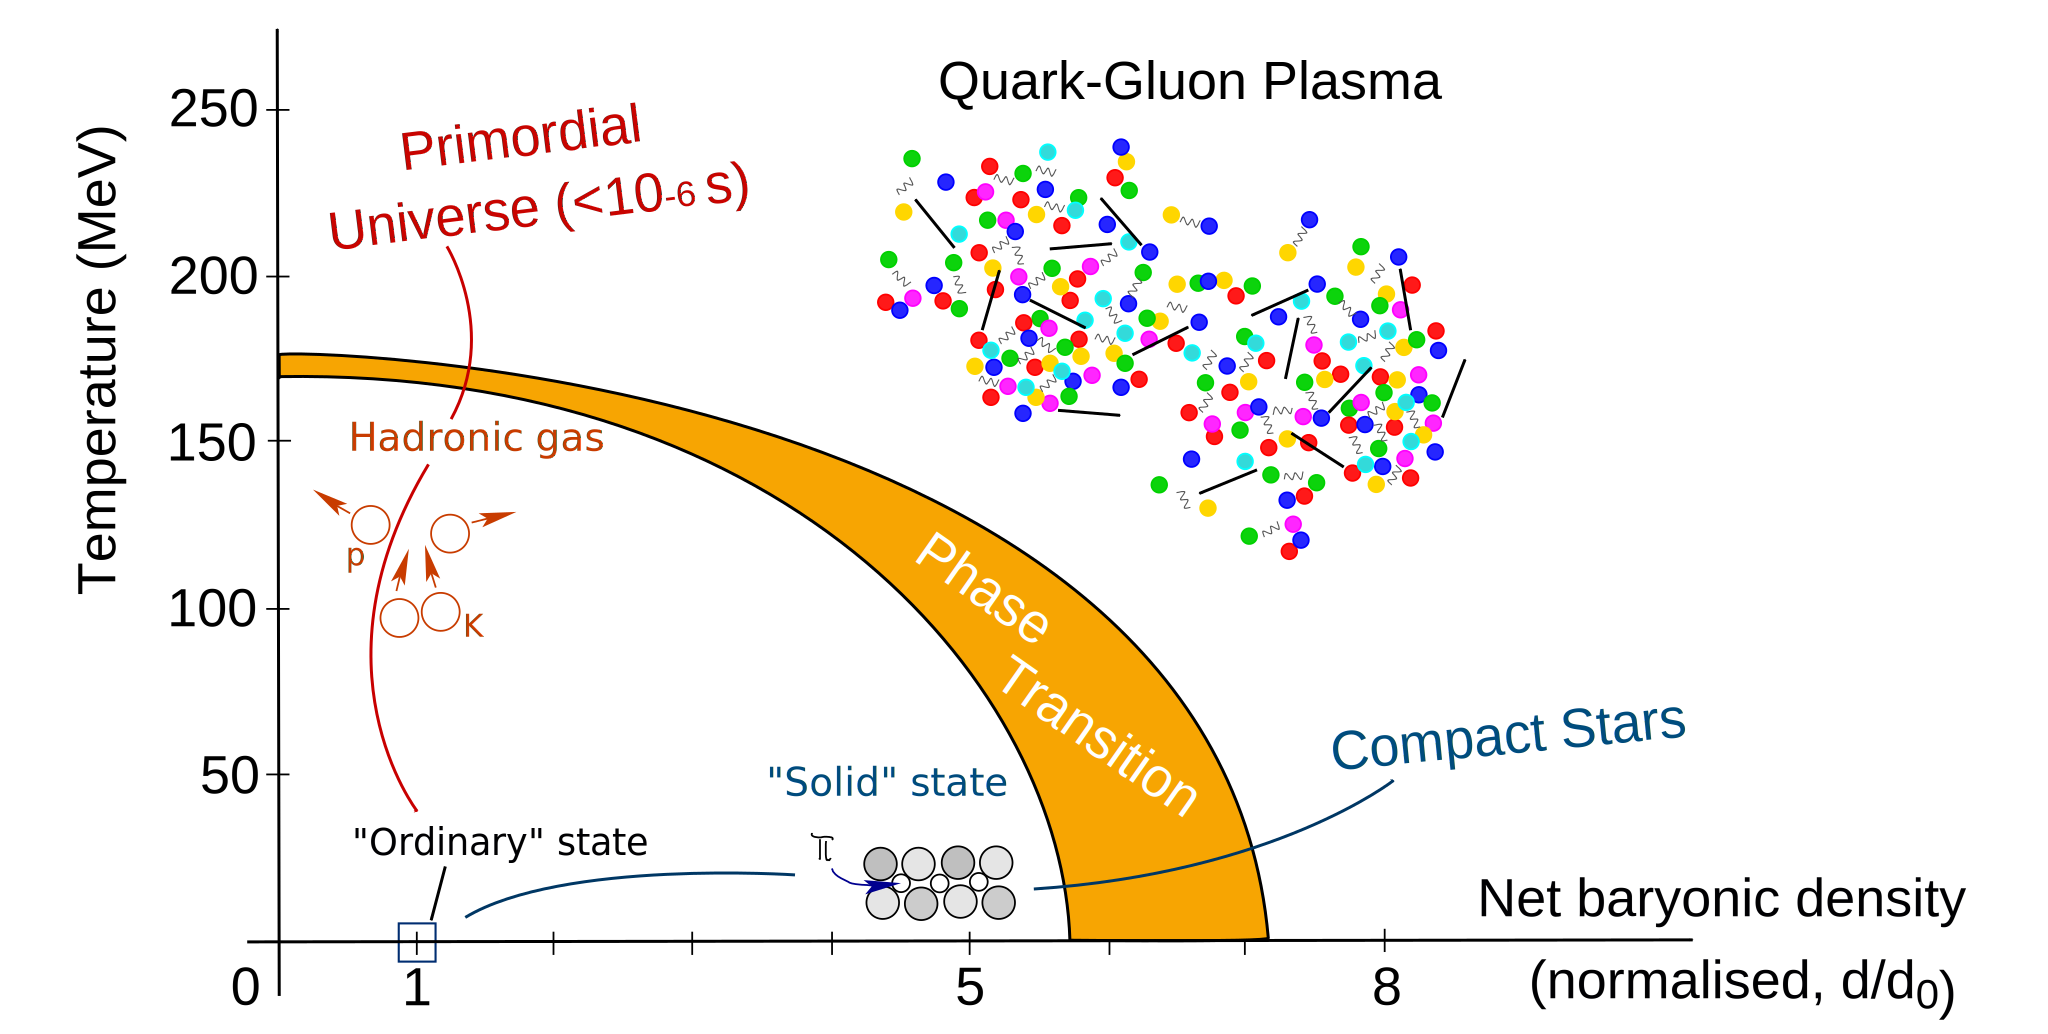
\includegraphics[width=0.9\textwidth]{figures/qcd-phase-diagram.pdf}
\caption{%
	Slice of the phase diagram of quantum chromodynamics with zero isospin and strangeness.
	\credit{CERN / Antonin Maire}{https://cds.cern.ch/record/2025215}
}
\label{fig:qcd:phase_diagram}
\end{figure}

The phase diagram of quantum chromodynamics describes the phase of quark matter as a function of temperature $T$, the quark chemical potential $\mu_Q$, the isospin chemical potential $\mu_I$ and the strangeness chemical potential $\mu_S$.
Although mapping out the diagram is an active area of research, a rough qualitative picture is known, and the slice with $\mu_I = \mu_S = 0$ is shown in \cref{fig:qcd:phase_diagram}.
Later we will see that the state of matter in compact stars is parametrized by a curve in the phase diagram that lies close to the $\mu_Q$-axis, corresponding to the density of baryons.
We will shortly discuss the most important qualitative properties of quantum chromodynamics and relate them to this phase diagram.

Quantum chromodynamics is notorious for being very difficult to make analytical calculations with, and its elegance and practicality stops not longer after writing down its Lagrangian \eqref{eq:qcd:lagrangian}.
To explore the phase diagram, one must therefore resort to alternative techniques:
\begin{itemize}
\item \textbf{Perturbation theory} can be used to study quantum chromodynamics at \emph{high} energy, perhaps contrary to what one might expect.
      As we will soon discuss in more detail, this is due to a property called asymptotic freedom that causes the interaction strength to \emph{decrease} with increasing energy.
\item \textbf{Lattice QCD} consists of making numerical calculations on a discrete lattice of spacetime points.
      This method has proved very useful for studying quantum chromodynamics under quite general circumstances.
      In the regime of high density and low temperature, however, is plagued by the so-called sign problem that refers to the difficulty of calculating integrals of highly oscillatory functions.
      This is precisely the area in the phase diagram that is relevant for compact stars.
\item The \textbf{$\bm{1/N_c}$-approximation} or \textbf{large $\bm{N_c}$-limit} consists of making expansions in the assumed small parameter $1/N_c$.
      Although there are only $N_c = 3$ colors in nature, this scheme has indeed been used to make accurate predictions.
      We will refer to this approximation to justify some of our later actions.
\item \textbf{Effective theories and models} can be used to study quantum chromodynamics in some regimes of interest.
      The most important requirements of such a theory or model is that it includes the correct degrees of freedom (or particles) and exhibit the same symmetries and symmetry breaking patterns as the theory it aims to describe in the regime of interest.
      Due to \cite{ref:weinberg_eft}, the philosophy is then to ``write down the most general possible theory involving fields for these particles, including all possible interactions consistent with the symmetries''.
      For example, chiral perturbation theory ($\chi$PT), the Nambu-Jona-Lasinio (NJL) model and the linear sigma model (LSM), also known as the quark-meson (QM) model, all give effective descriptions of quantum chromodynamics at low energies.
      This approach is applicable to compact stars and is the one we will take.
\end{itemize}

\subsubsection{Color confinement and asymptotic freedom \cite{ref:quark_bag_model}}

\begin{figure}
\centering
\tikzsetnextfilename{bag-model}
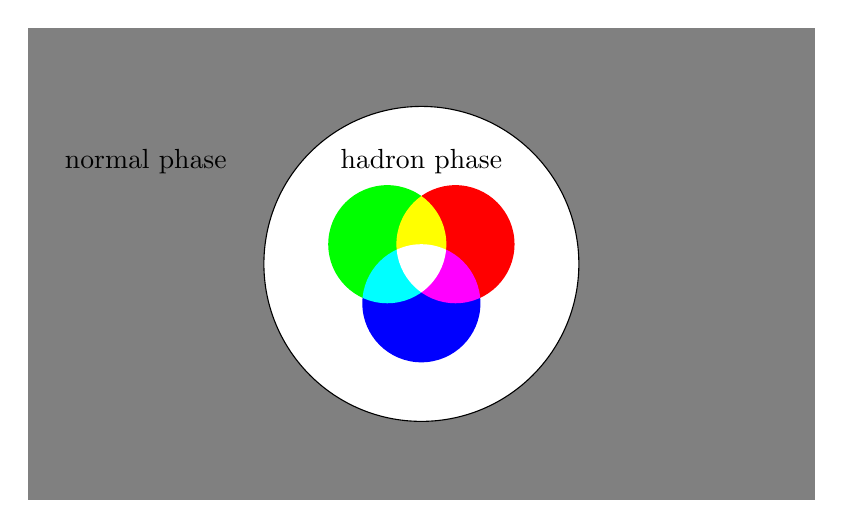
\begin{tikzpicture}
\fill [gray] (-5, -3) rectangle (+5, +3);

\draw [draw=black, fill=white] (0, 0) circle (2);
\begin{scope}[blend group=screen]
	\fill [fill=red]   (30:0.5)  circle (0.75) node {$u$};
	\fill [fill=green] (150:0.5) circle (0.75) node {$d$};
	\fill [fill=blue]  (270:0.5) circle (0.75) node {$s$};
\end{scope}
\node at (90:1.3) {hadron phase};
\node at (-3.5,1.3) {normal phase};
\end{tikzpicture}
\caption{\label{fig:lsm:confinement}%
	\TODO{caption}
}
\end{figure}

One fundamental feature of quantum chromodynamics is \textbf{color confinement}.
Quarks can be color-charged \textcolor{red}{\textbf{red}}, \textcolor{green}{\textbf{green}} and \textcolor{blue}{\textbf{blue}},
while antiquarks can have the complementary anticolors \textcolor{cyan}{\textbf{antired}}, \textcolor{magenta}{\textbf{antigreen}} and \textcolor{yellow}{\textbf{antiblue}}.
At low temperature and density, experiments and lattice simulations show that quarks never appear in isolation, but are always confined in hadrons that have no overall color.
As the distance between color-charged quarks increases, the strong force between them remains \emph{constant} -- the quarks are  effectively ``glued'' together by the mediating gluon.
For example, a meson consists of one quark of any color and one antiquark of its complementary color, making the meson itself colorless or ``white''.
Similarly, a(n) (anti)baryon consists of one (anti)red, one (anti)green and one (anti)blue quark and is also ``white''.

What if an even stronger force overcomes the strong force and tries to forcibly separate the quarks in a hadron into colorful groups of quarks?
Then nature will simply create new quark--anti-quark pairs so that the new groups of quarks both become new colorless hadrons.
\TODO{Figure} illustrates this process for a meson.
At low temperatures and densities in the lower left of \cref{fig:qcd:phase_diagram}, quarks are therefore \emph{confined} in colorless hadronic matter that make up the present world around us.

In the opposite extreme, quantum chromodynamics displays the property of \textbf{asymptotic freedom}.
As the energy scale of quark interactions increases, or equivalently its length scale decreases, the interaction strength \emph{decreases}.
When the density reaches extreme levels, confined hadronic quark matter then turns into a \emph{deconfined} \textbf{quark-gluon plasma} in the upper right of \cref{fig:qcd:phase_diagram} where they are free of all interactions and move around at will.
It is believed that the universe passed through this phase during the first $\SI{20}{\micro\second}$ after the Big Bang, after which it transitioned to the present phase of hadronic matter.
As no human-made laboratory can possibly recreate the necessary densities in the near future, the best candidates for finding and studying this exotic state of matter today is precisely the cores of compact stars.
Asymptotic freedom was first discovered by \cite{ref:asymptotic_freedom_gross_wilczek,ref:asymptotic_freedom_politzer}, who were recognized with the Nobel Prize in 2004.

\subsubsection{Vector, axial and chiral symmetries and chiral symmetry breaking}

The Lagrangian \eqref{eq:qcd:lagrangian} has some interesting global symmetries, each of which gives rise to a conserved classical current by Noether's theorem.
The simplest symmetry is the $U(1)_V$ \textbf{vector symmetry} $q \rightarrow e^{i \theta} q$, giving rise to the conserved vector current $j^\mu = \bar{q} \gamma^\mu q$ representing the baryon number density.
In the grand canonical ensemble, we will later couple one such conserved current to a chemical potential for each quark flavor.
In the massless case $m = 0$, the Lagrangian also has the $U(1)_A$ \textbf{axial symmetry} $q \rightarrow e^{i \theta \gamma^5} q$ with the conserved axial current $j^\mu = \bar{q} \gamma^\mu \gamma^5 q$.
As its proof assumes the action to be extremized, Noether's theorem is inherently \emph{classical}.
Unlike the vector current, the axial current is no longer conserved under the influence of quantum effects, and is therefore said to be \emph{anomalous}.

Using the projection operator $P_\pm = \frac12 (1 \pm \gamma^5)$, we can introduce the left-handed ($-$) and right-handed ($+$) chiral fields $q_\pm = P_\pm q$.
One can then show that $q = q_- + q_+$, $\bar{q}_\pm q_\pm = 0$ and $\bar{q}_\pm \gamma^\mu D_\mu q_\mp = 0$, so that the Lagrangian \eqref{eq:qcd:lagrangian} can be written
\begin{equation}
	\lagr = \bar{q}_- i \gamma^\mu D_\mu q_- + \bar{q}_+ i \gamma^\mu D_\mu q_+ - \bar{q}_- m q_+ - \bar{q}_+ m q_- - \frac14 G_{\mu\nu}^a G^{\mu\nu}_a.
\label{eq:qcd:lagrangian_chiral}
\end{equation}
In the massless case $m=0$,
it is left invariant under the $SU(N_f)_L \times SU(N_f)_R$ \textbf{chiral symmetry} transformation $q_\pm \rightarrow U_\pm q_\pm$ where both $U_\pm \in SU(N_f)$.
Moreover, it is known that the ground state of quantum chromodynamics admits a nonzero quark condensate \cite[chapter 28]{ref:schwartz}
\begin{equation}
	\avg{\bar{q} q} %= \avg{\bar{q}_- q_-} + \avg{\bar{q}_+ q_+} + \avg{\bar{q}_- q_+} + \avg{\bar{q}_+ q_-}
	                                                            = \avg{\bar{q}_- q_+} + \avg{\bar{q}_+ q_-},
\end{equation}
which is generally \emph{not} invariant under the chiral transformation.
The fact that the ground state does not carry the same symmetry as its Lagrangian is the signature of \textbf{spontaneous symmetry breaking}.
Only if $U_- = U_+$ are all terms invariant -- this is the $SU(N_f)_V$ \textbf{isospin symmetry} where both left-handed and right-handed fields are transformed in the same way.
The isospin symmetry is also a symmetry of the \emph{massive} Lagrangian \eqref{eq:qcd:lagrangian_chiral} \emph{if} all quark masses are set equal so that the mass matrix $m$ proportional to the identity matrix.
We therefore say that quantum chromodynamics exhibits \textbf{chiral symmetry breaking}
\begin{equation}
	SU(N_f)_L \times SU(N_f)_R \quad (m = 0) \qquad \rightarrow \quad SU(N_f)_V \quad (m \neq 0).
\end{equation}
Goldstone's theorem then predicts that one massless Goldstone boson arises from every broken symmetry generator.
Hence, chiral symmetry breaking gives rise to $2 \times (N_f^2 - 1) - (N_f^2 - 1) = N_f^2 - 1$ Goldstone bosons.
With $N_f = 2$ and $N_f = 3$ flavors, these are the three pions and the eight light pseudoscalar mesons.

In the real world, however, the quarks have different masses and cause the chiral symmetry to be only \emph{approximately} broken.
We say that the different quark masses cause \textbf{explicit symmetry breaking}, in the sense that the Lagrangian changes by a small amount under the chiral transformation.
The physical consequence of this is that there are no massless Goldstone bosons, but rather very light pseudo-Goldstone bosons.

The breaking of chiral symmetry leads to the \textbf{chiral phase transition} colored orange in \cref{fig:qcd:phase_diagram},
connecting the phases of hadronic quark matter and quark-gluon plasma.


\pagebreak
\TODO{move below to LSM discussion?}

Quark-meson model can be written in terms of left/right fields:
\begin{equation}
\begin{split}
	\bar{\psi} \phi_5 \psi &= \bar{\psi} ( (P_+ + P_-) \sigma + (P_+ - P_-) i \tau \cdot \pi) \psi \\
	                       &= \bar{\psi} ( P_+ (\sigma + i \tau \cdot \pi) + P_- (\sigma - i \tau \cdot \pi) ) \psi \\
	                       &= \bar{\psi} ( P_+ \phi + P_- \phi^\dagger) \psi \\
	                       &= \bar{\psi} ( P_+ \phi P_+ + P_- \phi^\dagger P_-) \psi \\
	                       &= \bar{\psi}_- \phi P_+ + \bar{\psi}_+ \phi^\dagger \psi_- \\
\end{split}
\end{equation}
Used that $P_\pm^2 = P_\pm$ is in spinor-space, while $\phi$ is in flavor space.
Denote $+ = R$, $- = L$.
Now it is apparent that LSM is invariant under $SU(2)_L \times SU(2)_R$:
\begin{equation}
	\psi_+ \rightarrow U_+ \psi_+, \qquad
	\psi_- \rightarrow U_- \psi_-, \qquad
	\phi   \rightarrow U_- \phi U_+^\dagger.
\end{equation}
When $h \neq 0$, this symmetry is explicitly broken.


\TODO{what about radius $r < R$ instead of $r=R$?}

\TODO{what about general relativity instead of Newtonian gravity?}

\TODO{what about contribution from pressure and other things to $F_\text{out}$?}

\TODO{can I recast inequality in charge per solar mass? see discussion at beginning of \url{www.if.ufrgs.br/hadrons/MMalheiro.pdf}}

\TODO{discuss $\epsilon$, $P$ before this}
\TODO{understand bag-constant as a measure of the trace anomaly? $m = 0$ -- conformal inveriance, classical symmetry broken in the quantum case?}
\TODO{justify and make less ad-hoc, move some of this to intro?}
\TODO{understand difference between $P(\mu)$ and $P(\mu,B)$}
\TODO{find source on bag stuff. JO?}
\TODO{difference between ``perturbative vacuum'' and ``confined vacuum''}

\chapter{Tolman-Oppenheimer-Volkoff equation}

TODO: write intro after I know everything we should do in this section

TODO: add page numbers to citations

\section{Derivation from the Einstein field equations}
\label{sec:tov}

To analyze astrophysical objects like stars, it is of considerable interest to relate the pressure $p(x)$ and energy density $\epsilon(x)$ or mass density $\rho(x)$ at every position $x$ inside the object.
We will derive the relativistic relation between these quantities from the \textbf{Einstein field equations} \cite[equation 4.44]{ref:carroll}
\begin{equation}
	G\indices{_\mu_\nu} = R_{\mu \nu} - \frac{1}{2} R g_{\mu \nu} = \frac{8 \pi G}{c^4} T_{\mu \nu} .
	\label{eq:einstein}
\end{equation}
It describes how the geometry of spacetime, described by the Ricci tensor $R\indices{_\mu_\nu}$ and Ricci scalar $R$ that are ultimately built from the metric $g\indices{_\mu_\nu}$ and encapsulated in the Einstein tensor $G\indices{_\mu_\nu}$ (see \cref{chap:gr_summary} for a summary), responds to the presence of energy-momentum in the energy-momentum tensor $T\indices{_\mu_\nu}$.
Here, $G$ is the gravitational constant and $c$ is the speed of light.
As we later compare our findings to those of Newtonian gravity, it will be useful to connect the energy density to the mass density by the \textbf{mass-energy equivalence relation}
\begin{equation}
	\epsilon(x) = \rho(x) c^2 .
	\label{eq:tov:mass_energy_equivalence}
\end{equation}

Unless rotating very fast, stars are well approximated by spheres.
For our purposes, we therefore use the coordinates
\begin{equation}
	x^\mu = (c t, r, \theta, \phi)
	\quad \text{with} \quad
	-\infty < t < \infty, \quad
	0 \leq r < \infty, \quad
	0 \leq \theta \leq \pi, \quad
	0 \leq \phi < 2 \pi .
\end{equation}
and consider the most general line element that exhibits spherical symmetry, \cite[§ 94-95]{ref:tolman}
(TODO: do more general with $\gamma(r)$, as done in Carroll?)
\begin{equation}
	% coordinates x = (ct, r, θ, ϕ)
	\dif s^2 = -e^{2 \alpha(r)} c^2 \dif t^2 + e^{2 \beta(r)} \dif r^2 + r^2 \left( \dif \theta^2 + \sin^2 \theta \dif \phi^2 \right) .
\end{equation}

We model the interior of the star as a perfect fluid with energy-momentum \cite[equation 1.114]{ref:carroll}
\begin{equation}
	T\indices{_\mu_\nu} = \frac{1}{c^2} (\epsilon+p) U_\mu U_\nu + p g\indices{_\mu_\nu}.
\end{equation}
For a static star whose fluid is at rest, $U_\mu = (U_0, \textbf{0})$ and the normalization condition $U_\mu U^\mu = -c^2$ requires $U_0 = \pm e^\alpha c$.
We choose the positive sign so the four-velocity lies in the future light cone, as we are interested in the evolution of the star.
Then the energy-momentum tensor takes the diagonal form
\begin{equation}
T\indices{_\mu_\nu} =
\begin{bmatrix}
	\epsilon e^{2\alpha} & 0            & 0     & 0                   \\
	0                    & p e^{2\beta} & 0     & 0                   \\
	0                    & 0            & p r^2 & 0                   \\
	0                    & 0            & 0     & p r^2 \sin^2 \theta \\
\end{bmatrix}
\qquad \text{or} \qquad
T\indices{_\mu^\nu} =
\begin{bmatrix}
	-\epsilon & 0 & 0 & 0 \\
	0         & p & 0 & 0 \\
	0         & 0 & p & 0 \\
	0         & 0 & 0 & p \\
\end{bmatrix}
.
\label{eq:einstein_to_tov:T}
\end{equation}

Starting with the metric, it is now straightforward, although tedious, to compute the left side of \cref{eq:einstein} from \cref{eq:def_christoffel,eq:def_riemann_tensor,eq:def_ricci_tensor,eq:def_ricci_scalar}.
For the details, refer to \cite[equation 5.11-5.15]{ref:carroll}.
After inserting the energy-momentum tensor on the right and simplifying, we get the three independent equations
(the fourth turns out proportional to the third)
\begin{subequations}
\begin{align}
	\frac{1}{r^2} e^{-2 \beta} \left( 2 r \beta' - 1 + e^{2 \beta} \right)                               &= \frac{8 \pi G}{c^4} \epsilon
	&& \left( G\indices{_0_0} = \frac{8 \pi G}{c^4} T\indices{_0_0} \right) , \label{eq:einstein_to_tov:tt} \\
	\frac{1}{r^2} e^{-2 \beta} \left( 2 r \alpha' + 1 - e^{2 \beta} \right)                              &= \frac{8 \pi G}{c^4} p
	&& \left( G\indices{_1_1} = \frac{8 \pi G}{c^4} T\indices{_1_1} \right) , \label{eq:einstein_to_tov:rr} \\
	e^{-2 \beta} \left( \alpha'' + (\alpha')^2 - \alpha' \beta' + \frac{1}{r} (\alpha' - \beta') \right) &= \frac{8 \pi G}{c^4} p
	&& \left( G\indices{_2_2} = \frac{8 \pi G}{c^4} T\indices{_2_2} \right) . \label{eq:einstein_to_tov:thetatheta}
\end{align}
\end{subequations}

Next, let us introduce the mass of the star.
Define the function $m(r)$ by
\begin{equation}
	e^{2 \beta} = \left( 1 - \frac{2 G m(r)}{r c^2} \right)^{-1} ,
	\label{eq:einstein_to_tov:def_m}
\end{equation}
so $g\indices{_1_1}$ resembles the Schwarzschild metric element.
Then \cref{eq:einstein_to_tov:tt} becomes
\begin{equation}
	\diff{(m c^2)}{r} = 4 \pi r^2 \epsilon(r) ,
	\label{eq:einstein_to_tov:m_rho}
\end{equation}
directly relating $m(r)$ and $\epsilon(r)$.
If we set $m(0) = 0$, we can integrate to get
\begin{equation}
	m(r) c^2 = \integral{\epsilon(r') 4 \pi r'^2}{r'}{0}{r} .
	\label{eq:einstein_to_tov:m_integral}
\end{equation}
\cite[page 602]{ref:mtw} shows that setting $m(0) \neq 0$ creates a singularity at the origin, which is not physically acceptable.
Outside a star that extends to $r = R$, there is vacuum with $\epsilon = 0$ and our metric should match the Schwarzschild metric with $g\indices{_1_1} = (1-2GM/rc^2)^{-1}$ and Schwarzschild mass $M$.
By comparison with \cref{eq:einstein_to_tov:def_m}, the \textbf{Schwarzschild mass} of the star must be
\begin{equation}
	M = m(R) = \frac{1}{c^2} \integral{\epsilon(r) 4 \pi r^2}{r}{0}{R} = \integral{\rho(r) 4 \pi r^2}{r}{0}{R}.
	\label{eq:einstein_to_tov:schwarzschild_mass}
\end{equation}
It is tempting to interpret the Schwarzschild mass $M$ as the Newtonian mass of the star and \eqref{eq:einstein_to_tov:m_integral} as the volume integral of the energy density $\epsilon(r)$.
But $4 \pi r^2$ is not a proper volume element, as it does not involve the full spatial metric determinant.
We return to this question in \cref{sec:weak_field_limit} after studying incompressible stars in \cref{sec:incompressible_star}, where we will see that the first interpretation is correct, while the latter is more subtle and differs by the binding energy of the star.

Meanwhile, definition \eqref{eq:einstein_to_tov:def_m} turns \cref{eq:einstein_to_tov:rr} into
\begin{equation}
	\diff{\alpha}{r} = \frac{G}{r^2 c^4} \frac{m(r) c^2 + 4 \pi r^3 p}{1 - 2 G m(r) / r c^2} .
	\label{eq:einstein_to_tov:dadr1}
\end{equation}
To finally eliminate $\alpha$, we can replace all occurences of $\alpha'$ and $\beta$ in the remaining \cref{eq:einstein_to_tov:thetatheta} with the expressions \eqref{eq:einstein_to_tov:dadr1} and \eqref{eq:einstein_to_tov:def_m}.
Doing so is straightforward, but cumbersome and most easily done by a computer algebra system.
We show how to do this in \cref{sec:tov_cas_derivation}.
An elegant, but less straightforward argument is to use local energy-momentum conservation $\nabla_\mu T\indices{^\mu^\nu} = 0$, which is both physically reasonable and in fact possible to prove directly from the Einstein field equations \eqref{eq:einstein}.
For two different proofs, see \cite{ref:einstein_conservation_energy_momentum} and \cite[section 8.3.2]{ref:mika_gr_notes}.
Using \cref{eq:def_cov_deriv}, the $\nu=1$-component gives
\begin{equation*}
	0
	= \nabla_\mu T\indices{^\mu_1}
	= \partial_1 T\indices{^1_1} + \Gamma^\sigma_{1 \sigma} T\indices{^1_1} - \Gamma^\sigma_{1 \mu} T\indices{^\mu_\sigma}
	= \partial_1 T\indices{^1_1} + \Gamma^0_{10} T\indices{^1_1} + \sum_{i=1}^3 \Gamma^i_{1i} T\indices{^1_1} - \Gamma^0_{10} T\indices{^0_0} - \sum_{i=1}^3 \Gamma^i_{1i} T\indices{^i_i}
\end{equation*}
Using $T\indices{^0_0} = -\epsilon$ and $T\indices{^1_1} = T\indices{^2_2} = T\indices{^3_3} = p$ from \cref{eq:einstein_to_tov:T}, the sums cancel, leaving
\begin{equation}
	\diff{\alpha}{r} = \frac{-1}{\epsilon+p} \diff{p}{r} .
	\label{eq:einstein_to_tov:dadr2}
\end{equation}
Now $\alpha$ is easily eliminated by equating \eqref{eq:einstein_to_tov:dadr1} and \eqref{eq:einstein_to_tov:dadr2}. 
Whichever approach we follow, we end up with the \textbf{Tolman-Oppenheimer-Volkow (TOV) equation}
\begin{equation}
	\diff{p}{r} = -\frac{G m(r) \epsilon(r)}{r^2 c^2} \left( 1 + \frac{p(r)}{\epsilon(r)} \right) \left( 1 + \frac{4 \pi r^3 p(r)}{m(r) c^2} \right) \left( 1 - \frac{2 G m(r)}{r c^2} \right)^{-1} .
	\label{eq:tov}
\end{equation}
It relates the pressure gradient $\diff{p}{r}$ and energy density $\epsilon$ at radius $r$ from the center of a spherical static star composed of a perfect fluid.
\Cref{eq:einstein_to_tov:m_rho,eq:tov} constitute two equations for the three unknowns $p$, $\epsilon$ and $m$.
To determine them, an additional \textbf{equation of state}
\begin{equation}
	F(p, \epsilon) = 0
\end{equation}
that relates the thermodynamic variables is required, typically obtained from statistical physics.
Given all three equations and the central pressure $p(0)$, we can integrate to find the pressure everywhere inside the star.
We define the radius of the star to be the radius $R$ at which $p(R) = 0$.
Carrying out this procedure for different values of $p(0)$, we can find a mass-radius relation $M(R)$ for stars parametrized by their central pressure $p(0)$.

The TOV equation was originally derived by \cite{ref:tov} using multiple results from \cite{ref:tolman}.

\section{Solution for an incompressible star}
\label{sec:incompressible_star}

% TODO: an incompressible star is unphysical

Although it may sound unphysical from the outset, we can make a somewhat realistic model of a star by assuming that the fluid is incompressible, meaning the energy density
\begin{equation}
	\epsilon(r) = \epsilon_0
\end{equation}
is constant inside the star.
For example, this results in a completely unrealistic speed of sound $v = \sqrt{\difft{p}{\rho}} = c \sqrt{1/(\difft{\epsilon}{p})} = c \sqrt{1/0} = \infty$. \cite{ref:speed_of_sound}
Anyway, integrating \cref{eq:einstein_to_tov:m_integral,eq:einstein_to_tov:schwarzschild_mass} yield
\begin{equation}
	m(r) c^2 = \frac{4}{3} \pi r^3 \epsilon_0 
	\quad \text{and} \quad
	M c^2 = \frac{4}{3} \pi R^3 \epsilon_0 
	.
\end{equation}
Inserting the energy density $\epsilon(r)$ and mass $m(r)$ into \cref{eq:tov}, $p$ and $r$ separate to
\begin{equation*}
	\int \frac{\dif p}{(\epsilon_0+p)(\epsilon_0+3p)} = - \int \frac{4 \pi G r \dif r}{3 c^4 - 8\pi G r^2 \epsilon_0} .
\end{equation*}
The left side can now be split by the partial fraction decomposition
\begin{equation*}
	\frac{1}{(\epsilon_0+p)(\epsilon_0+3p)} = \frac{1}{2p} \left( \frac{1}{\epsilon_0+p} + \frac{1}{\epsilon_0+3p} \right) .
\end{equation*}
Performing all three integrals using the general antiderivatives
\begin{equation*}
	\int \frac{\dif x}{a x^2 + b x} = -\frac{1}{b} \log \left( a + \frac{b}{x} \right) + C
	\quad \text{and} \quad
	\int \frac{x \dif x}{a x^2 + b} = \frac{1}{2 a} \log \left( a x^2 + b \right) + C
\end{equation*}
and applying the boundary condition $p(R) = 0$ to determine the integration constant, we eventually find the radial pressure
\begin{equation}
	% p(r) in terms of M, R, 
	p(r) = \epsilon_0 \, \frac{\sqrt{1-\frac{2GMr^2}{R^3c^2}} - \sqrt{1-\frac{2GM}{Rc^2}}}{3 \sqrt{1-\frac{2GM}{Rc^2}} - \sqrt{1-\frac{2GMr^2}{R^3c^2}}} .
	% p(r) in terms of p0, M, R
	%p(r) = -\frac{M}{\frac{4}{3} \pi R^3} \frac{4 \pi R^{3} p_0 \left( \frac{1}{3} + \sqrt{1-\frac{2GMr^2}{R^3}} \right) + M \left( 1 + \sqrt{1-\frac{2GMr^2}{R^3}} \right)}
	%                                           {4 \pi R^{3} p_0 \left( 1           + \sqrt{1-\frac{2GMr^2}{R^3}} \right) + M \left( 3 + \sqrt{1-\frac{2GMr^2}{R^3}} \right)}
	\label{eq:incompressible_star:pressure}
\end{equation}
In particular, the central pressure is
\begin{equation}
	p(0) = \epsilon_0 \frac{1 - \sqrt{1 - \frac{2GM}{Rc^2}}}{3 \sqrt{1-\frac{2GM}{Rc^2}} - 1} .
	\label{eq:incompressible_star:central_pressure}
\end{equation}
It is interesting to note that the pressure is positive for $GM/Rc^2 < 4/9$, but explodes at $GM/Rc^2 = 4/9$ and becomes negative for $GM/Rc^2 > 4/9$.
Physically, this means that once a star with fixed radius becomes massive enough, it implodes and turns into a black hole.
This is an example of a more general result -- \textbf{Buchdal's theorem} states that all static spherical stars composed of perfect fluids must have
\begin{equation}
	M(R) < M_\text{max}(R) = \frac{4c^2}{9G} R
	\label{eq:incompressible_star:buchdal}
\end{equation}
for any energy density distribution $\epsilon(r)$ that does not decrease outwards. \cite{ref:buchdal}
The proof requires careful work, but we can still understand the result intuitively.
An object with a mass-energy distribution that somehow satures the limit set by nature itself should have the same density everywhere.
If it does not, there will be a place with lower density than its surroundings, which in turn will generate a pressure gradient force that seeks to establish equilibrium by eliminating the difference in density.
Thus, the bound we have found in our computation with constant energy density should be the most extreme bound.

In \cref{sec:weak_field_limit} we will see that Buchdal's theorem is a relativistic result and that no such bound arises from Newtonian gravity.

\begin{figure}[hb!]
\centering

% TODO: cannot use JO length scale (it evolves ϵ, and i have different ϵ)
% TODO: use sun mass and radius ?
% how to center subcaptions under/over xlabel/plot area: 
%   trim axis left/right: https://tex.stackexchange.com/a/134262
% + hfil: https://tex.stackexchange.com/a/321476
%   (not working properly)
% ideal use of groupplot + subcaption: https://tex.stackexchange.com/a/310403
\begin{subfigure}{0.49\textwidth}
	\caption{\label{fig:incompressible_star:plot1}Mass-radius relation}
	\begin{tikzpicture}
	\begin{axis}[
		width=1.00\textwidth, 
		xlabel=$R \, / \, R_0$, ylabel=$M(R) \, / \, M(R_0)$, xtick distance=1, 
		legend pos=north west, legend cell align=left, declare function={
			G = 1;
			M(\R,\E) = 4/3*pi*(\R)^3*\E;
			Mmax(\R) = 4*\R/(9*G);
		}
	]
		\pgfplotsinvokeforeach{0.006} {
			\addplot [domain=0:5, solid ] {M(x,#1) / M(1,#1)}; % node[pos=0.90, sloped, yshift=+6pt] {\scriptsize $\epsilon_0 = #1$};
			\addplot [domain=0:5, dashed] {Mmax(x) / M(1,#1)}; % node[pos=0.2, pin=above:{$M_\text{max}(R)$}] {};
		}
		\legend{$M(R)$, $M_\text{max}(R)$};
	\end{axis}
	\end{tikzpicture}
\end{subfigure}
\hfill
\begin{subfigure}{0.49\textwidth}
	\caption{\label{fig:incompressible_star:plot2}Pressure distribution}
	\begin{tikzpicture}
	\begin{axis}[
		width=1.00\textwidth,
		xlabel=$r\, /\, R_0$, ylabel=$p(r) \, / \, p(0)$, xtick distance=0.25, declare function={
			G=1;
			R=2;
			p(\r,\M) = \M / (4/3*pi*R^3) * (sqrt(1-2*G*\M*(\r)^2/R^3) - sqrt(1-2*G*\M/R)) / (3*sqrt(1-2*G*\M/R) - sqrt(1-2*G*\M*(\r)^2/R^3));
			Mmax = 4*R/(9*G);
		}
	]
	\pgfplotsinvokeforeach{0.9, 0.99, 0.999} {
		\addplot [domain=0:1,samples=200] {p(x*R,#1*Mmax)/p(0,#1*Mmax)} node[pos=0.54, sloped, yshift=+16pt] {\scriptsize $M = #1 M_\text{max}$};
	}
	\end{axis}
	\end{tikzpicture}
\end{subfigure}
\caption{
	\subref{fig:incompressible_star:plot1} Mass-radius relation $M(R) = 4 \pi R^3 \epsilon_0 / 3 c^2$ for a star of constant energy density $\epsilon_0$ compared to the maximum supported mass $M_\text{max}(R) = 4 c^2 R / 9 G$.
	\subref{fig:incompressible_star:plot2} Pressure distribution $p(r)$ for stars of the same radius $R_0$, but different energy densities $\epsilon_0$ and masses $M$ approaching $M_\text{max}(R)$.
	Here, $R_0 = \sqrt{c^4 / G \epsilon_0}$ is a length scale. % and $M_0 = 4 \pi R_0^3 \epsilon_0 / 3$ is a mass scale.
}
\iffalse
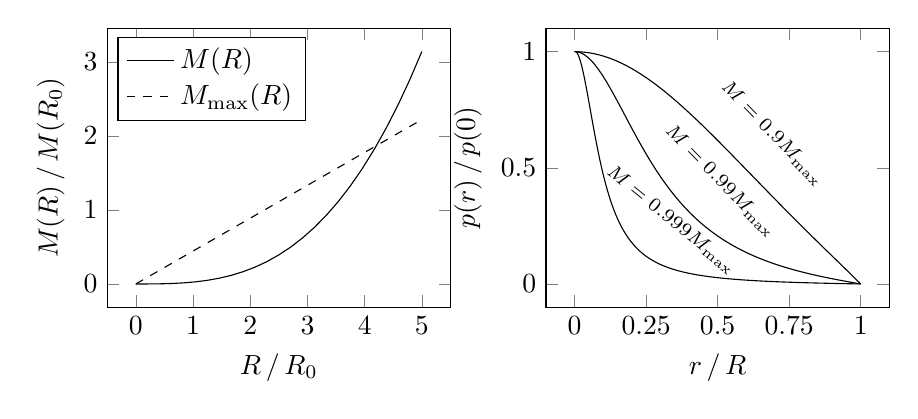
\begin{tikzpicture}
\begin{groupplot}[group style={group size=2 by 1, horizontal sep=0.1\textwidth}, width=0.49\textwidth]
	% TODO: cannot use JO length scale (it evolves ϵ, and i have different ϵ)
	% TODO: use sun mass and radius ?
	\nextgroupplot[xlabel=$R \, / \, R_0$, ylabel=$M(R) \, / \, M(R_0)$, xtick distance=1, legend pos=north west, legend cell align=left, declare function={
		G = 1;
		M(\R,\E) = 4/3*pi*(\R)^3*\E;
		Mmax(\R) = 4*\R/(9*G);
	}]
	\pgfplotsinvokeforeach{0.006} {
		\addplot [domain=0:5, solid ] {M(x,#1)}; % node[pos=0.90, sloped, yshift=+6pt] {\scriptsize $\epsilon_0 = #1$};
	}
	\addplot [domain=0:5, dashed] {Mmax(x)}; % node[pos=0.2, pin=above:{$M_\text{max}(R)$}] {};
	\legend{$M(R)$, $M_\text{max}(R)$};
	\nextgroupplot[xlabel=$r\, /\, R$, ylabel=$p(r) \, / \, p(0)$, xtick distance=0.25, declare function={
		G=1;
		R=2;
		p(\r,\M) = \M / (4/3*pi*R^3) * (sqrt(1-2*G*\M*(\r)^2/R^3) - sqrt(1-2*G*\M/R)) / (3*sqrt(1-2*G*\M/R) - sqrt(1-2*G*\M*(\r)^2/R^3));
		Mmax = 4*R/(9*G);
	}]
	\pgfplotsinvokeforeach{0.9, 0.99, 0.999} {
		\addplot [domain=0:1,samples=200] {p(x*R,#1*Mmax)/p(0,#1*Mmax)} node[pos=0.54, sloped, yshift=+16pt] {\scriptsize $M = #1 M_\text{max}$};
	}
\end{groupplot}
\end{tikzpicture}
\caption{
	Mass-radius relation $M(R) = 4 \pi R^3 \epsilon_0 / 3 c^2$ for a star of constant energy density $\epsilon_0$ compared to the maximum supported mass $M_\text{max}(R) = 4 c^2 R / 9 G$. Pressure distribution $p(r)$ for particular stars with radius $R=2$ and different masses $M$ approaching $M_\text{max}(R)$.}
	Here, $R_0 = \sqrt{c^4 / G \epsilon_0}$ is a length scale. % and $M_0 = 4 \pi R_0^3 \epsilon_0 / 3$ is a mass scale.
\fi
\end{figure}

\section{Weak-field limit and physical interpretation of mass}
\label{sec:weak_field_limit}

%TODO: move everything about interpretation of mass, energy density integral etc. to one section which has one thing in common: we look at the weak-field limit
%TODO: do weak-field limit of TOV equation, too

As we mentioned in \cref{sec:tov}, it is not apparent how to interpret the ``mass'' $M$ or ``energy'' $Mc^2$ in \cref{eq:einstein_to_tov:schwarzschild_mass}.
Here we will compare the results we have found so far to those of Newtonian gravity in the limit where particles move \emph{slowly} and the gravitational field is \emph{static} and \emph{weak}.

In Newtonian gravity, a particle is accelerated by the gravitational field
\begin{equation}
	\mathbf{g}(x) = - \nabla V(x) ,
	\label{eq:interpretation_m:newton2}
\end{equation}
where the gravitational potential $V$ is the solution to the Poisson equation
\begin{equation}
	\nabla^2 V(x) = 4 \pi G \rho(x) .
	\label{eq:interpretation_m:poisson}
\end{equation}

In general relativity, freely falling particles move along geodesics $x(\tau)$ that satisfy the \textbf{geodesic equation}
\begin{equation}
	\diff[2]{x^\mu}{\tau} + \Gamma^\mu_{\rho \sigma} \diff{x^\rho}{\tau} \diff{x^\sigma}{\tau} = 0 .
	\label{eq:geodesic}
\end{equation}
A \emph{slowly} moving particle has velocity $\diff{x^\mu}{\tau}$ with spatial component $\diff{x^i}{t} \ll c$ and is thus dominated by the spatial component $\diff{t}{\tau} \approx 1$.
Then $\diff{x^i}{\tau} \ll \diff{x^0}{\tau}$ and the geodesic equation can be approximated by
\begin{equation*}
	\diff[2]{x^\mu}{\tau} + \Gamma^\mu_{00} \, c^2 \left( \diff{t}{\tau} \right)^2 = 0 .
\end{equation*}
A \emph{static} field has $\partial_0 g\indices{_\mu_\nu} = 0$, so the Christoffel symbols \eqref{eq:def_christoffel} simplify to
\begin{equation*}
	\Gamma^\mu_{00} = \frac{1}{2} g\indices{^\mu^\lambda} (\partial_0 g\indices{_\lambda_0} + \partial_0 g\indices{_0_\lambda} - \partial_\lambda g\indices{_0_0}) = -\frac{1}{2} g\indices{^\mu^\lambda} \partial_\lambda g\indices{_0_0} .
\end{equation*}
A \emph{weak} gravitational field can be written as a perturbation 
\begin{equation}
	g\indices{_\mu_\nu} = \eta\indices{_\mu_\nu} + h\indices{_\mu_\nu}
	\quad \text{with} \quad
	\abs{h\indices{^\mu^\nu}} \ll 1
	\label{eq:weak_field_limit:metric_perturbation}
\end{equation}
on top of flat Minkowski space $\eta\indices{^\mu^\nu} = \text{diag}(-1, +1, +1, +1)$.
The inverse metric $g\indices{^\mu^\nu}$ should satisfy $g\indices{^\mu^\nu} g\indices{_\nu_\sigma} = \delta^\mu_\sigma$, so to first order in $h$ we must have
\begin{equation*}
	g\indices{^\mu^\nu} = \eta\indices{^\mu^\nu} - h\indices{^\mu^\nu} ,
\end{equation*}
where $h\indices{^\mu^\nu} = \eta\indices{^\mu^\rho} \eta\indices{^\nu^\sigma} h\indices{_\rho_\sigma}$ is raised with the Minkowski metric.
Calculating the relevant Christoffel symbols to first order in $h$, we find $\Gamma^\mu_{00} = -\frac{1}{2} \eta\indices{^\mu^\lambda} \partial_\lambda h\indices{_0_0}$, so the geodesic equation becomes
\begin{equation*}
	\diff[2]{x^\mu}{\tau} = \frac{1}{2} c^2 \eta\indices{^\mu^\lambda} \partial_\lambda h\indices{_0_0} \left( \diff{t}{\tau} \right)^2
	\quad \text{with spatial components} \quad
	\diff[2]{x^i}{t} = \frac{1}{2} c^2 \partial_i h\indices{_0_0} .
\end{equation*}
This is precisely \cref{eq:interpretation_m:newton2} if we identify $h\indices{_0_0} = -2V/c^2$ or $g\indices{_0_0} = -(1+2V/c^2)$, so a weak relativistic gravitational field $g\indices{_\mu_\nu} = \eta\indices{_\mu_\nu} + h\indices{_\mu_\nu}$ in fact describes Newtonian motion in the gravitational potential $V = -c^2 h\indices{_0_0} / 2$!
Moreover, the Schwarzschild metric has the element
\begin{equation}
	g\indices{_0_0} = - \left( 1 - \frac{2 G M}{r c^2} \right)
	\quad \text{with} \quad
	h\indices{_0_0} = 2GM/rc^2 ,
	\label{eq:weak_field_limit:schwarzschild_metric_tt}
\end{equation}
and $V = -c^2 h\indices{_0_0} / 2 = -G M / r$ is precisely the solution to Poisson's equation \eqref{eq:interpretation_m:poisson} for a spherical mass distribution, so general relativity does indeed describe Newtonian gravity in the weak-field limit!
In conclusion, this shows that it does make sense to interpret the Schwarzschild mass $M$ as the Newtonian mass of a star, as masses of distant stars are typically measured with results like Kepler's third law that follow from Newtonian gravity. \cite[box 23.1]{ref:mtw}

From the looks of \cref{eq:einstein_to_tov:schwarzschild_mass}, it is very tempting to also interpret $M c^2$ as the volume integral of the energy density over the star.
But $4 \pi r^2 \dif r$ is not a proper volume element.
In a proper spatial integral, the volume element should be $\sqrt{\abs{\gamma}} \dif^3 x = e^\beta r^2 \sin \theta \dif r \dif \theta \dif \phi$, where $\gamma\indices{_i_j} = g\indices{_i_j}$ is the spatial part of the metric and $\abs{\gamma}$ its determinant.
So the true volume integral of the energy density is really
\begin{equation*}
	\bar{M} c^2 = \integral{\epsilon(r) e^{\beta(r)} 4 \pi r^2}{r}{0}{R}.
\end{equation*}
The difference
\begin{equation*}
	\bar{M} c^2 - M c^2 = \integral{\epsilon(r) \left( \left( 1-\frac{2Gm}{rc^2} \right)^{-1/2} - 1 \right) 4 \pi r^2}{r}{0}{R} > 0
\end{equation*}
is in fact the binding energy that arises due to the gravitational attraction between the individual fluid elements in the star.
To see this, consider again the weak-field limit.
Comparing \cref{eq:weak_field_limit:metric_perturbation,eq:weak_field_limit:schwarzschild_metric_tt}, we see that we have the small parameter
\begin{equation}
	\frac{G m(r)}{rc^2} \ll 1 .
	\label{eq:weak_field_limit:small_gmr}
\end{equation}
Using the Taylor expansion $(1 - x)^{-1/2} = 1 + x/2$ and the mass-energy equivalence relation \eqref{eq:tov:mass_energy_equivalence}, we get
\begin{equation}
	\bar{M} c^2 - M c^2 \approx \integral{\frac{\epsilon(r)}{c^2} \frac{GM}{r} 4 \pi r^2}{r}{0}{R}
	                    =       \integral{\rho(r) \frac{GM}{r} 4 \pi r^2}{r}{0}{R} .
\end{equation}
As shown in \cite[exercise 23.7]{ref:mtw}, this is precisely the energy required to construct the star by sequentially placing thin shells of mass $\dif m = \rho(r) 4 \pi r^2 \dif r$ on top of each other, each subject to the gravitational attraction of the shells already placed below it.
This explains that $\bar{M} c^2 - M c^2$ is indeed the binding energy that would be required to disperse all the matter in the star to infinity.
% confusion about M, \bar{M}, resources:
% https://physics.stackexchange.com/q/196280/299916
% see MTW p. 602-, box at p. 603, p. 453
% see Schwarz p. 126

Finally, let us compare the TOV equation \eqref{eq:tov} and findings for relativistic incompressible stars from \cref{sec:incompressible_star} to those of Newtonian gravity.
To do so, we should first establish the Newtonian pressure gradient analogous to the relativistic one.

(TODO: figure for the below stuff)

Consider the mass element $\dif m = \rho(r) \dif A \dif r$ at distance $r$ from the center of a Newtonian star.
By Gauss' law it is attracted to the mass $m(r)$ inside the radius $r$ as if it were concentrated at the center, but experiences no attraction whatsoever from the remaining mass outside $r$ due to symmetry.
By Newton's law of gravity it is therefore pulled upon by the force
\begin{equation}
	\dif \mathbf{F}_1 = -\frac{G m(r) \dif m}{r^2} \hat{\textbf{r}} .
	\label{eq:weak_field_limit:force_newton}
\end{equation}
If the star is in hydrostatic equilibrium, this force must be exactly cancelled by the force
\begin{equation}
	\dif \textbf{F}_2 = - \Big( p(r + \dif r) - p(r) \Big) \dif A \, \hat{\textbf{r}} = -\dif p \dif A \, \hat{\textbf{r}}
	\label{eq:weak_field_limit:force_pressure}
\end{equation}
that arises from the pressure difference above and below the element.
Setting $\dif \textbf{F}_1 + \dif \textbf{F}_2 = 0$ then gives the \textbf{Newtonian pressure gradient}
\begin{equation}
	\diff{p}{r} = -\frac{G m(r) \rho(r)}{r^2} .
	\label{eq:weak_field_limit:newtonian_pressure_gradient}
\end{equation}

Solving this differential equation for a star of constant mass density $\rho(r) = \rho_0$ like we solved the TOV equation \eqref{eq:tov} in \cref{sec:incompressible_star}, we get the pressures
\begin{equation}
	p(r) = \frac{\rho_0}{2} \frac{G M}{R} \left( 1 + \frac{r}{R} \right) \left( 1 - \frac{r}{R} \right)
	\quad \text{and} \quad
	p(0) = \frac{\rho_0}{2} \frac{GM}{R} .
	\label{eq:weak_field_limit:newtonian_pressure}
\end{equation}
In this case, the pressure is well-behaved for all $r$.
This shows that Buchdal's theorem \eqref{eq:incompressible_star:buchdal} is a purely \emph{relativistic} result, and that no such limitation arises in Newtonian gravity!

% TODO: makes us suspect that Newton is taylor expansion of TOV
% TODO: check limit

Furthermore, we suspect that the relativistic pressure gradient \eqref{eq:tov} reduces to the Newtonian pressure gradient \eqref{eq:weak_field_limit:newtonian_pressure_gradient} in the Newtonian limit.
Comparing the two, we see that the relativistic equation indeed reduces to the Newtonian one if all the corrections to $1$ in the three parentheses vanish.
Let us see that this is actually the case.

First, note that by \cref{eq:weak_field_limit:small_gmr}, we have the small quantities
\begin{equation}
	\frac{Gm(r)}{rc^2} \ll 1
	\quad \text{and} \quad
	\frac{GM}{Rc^2} \ll 1 ,
	\label{eq:weak_field_limit:small3}
\end{equation}
so the rightmost correction in \cref{eq:tov} vanishes.

%By Taylor expanding the pressures \eqref{eq:incompressible_star:central_pressure} around the small parameter $GM/R \ll 1$, we get precisely the pressures in \cref{eq:weak_field_limit:newtonian_pressure}.
Second, we argued in \cref{sec:incompressible_star} that a star with constant energy density $\epsilon_0$ is the one that can withstand the most extreme pressure.
%We also deemed all physical stars to have a non-increasing energy density $\epsilon(r)$ away from the center.
A Taylor expansion of the relativistic central pressure \eqref{eq:incompressible_star:central_pressure} of an incompressible star in the limit \eqref{eq:weak_field_limit:small3} shows that it reduces precisely to the Newtonian central pressure $\epsilon_0 G M / 2 R c^2$ in \cref{eq:weak_field_limit:newtonian_pressure}.
Using this central pressure as an upper bound for \emph{all} stars, we expect that the pressure $p(r)$ and energy density $\epsilon(r)$ will always satisfy
\begin{equation}
	%\frac{p(r)}{\epsilon(r)} \leq \frac{p(0)}{\epsilon_0} = \frac{1}{2} \frac{GM}{Rc^2} \ll 1 .
	\frac{p(r)}{\epsilon(r)} \leq \frac{p(0)}{\epsilon(r)} 
	                         \leq \frac12 \frac{\epsilon(0)}{\epsilon(r)} \frac{GM}{Rc^2} \ll 1
	\qquad \text{(TODO: litt usikker på dette argumentet)}
	\label{eq:weak_field_limit:small1}
\end{equation}
by \cref{eq:weak_field_limit:small3}, provided that the energy density ratio $\epsilon(0) / \epsilon(r)$ is well-behaved.
To support this, we can argue that in a physical star, the speed of sound $v = c \sqrt{\difft{p}{\epsilon}}$ should not exceed $c$, so $\difft{p}{\epsilon} < 1$ and $p/\epsilon < 1$, denying the density ratio from diverging.
We saw that the incompressible star had $v = \infty$, but then we still have $\epsilon(0)/\epsilon(r) = 1$ and $p/\epsilon \ll 1$.
\Cref{eq:weak_field_limit:small1} causes the leftmost correction in \cref{eq:tov} to vanish, too.

Third, for a star with non-increasing energy density $\epsilon(r)$ away from the center $r=0$ -- which we deemed to be the only physical type of stars in \cref{sec:incompressible_star} -- we can pull the minimum density $\epsilon(r)$ outside the integral \eqref{eq:einstein_to_tov:m_integral} to get $m(r) c^2 \geq \frac{4}{3} \pi r^3 \epsilon(r)$, so
\begin{equation}
	\frac{4 \pi r^3 p(r)}{m(r) c^2} \leq \frac{4 \pi r^3 p(r)}{\frac{4}{3} \pi r^3 \epsilon(r)}
	                                =    \frac{3 p(r)}{\epsilon(r)}
						            \ll  1
	\label{eq:weak_field_limit:small2}
\end{equation}
by \cref{eq:weak_field_limit:small1}, and the middle correction in \cref{eq:tov} also vanishes.

Thus, we do indeed recover the Newtonian pressure gradient from the relativistic one in the Newtonian limit!
In fact, there is an alternative way to see it that requires much less work.
Written with mass density $\rho$ in place of energy density $\epsilon$, \cref{eq:tov} takes the form
\begin{equation}
	\diff{p}{r} = -\frac{G m(r) \rho(r)}{r^2} \left( 1 + \frac{p(r)}{\rho(r) c^2} \right) \left( 1 + \frac{4 \pi r^3 p(r)}{m(r) c^2} \right) \left( 1 - \frac{2 G m(r)}{r c^2} \right)^{-1} .
	\label{eq:tov_units}
\end{equation}
The Newtonian limit corresponds to sending $c \rightarrow \infty$, as this reduces the Lorentz transformations of relativity to the Galilei transformations of Newtonian physics.
But sending $c \rightarrow \infty$ kills all corrections in the three parentheses of \cref{eq:tov_units}, which restores the Newtonian pressure gradient \eqref{eq:weak_field_limit:newtonian_pressure_gradient}!

\chapter{Thermal field theory}

\TODO{add sources of inspiration!!}

\TODO{%
need to study coherent states for bosons and ferimons??? See Altland and Simons
see \url{https://physics.stackexchange.com/questions/224329/why-use-coherent-state-path-integral-what-is-its-motivation-or-goal}?
see \url{https://www.google.com/search?q=path+integral+coherent+state}
}

\newcommand{\transampl}{\braket{\phi_B | e^{- i \hat{H} T / \hbar} | \phi_A}}

In this chapter, we will develop a theory for studying quantum fields at finite temperature $T$.
We will see that there is an elegant mathematical analogy between the path integral for the transition amplitude of a process and the partition function $Z$ of statistical mechanics, allowing us to express the latter in terms of the former.

In a quantum system in the grand canonical ensemble, the partition function is 
\begin{equation}
	Z = \trace \left( e^{-\beta (\hat{H} - \mu_i \hat{N}_i)} \right) = e^{-\beta \Omega} ,
\label{eq:tft:partition_function}
\end{equation}
where $\hat{H}$ is the Hamiltonian operator $\beta = 1 / k_B T$, $\mu$ is the chemical potential, $\hat{N}_i$ are number operators, $\Omega = -k_B T \log{Z}$ is the grand potential, $k_B$ is the Boltzmann constant and the trace can be evaluated in any basis.
If we can find the partition function, we can obtain all thermodynamic information about the system, such as \cite[chapter 5]{ref:jensoluf}
\begin{align}
	%\text{the entropy}                     \quad \thermalavg{S}   &= -\pdv{\Omega}{T} \\
	           & \text{the average number of particles} & \thermalavg{N_i} & = k_B T \pdv{\log{Z}}{\mu_i},                    & \\
	           & \text{the average energy}              & \thermalavg{E}   & = \mu_i \thermalavg{N_i} - \pdv{\log{Z}}{\beta}  & \\ % \Omega + T S + \mu_i \thermalavg{N_i} \\
	\text{and} & \text{the average pressure}            & \thermalavg{P}   & = \frac{k_B T}{V} \log{Z}.                       &    % -\pdv{\Omega}{V}
\end{align}
This is exactly what we eventually want to insert into the TOV equation \eqref{eq:tov}.
As all relevant information about a system can be derived from the partition function, we say that we have ``solved the system completely'' once we have found $Z$.

First, we will review how the transition amplitude for a process can be expressed as a path integral.
Then we will show how a few adjustments can be made to the path integral in order for it to express the partition function $Z$.
We will show that the path integral expression for the partition function turns out to be the same for bosonic and fermionic fields, although their mathematical fundament is quite different.
Finally, we will consider the specific case of a fermionic gas and find its partition function.

\section{Summary of quantization of quantum fields}

%TODO: should i have a $t$ as in $\ket{\phi(t)}$ ?)

Consider a quantum field theory with Schrödinger-picture field operators $\hat{\phi}(\vec{x})$ and conjugate momenta $\hat{\pi}(\vec{x})$ and Hamiltonian operator
\begin{equation}
	\hat{H} = \int \dif^3 x \, \ham(\hat{\pi}(\vec{x}), \hat{\phi}(\vec{x})) .
\end{equation}
In analogy with position $x$ and momentum $p$ in classical mechanics, we will refer to $\hat\phi(\vec{x})$ and $\hat\pi(\vec{x})$ as operators in ``position-space'' and ``momentum-space''.
%Whether ``position'' refers to $\vec{x}$ or $\phi(\vec{x})$ will therefore depend on context.

The field operators $\hat{\phi}(\vec{x})$ and $\hat{\pi}(\vec{x})$ have eigenstates $\ket{\phi}$ and $\ket{\pi}$ with corresponding eigenvalues $\phi(\vec{x})$ and $\pi(\vec{x})$ at every point $\vec{x}$, as expressed by the eigenvalue equations
\begin{equation}
	\hat{\phi}(\vec{x}) \ket{\phi} = \phi(\vec{x}) \ket{\phi}
	\qquad \text{and} \qquad
	\hat{\pi}(\vec{x}) \ket{\pi} = \pi(\vec{x}) \ket{\pi} .
\label{eq:tft:field_eigenvalue_equations}
\end{equation}

By assumption, the field and the momentum satisfy the commutation relations
\begin{equation}
	\comm{\hat{\phi}(\vec{x})}{\hat{\pi}(\vec{y})} = i \hbar \delta(\vec{x} - \vec{y})
	\qquad \text{and} \qquad
	\comm{\hat{\phi}(\vec{x})}{\hat{\phi}(\vec{y})} = 
	\comm{\hat{\pi}(\vec{x})}{\hat{\pi}(\vec{y)}} = 
	0
\label{eq:tft:boson_field_commutators}
\end{equation}
for bosons, while for fermions they instead satisfy the anticommutation relations
\begin{equation}
	\acomm{\hat{\phi}(\vec{x})}{\hat{\pi}(\vec{y})} = i \hbar \delta(\vec{x} - \vec{y})
	\qquad \text{and} \qquad
	\acomm{\hat{\phi}(\vec{x})}{\hat{\phi}(\vec{y})} = 
	\acomm{\hat{\pi}(\vec{x})}{\hat{\pi}(\vec{y)}} = 
	0 .
\label{eq:tft:fermion_field_anticommutators}
\end{equation}
% peskin eq. 2.20: in Heisenberg picture, these hold at *equal times*

The position-space eigenstates are orthogonal and complete in the sense
\begin{equation}
	\braket{\phi | \phi'} = \prod_{\vec{x}} \delta(\phi(\vec{x}) - \phi'(\vec{x}))
	\qquad \text{and} \qquad
	\int \dif \phi \ket{\phi} \bra{\phi} = 1 .
	\label{eq:tft:orthogonality_completeness_position}
\end{equation}

\newcommand{\posmom}[2]{\exp \left(  \frac{i}{\hbar} \int \dif^3 x \, #2(\vec{x}) #1(\vec{x}) \right)}
\newcommand{\mompos}[2]{\exp \left( -\frac{i}{\hbar} \int \dif^3 x \, #1(\vec{x}) #2(\vec{x}) \right)}
If we find the inner product $\braket{\phi | \pi}$, we can use it together with the completeness relation \eqref{eq:tft:orthogonality_completeness_position} to express position-space states and momentum-space states in terms of each other through
\begin{equation}
	\ket\pi = \int \dif \phi \ket\phi \braket{\phi | \pi} %= \int \dif \phi \posmom{\phi}{\pi}
	\qquad \text{or} \qquad
	\ket\phi = \int \dif \pi \ket\pi \braket{\pi | \phi} . %= \int \dif \phi \mompos{\pi}{\phi} .
\end{equation}
To do so, let us use the position-space representation $\hat{\pi} = (\hbar / i) \fdv{}/{\phi}$ of the momentum operator.
This gives us a first-order differential equation
\begin{equation}
	\braket{\phi | \hat{\pi} | \pi} = \pi(\vec{x}) \braket{\phi | \pi} = \frac{\hbar}{i} \fdv*{\braket{\phi | \pi}}{\phi}
\end{equation}
for the inner product $\braket{\phi | \pi}$.
Choosing the solution with prefactor $1$, we obtain
\begin{equation}
	\braket{\phi | \pi} = \posmom{\phi}{\pi} .
	\label{eq:tft:inner_product_position_momentum}
\end{equation}

The momentum states are also orthogonal and complete, but with slightly different factors.
Due to our convention \eqref{eq:pre:delta_function} for the delta function, orthogonality takes the form
\begin{equation}
\begin{split}
	\braket{\pi_a | \pi_b} &= \int \dif \phi \braket{\pi_a | \phi} \braket{\phi | \pi_b} \\
	                       &= \int \dif \phi \exp \left( i \int \dif^3 x \, (\pi_b(\vec{x}) - \pi_a(\vec{x})) \phi(\vec{x}) / \hbar \right) \\
						   &= 2 \pi \hbar \, \delta(\pi_a(\vec{x}) - \pi_b(\vec{x})) .
\end{split}
\end{equation}
To find the completeness relation, we postulate it up to a constant $B$.
Consider
%Inserting a complete set of both position and momentum states and using the inner product \eqref{eq:tft:inner_product_position_momentum}, consider
\begin{equation}
\begin{split}
	1 &= \int \frac{\dif \pi(\vec{x})}{B} \ket{\pi} \bra{\pi} \\
	  &= \int \frac{\dif \pi(\vec{x})}{B} \ket{\pi} \int \frac{\dif \pi'(\vec{x})}{B} \int \dif \phi(\vec{x}) \braket{\pi | \phi} \braket{\phi | \pi'} \bra{\pi'} \\
	  &= \int \frac{\dif \pi(\vec{x})}{B} \ket{\pi} \int \frac{\dif \pi'(\vec{x})}{B} \underbrace{\int \dif \phi(\vec{x}) \exp \left( \frac{i}{\hbar} \int \dif^3 x \, \left( \pi'(\vec{x}) - \pi(\vec{x}) \right) \phi(\vec{x}) \right)}_{2 \pi \hbar \, \delta(\pi'(\vec{x}) - \pi(\vec{x}))} \bra{\pi'} \\
	  &= \frac{2 \pi \hbar}{B} \underbrace{\int \frac{\dif \pi(\vec{x})}{B} \ket{\pi} \bra{\pi}}_{1} .
\end{split}
\end{equation}
This would be inconsistent unless $B = 2 \pi \hbar$, so completeness in momentum-space is
\begin{equation}
	\int \frac{\dif \pi(\vec{x})}{2 \pi \hbar} \ket{\pi} \bra{\pi} = 1 .
\end{equation}

\section{Path integral for bosonic partition function}
\label{sec:tft:path_integral_boson}

When the Hamiltonian $\hat{H}$ is independent of time, a quantum system evolves from an initial state $\ket{\phi_A}$ to the state $e^{-i \hat{H} T / \hbar} \ket{\phi_A}$ during the time $T$ \cite[equation 2.28]{ref:sakurai}.
Later we will study statistical mechanics for a star in thermal equilibrium -- then the Hamiltonian is always independent of time, otherwise the system would not be in equilibrium.
The transition amplitude for going from the state $\ket{\phi_A}$ to a different state $\ket{\phi_B}$ in the time $T$ is therefore
\begin{equation}
	\transampl \qquad (A \rightarrow B) .
	\label{eq:tft:transition_amplitude_intro}
\end{equation}
Let us demonstrate how this transition amplitude can be written as a path integral.
First, split the time interval $T$ into $N$ intervals $\Delta t = T / N$, and decompose the evolution operator $e^{- i \hat{H} T / \hbar}$ into equally many products of $e^{- i \hat{H} \Delta t / \hbar}$ to write
\newcommand\pointarrow[1]{\underset{\underset{\displaystyle #1}{\displaystyle \uparrow}}{}}
\begin{equation}
	\transampl = \braket{\phi_B | e^{- i \hat{H} \Delta t / \hbar} \cdots e^{- i \hat{H} \Delta t / \hbar} \cdots e^{- i \hat{H} \Delta t / \hbar} | \phi_A} .
\label{eq:tft:time_evolution_splitting}
\end{equation}
%\transampl = \braket{\phi_b | \pointarrow{4} e^{- i H \Delta t} \,\, \cdots \pointarrow{3} e^{- i H \Delta t} \pointarrow{2} \cdots \,\, e^{- i H \Delta t} \pointarrow{1} | \phi_a}
We will take the limit $N \rightarrow \infty$ in the end, so we assume that each interval $\Delta t$ is small.
Now comes the most important trick -- take a deep breath and do the following.
\begin{itemize}
\item Insert $N$ complete sets of \emph{momentum} states $1 = \int \dif \pi_n / (2 \pi \hbar) \ket{\pi_n} \bra{\pi_n}$ to the \emph{left} of every exponential, including the rightmost one, with $n$ increasing from right to left.
\item Insert $N-1$ complete sets of \emph{position} states $1 = \int \dif \phi_n \ket{\phi_n} \bra{\phi_n}$ to the \emph{right} of every exponential, excluding the rightmost one, with $n$ increasing from right to left.
\end{itemize}
Now exhale.
With this trick, the transition amplitude can be written as the product
\begin{equation}
	\transampl = \prod_{n=0}^{N} \int \frac{\dif \phi_n \dif \pi_n}{2 \pi \hbar} 
	             \braket{\phi_{n+1} | \pi_n} \braket{\pi_n | e^{- i \hat{H} \Delta t / \hbar} | \phi_n} ,
\label{eq:tft:transition_amplitude_product}
\end{equation}
where we have defined $\ket{\phi_0} = \ket{\phi_A}$ and $\ket{\phi_{N+1}} = \ket{\phi_B}$.
The inner products $\braket{\phi_{n+1} | \pi_n}$ can simply be replaced by the exponential \eqref{eq:tft:inner_product_position_momentum}, so let us turn our attention to the matrix elements $\braket{\pi_n | e^{- i \hat{H} \Delta t / \hbar} | \phi_n}$.
Since the time step $\Delta t$ is assumed small, we can expand the exponential $e^{- i \hat{H} \Delta t / \hbar} \taylor 1 - i \hat{H} \Delta t / \hbar$ to first order in time.
Under the assumption that the Hamiltonian $\hat{H}$ is a sum of terms with all \emph{position}-space operators $\hat{\phi}$ on the \emph{right} and all \emph{momentum}-space operators $\hat{\pi}$ on the \emph{left}, we can pull it out of the product at the additional benefit of replacing its operators by their eigenvalues.
We then obtain
\begin{equation}
\begin{split}
	\braket{\pi_n | e^{- i \hat{H} \Delta t / \hbar} | \phi_n} &\taylor \braket{\pi_n | (1 - i \hat{H} \Delta t / \hbar) | \phi_n} \\
	                                                   &=       \braket{\pi_n | \phi_n} (1 - i H_n \Delta t / \hbar) \\
	                                                   &\taylor \braket{\pi_n | \phi_n} e^{- i H_n \Delta t / \hbar}, \\
\end{split}
\label{eq:tft:path_integral_hamiltonian_assumption}
\end{equation}
where we no longer have any operators, but only the Hamiltonian eigenvalue at the $n$-th timestep
\begin{equation}
	H_n = \int \dif^3 x \, \ham(\pi_n(\vec{x}), \phi_n(\vec{x})) .
\label{eq:tft:hamiltonian_eigenvalues}
\end{equation}
Note the importance of expanding the exponential to first order in timeonly.
If the Hamiltonian contained \emph{any} mixed sequence of operators such as $H \propto \hat{\pi} \hat{\phi}$, then higher powers like $\hat{H}^2 \propto \hat{\pi} \hat{\phi} \hat{\pi} \hat{\phi}$ in the power series expansion of the time evolution operator would not be in the assumed left-right order.

\TODO{spør Jens Oluf om et alternativt argument her -- kan ikke bare operatorer i $\hat{H}$ kommuteres inntil man får den ønskede rekkefølgen, samtidig som ekstra konstanter medfører en fysisk ubetydelig fase? F.eks. $\hat{H} = \hat{p} \hat{q} = \hat{q} \hat{p} \pm i \hbar$, men de to har forskjellige egenverdier $pq$ og $pq \pm i \hbar$??? Men dette er alltid en fysisk ubetydelig fase?}

\iffalse
(TODO: If the Hamiltonian is \emph{not} in the order we assumed above, we could always bring it into this order by commuting operators using the commutation relation \eqref{eq:tft:boson_field_commutators}.
But such terms would appear only as a constant phase on the right side of \eqref{eq:tft:path_integral_hamiltonian_assumption} that would not depend on the dynamics of the process.
AHence, we can relax this assumption by absorbing this physically irrelevant phase into the transition amplitude. ER DETTE RIKTIG? INGEN LÆREBØKER NEVNER DETTE.)

(TODO: if this argument holds, then it can be applied for any $\hat{H}^n$, and there is no reason to expand to first order in time, either)
\fi

\begin{figure}
\centering
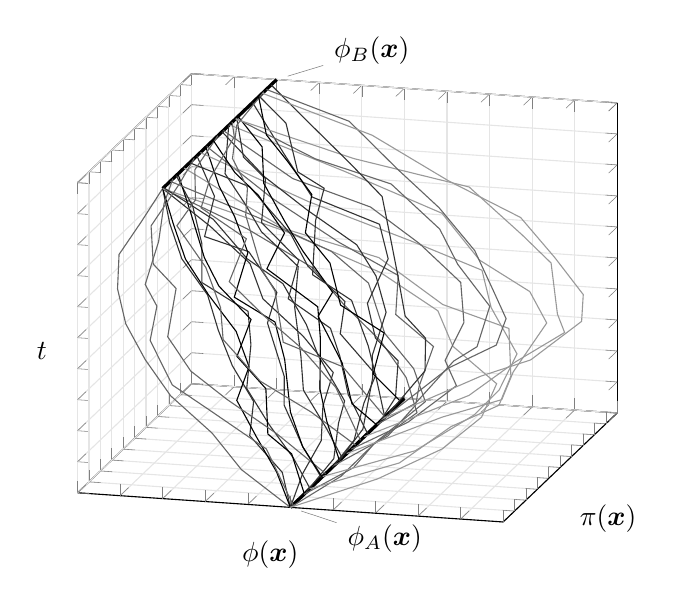
\begin{tikzpicture}
\begin{axis}[
	clip=false,
	view={-75}{20}, 
	%xtick=\empty, ytick=\empty, ztick=\empty, 
	xticklabel=\empty, yticklabel=\empty, zticklabel=\empty,
	xlabel=$\pi(\vec{x})$, ylabel=$\phi(\vec{x})$, zlabel=$t$, zlabel style={rotate=-90},
	%x label style={at={(axis description cs:0.5,0.0)},anchor=north},
	%y label style={at={(axis description cs:0.5,0.0)},anchor=north},
	%z label style={at={(axis description cs:0.5,0.0)},anchor=north},
	xmin=0, xmax=1, ymin=0, ymax=1, zmin=0, zmax=5,
	xtick distance=0.1, ytick distance=0.1, ztick distance=0.5, grid=major, grid style={solid, thin, black!10!white},
	%extra x ticks={0j
	declare function={
		phi1 = 0.5;
		phi2 = 0.8;
		randbetween(\a,\b) = \a + (\b - \a) / 2 * rand;
		%randradius(\x, \rmin, \rmax) = randbetween(\rmin, \rmax) * (\x-0) * (\x-1);
		randfunc(\x,\rmin,\rmax) = randbetween(\rmin,\rmax) * (\x-0)*(\x-1) * 4; % and(x>=0.01, x<=0.99); %(\x-0) * (\x-1);
	},
]
\addplot3 [domain=0:1, samples=2, very thick] ({x}, {phi1}, {0}) node [pos=0.0,pin={-8:$\phi_A(\vec{x})$}] {};
\addplot3 [domain=0:1, samples=2, very thick] ({x}, {phi2}, {5}) node [pos=1.0,pin={+5:$\phi_B(\vec{x})$}] {};
\pgfplotsinvokeforeach{0.0, 0.2, ..., 1.0} {
	\addplot3 [domain=0:1, samples=10, domain y=0:1, samples y=1, black!60!white]  ({max(0, min(1, #1+randbetween(-0.1,0.1))}, {phi1 + (phi2-phi1)*x + randfunc(x,-0.2,-0.3)}, {5*x});
	\addplot3 [domain=0:1, samples=10, domain y=0:1, samples y=1, black!80!white]  ({max(0, min(1, #1+randbetween(-0.1,0.1))}, {phi1 + (phi2-phi1)*x + randfunc(x,-0.0,-0.1)}, {5*x});
	\addplot3 [domain=0:1, samples=10, domain y=0:1, samples y=1, black!100!white] ({max(0, min(1, #1+randbetween(-0.1,0.1))}, {phi1 + (phi2-phi1)*x + randfunc(x,+0.0,+0.1)}, {5*x});
	\addplot3 [domain=0:1, samples=10, domain y=0:1, samples y=1, black!80!white]  ({max(0, min(1, #1+randbetween(-0.1,0.1))}, {phi1 + (phi2-phi1)*x + randfunc(x,+0.2,+0.3)}, {5*x});
	\addplot3 [domain=0:1, samples=10, domain y=0:1, samples y=1, black!60!white]  ({max(0, min(1, #1+randbetween(-0.1,0.1))}, {phi1 + (phi2-phi1)*x + randfunc(x,+0.4,+0.5)}, {5*x});
	\addplot3 [domain=0:1, samples=10, domain y=0:1, samples y=1, black!40!white]  ({max(0, min(1, #1+randbetween(-0.1,0.1))}, {phi1 + (phi2-phi1)*x + randfunc(x,+0.6,+0.7)}, {5*x});
	%\addplot3 [domain=0:1, samples=10, domain y=0:1, samples y=1] ({#1+randfunc(x,0.2,0.3)}, {phi1 + (phi2-phi1)*x + randfunc(x,0.1,0.2)}, {5*x});
}
\end{axis}
\end{tikzpicture}
\caption{\label{fig:phase_space}A quantum system that evolves from the initial field $\phi_A(\vec{x})$ to the final field $\phi_B(\vec{x})$ can take all possible paths through phase space, but some are more likely than others. The conjugate momentum field $\pi(\vec{x})$ does not need to be the same at the start and the end.}
\end{figure}

Substituting \cref{eq:tft:inner_product_position_momentum,eq:tft:path_integral_hamiltonian_assumption,eq:tft:hamiltonian_eigenvalues}, the transition amplitude \eqref{eq:tft:transition_amplitude_product} becomes
\begin{equation}
\begin{split}
	\transampl &=      \left( \prod_{n=1}^N \int \frac{\dif \phi_n \dif \pi_n}{2 \pi \hbar} \right) \\
	           &\times \exp \left( \frac{i \Delta t}{\hbar} \sum_{n=1}^N \int \dif^3 x \left( \pi_n(\vec{x}) \frac{\phi_{n+1}(\vec{x}) - \phi_n(\vec{x})}{\Delta t} - \ham(\pi_n(\vec{x}), \phi_n(\vec{x})) \right)
	\right)
\end{split}
\end{equation}
Finally, we take the continuum limit by sending $N \rightarrow \infty$.
It is then natural to define
$\phi(\vec{x}, t_n) = \phi_n(\vec{x}, t_n)$
and
$\pi(\vec{x}, t_n) = \pi_n(\vec{x}, t_n)$
to be the values of the fields at each timestep $t_n$.
Both become continuous functions of time in the continuum limit.
We also use the finite difference definition of the derivative to turn the fraction in the exponential into a partial derivative $\dot{\phi}(\vec{x},t) = \pdv{\phi(\vec{x},t)}/{t}$.
Similarly, we use the Riemann sum definition of the integral to turn the sum $\sum \Delta t$ into an integral $\int \dif t$.
We also define the \textbf{functional integrals}
\begin{equation}
	\int \pathintdif \phi = \lim_{N \rightarrow \infty} \prod_{n=1}^{N} \int \dif \phi_n
	\qquad \text{and} \qquad
	\int \pathintdif \pi = \lim_{N \rightarrow \infty} \prod_{n=1}^{N} \int \frac{\dif \pi_n}{2 \pi \hbar} .
\label{eq:tft:functional_integral}
\end{equation}
%We have swept the diverging factor $(2 \pi \hbar)^N$ under the rug, arguing that it contains no physical information about the dynamics of the process and can be ignored, unlike the other factors.
%TODO: can integrate out momentum with gaussian integral if it appears as $p^2$)
With all of these steps, the transition amplitude takes the form of the \textbf{path integral}
\begin{equation}
\begin{split}
	\transampl &=      \int \pathintdif \pi \int_{\phi(\vec{x}, 0)=\phi_A(\vec{x})}^{\phi(\vec{x},T)=\phi_B(\vec{x})} \pathintdif \phi \\
	           &\times \exp \left( \frac{i}{\hbar} \int_0^T \dif t \int \dif^3 x \left( \pi(\vec{x}, t) \dot{\phi}(\vec{x}, t) - \ham(\pi(\vec{x}, t), \phi(\vec{x}, t)) \right) \right) .
\end{split}
\label{eq:tft:path_integral_hamiltonian}
\end{equation}

It is tempting to recognize $\pi \dot\phi - \ham$ as the Legendre transformation that converts to the Lagrangian density and write $\lagr$ in its place.
But we should be careful -- the Legendre transformation converts the independent variable $\dot\phi$ in $\lagr(\phi, \dot\phi, \nabla\phi)$ to $\pi$ in $\ham(\phi, \pi, \nabla\phi)$.
We are integrating over $\pi$ and should therefore not lose track of it by writing $\lagr = \lagr(\phi, \dot\phi, \nabla\phi)$.
Thus, we do not modify the integral further.
\TODO{does this make sense?}

\TODO{write just $\ham$ etc. instead to make notation lighter, then write in text the arguments?}

\iffalse
Note that the combination of the Hamiltonian and the fields in the exponential is precisely the Legendre transformation that converts between the Hamiltonian density $\ham$ and the Lagrangian density $\lagr$.
Thus, we might as well express the transition amplitude as the \textbf{path integral}
%	\transampl = \int \pathintdif \pi \int_{\phi_A(\vec{x}, 0)}^{\phi_B(\vec{x}, T)} \pathintdif \phi \\
%	             \exp \left( i \int_0^T \dif t \int \dif^3 x \, \left( \lagr(\pi(\vec{x}, t), \phi(\vec{x}, t)) \right) \right) .
\begin{equation}
	\transampl = \int \pathintdif \pi \int_{\phi_A(\vec{x})}^{\phi_B(\vec{x})} \pathintdif \phi \, \exp \big( i S \left[ \pi(\vec{x}, t), \phi(\vec{x}, t) \right] / \hbar \big) ,
\label{eq:tft:path_integral_lagrangian}
\end{equation}
with the action
\begin{equation}
	S \left[ \pi(\vec{x}, t), \phi(\vec{x}, t) \right] = \int_0^T \dif t \int \dif^3 x \, \lagr \left( \pi(\vec{x}, t), \phi(\vec{x}, t) \right) . \qquad \text{TODO: factor $c$?}
\label{eq:tft:action}
\end{equation}
\fi
The path integral expresses the transition amplitude for the process $A \rightarrow B$ as a sum over all possible paths through phase space, each weighted by the value on the unit circle with phase corresponding to the action of the path.
This interpretation is illustrated in \cref{fig:phase_space}.
Note that the position-space integral $\int \pathintdif \phi$ is constrained to start and end in the initial and final states, but the momentum integral $\int \pathintdif \pi$ has no such constraint.

Why have we spent so much time on this transition amplitude, when we really are only interested in the partition function \eqref{eq:tft:partition_function}?
If we evaluate the trace \eqref{eq:tft:partition_function} in the basis of fields $\ket{\phi_0}$, we obtain
\begin{equation}
	Z = \int \dif \phi_0 \braket{\phi_0 | e^{-\beta (\hat{H} - \mu_i \hat{N}_i)} | \phi_0} .
\end{equation}
This is precisely an integral over transition amplitudes \eqref{eq:tft:path_integral_hamiltonian}, but now with 
\begin{itemize}
\item equal start and end states $\ket{\phi_A} = \ket{\phi_B} = \ket{\phi_0}$, 
\item the Hamiltonian $\hat{H} - \mu_i \hat{N}_i$ and 
\item a purely imaginary time variable $t = -i \tau$ with $\tau$ running from $0$ to $\beta \hbar$.
\end{itemize}
The change from a real to imaginary time variable can be accomplished by a Wick rotation that does not change the value of the integral \TODO{true?}.
Thus, we can express the partition function as path integrals \eqref{eq:tft:path_integral_hamiltonian} with these substitutions!
This yields
\TODO{clarify that $i \int \dif t \rightarrow i \int (-i) \dif \tau = 1 \int \dif \tau$ and $\dot\phi(x,t) = \pdv{\phi(x,t)}/{t} \rightarrow \pdv{\phi(x,\tau)}{-i \tau} \phi(x,\tau) = i \pdv{\phi(x,\tau)}{\tau}$?}
\begin{equation}
	Z = \int \pathintdif \pi \oint_+ \pathintdif \phi \, \exp \left( \frac{1}{\hbar} \int_0^{\beta \hbar} \dif \tau \int \dif^3 x \left( i \pi \dot{\phi} - \ham + \mu \numdensity) \right) \right)
\label{eq:tft:bosonic_partition_function}
\end{equation}
where we have absorbed $\int \dif \phi_0$ into the path integral $\int \pathintdif \phi$ and write $\oint_+$ to indicate that we integrate over all fields $\phi(x, \tau) = \phi(x, \tau + \beta \hbar)$ that are \emph{periodic} in ``imaginary time'' $\tau$, due to the equal start and end states $\phi_A(\vec{x}) = \phi_B(\vec{x})$ in \cref{eq:tft:path_integral_hamiltonian}.
Thus, thermal field theory -- statistical mechanics for quantum fields at finite temperature -- is essentially equivalent to ordinary quantum field theory with temperature-dependent time and periodic fields, and the partition function is obtained by integrating along closed paths in phase space!

We have not yet discussed the appearance of the chemical potential $\mu$ and the number density $\numdensity$ in the path integral.
If the theory admits one or more conserved conserved currents $j_i^\mu$ with $\partial_\mu j_i^\mu$ by Noether's theorem, there are associated conserved charges $Q_i = \int \dif^3 x \, j_i^0$.
For every such conserved charge, we can associate a chemical potential $\mu_i$ and include the term
\begin{equation}
	\mu_i \numdensity_i = \mu_i j_i^0
\label{eq:tft:chemical_potential}
\end{equation}
in the path integral.
For example, if the theory has particles and antiparticles, then a conserved charge typically corresponds to the difference between the number of particles and antiparticles in the system.
The chemical potential can then be interpreted as a knob with which we can regulate the balance between particles and antiparticles in the system.
We will later see examples of theories both with and without conserved charges.

\TODO{i do not understand properly how the chemical potential works and why we can include it}

\section{Path integral for fermionic partition function}

%\newcommand\creat[1]{\hat\psi^\dagger(\vec{#1})}
%\newcommand\destr[1]{\hat\psi        (\vec{#1})}
\newcommand\creat{\hat\psi^\dagger}
\newcommand\destr{\hat\psi        }

We will now develop a path integral for a fermionic field $\psi(\vec{x})$.
For example, the Dirac Lagrangian is $\lagr = \bar{\psi} (i \hbar c \slashed\partial - m c^2) \psi$ with conjugate momentum $\pi = \fdv{\lagr}/{\dot\psi} = i \hbar \psi^\dagger$, so we are instructed to treat the field and its conjugate independently in the path integral.
This is not a peculiarity of fermionic fields only -- for a complex scalar field $\phi$, for example, we would also be instructed to treat $\phi$ and $\conj\phi$ separately. 

Why do we need to derive the path integral for fermions separately -- can we not just use the bosonic path integral \eqref{eq:tft:bosonic_partition_function} with the appropriate conjugate momentum?
By assumption, the fermion field operator $\destr(\vec{x})$ and its conjugate $\creat(\vec{x})$ obey the fermionic \textbf{anticommutation relations}
\begin{equation}
\begin{split}
	\acomm{\destr(\vec{x})}{\creat(\vec{y})} = \acomm{\creat(\vec{y})}{\destr(\vec{x})} &= \delta(\vec{x}-\vec{y}) , \\
	\acomm{\creat(\vec{x})}{\creat(\vec{y})} = \acomm{\destr(\vec{x})}{\destr(\vec{y})} &= 0 ,
\end{split}
\label{eq:tft:fermion_anticommutators}
\end{equation}
in contrast to the bosonic commutators \eqref{eq:tft:boson_field_commutators}.
In the derivation of the bosonic path integral \eqref{eq:tft:bosonic_partition_function}, we treated the eigenvalues $\phi$ and $\pi$ of the operators $\hat\phi$ and $\hat\pi$ as ordinary numbers.
However, the anticommutators \eqref{eq:tft:fermion_anticommutators} of the fermionic field operators in fact requires their eigenvalues to anticommute!
For example,
\begin{equation}
\begin{split}
	\text{if}   \quad & \destr \ket{\psi} = \psi \ket{\psi} , \\
	\text{then} \quad & \braket{\psi | \creat \destr | \psi} = \braket{\psi | \conj\psi \psi | \psi} = -\braket{\psi | \psi \conj\psi | \psi} = -\braket{\psi | \destr \creat | \psi} \quad \text{by \eqref{eq:tft:fermion_anticommutators}}, \\
	\text{so}   \quad & \acomm{\psi}{\conj\psi} = 0 . \\
\end{split}
\label{eq:tft:eigenvalues_must_anticommute}
\end{equation}
By similar reasoning, one can also deduce the requirements $\acomm{\psi}{\creat} = \acomm{\psi}{\destr} = 0$.
The bosonic path integral \eqref{eq:tft:bosonic_partition_function} and its derivation is therefore not valid for fermions.

To develop the fermionic path integral, we therefore replace the algebra of ordinary commuting numbers in the bosonic case with anticommuting \textbf{Grassmann numbers}.
Assuming most readers have encountered them before, we define and derive all properties of Grassmann numbers that will be useful to us in \cref{chap:grassmann_numbers} and will only refer to them in this section.

In the derivation of the bosonic path integral \eqref{eq:tft:bosonic_partition_function}, we relied heavily on using eigenstates of the system to take the trace in \eqref{eq:tft:partition_function}, insert completeness relations and take inner products between eigenstates.
To find analogous ways of doing this with fermionic fields, we will introduce \textbf{fermionic coherent states}.

\iffalse
To compute the fermionic path integral, we must therefore replace the algebra of commuting complex numbers in the bosonic case with the algebra of anticommuting \textbf{Grassmann numbers}.
This algebra was invented by the German mathematician Hermann Grassmann in the 19th century.
His work did not gain much traction at that time.
In fact, the publisher of one of his book once wrote to him that
\emph{``(...) since your work hardly sold at all, roughly 600 copies were used in 1864 as waste paper and the remaining few odd copies have now been sold out, with the exception of the one copy in our library.''}
Grassmann was so disappointed with the reception of his work that he turned to study linguistics the last years of his life.
Today, however, his work on Grassmann numbers is the whole fundament for the construction of the fermionic path integral, and his other work is also very important \TODO{fix}.
We review Grassmann numbers in \TODO{ref appendix}.

For concreteness, consider fermions described by the Dirac Lagrangian
\begin{equation}
	\lagr = \bar{\psi} (i \hbar c \slashed\partial - m c^2) \psi .
\end{equation}
Here, the conjugate momentum turns out to be
\begin{equation}
	\pi = \fdv{\lagr}{\dot\psi} = i \hbar \psi^\dagger ,
\label{eq:tft:dirac_conjugate_momentum}
\end{equation}
so, perhaps confusingly, we are instructed to treat the field and its conjugate as independent variables in the path integral.
\fi

\TODO{take into account \url{https://physics.stackexchange.com/questions/163592/multivariable-functions-of-grassmann-numbers}, see Altland Simons ``4.5 Problems''}

Let us get to work.
Suppose we have a finite number $N$ of Grassmann numbers $\psi_i$ and equally many creation and destruction operators $\creat_i$ and $\destr_i$.
Following the discussion around \cref{eq:tft:eigenvalues_must_anticommute} and the definition of Grassmann numbers in \cref{chap:grassmann_numbers}, we have, by assumption, all the anticommutators
\begin{equation}
\begin{split}
	\acomm{\psi_i}{\psi_j} = \acomm{\psi_i}{\conj\psi_j} = \acomm{\conj\psi_i}{\conj\psi_j}                             &= 0            , \\
	\acomm{\psi_i}{\destr_j} = \acomm{\psi_i}{\creat_j} = \acomm{\conj\psi_i}{\destr_j} = \acomm{\conj\psi_i}{\creat_j} &= 0            , \\
	\acomm{\destr_i}{\destr_j} = \acomm{\creat_i}{\creat_j}                                                             &= 0            , \\
	\acomm{\destr_i}{\creat_j} = \acomm{\creat_j}{\destr_i}                                                             &= \delta_{i j} . \\
\end{split}
\label{eq:tft:fermionic_all_anticommutators}
\end{equation}
In other words, all field operators and all Grassmann numbers anticommute with themselves and each other.
The anticommutators \eqref{eq:tft:fermionic_all_anticommutators} of the field operators $\creat_i$ and $\destr_i$ are the discrete analogues of \eqref{eq:tft:fermion_anticommutators}.
It will be less painful to describe the formalism of fermionic coherent states in the discrete case and then take the continuum limit $\psi_i \rightarrow \psi(\vec{x})$ in the end.

The Fock space of the fermionic field has a \textbf{ground state} or \textbf{vacuum state} that we denote by
\begin{equation}
	\ket{0, 0, \ldots, 0} = \ket{0}. \\
\end{equation}
We can apply any sequence of $n = \sum_i n_i$ different creation operators to it to build an \textbf{$n$-particle state}
\begin{equation}
	\ket{n_1, n_2, \ldots, n_N} = \left( \creat_1 \right)^{n_1} \cdots \left( \creat_N \right)^{n_N} \ket{0} .
\label{eq:tft:fermionic_many_particle_state}
\end{equation}
This results in a non-zero state only if $n_i \in \{0, 1\}$ for all $i$, because $(\creat_i)^2 \ket{0} = -(\creat_i)^2 \ket{0} = 0$ by the anticommutator \eqref{eq:tft:fermionic_all_anticommutators}.
Note that shuffling the sequence of operators in \cref{eq:tft:fermionic_many_particle_state} can change the sign -- we define the $n$-particle state to have operators with indices that increase from left to right.
In particular, we can build the \textbf{one-particle state}
\begin{equation}
	\ket{1_i} = \ket{(n_1=0), \ldots, (n_i=1), \ldots, (n_N=0)} = \creat_i \ket{0} .
\end{equation}
Note also that $\creat_i \ket{1_i} = (\creat_i)^2 \ket{0} = -(\creat_i)^2 \ket{0} = 0$.
Therefore we have
\begin{equation}
	\destr_i \ket{1_i} = \destr_i \creat_i \ket{0} = (1 - \creat_i \destr_i) \ket{0} = \ket{0} .
\end{equation}
The interpretation of this analysis is that the \textbf{creation operator} $\creat_i$ adds a particle in the state $i$, while the \textbf{destruction operators} $\destr_i$ removes a particle from the same state.
The restriction that $n_i \in \{0, 1\}$ implies that there can be at most one particle in every state, consistent with the Pauli exclusion principle.
Note that the Fock space has a total of $2^N$ distinct states
\begin{equation}
	\ket{n_1, n_2, \ldots, n_N} \qquad \text{where } n_i \in \{0, 1\} \text{ for all } i = 1, \ldots, N .
\label{eq:tft:fermion_all_states}
\end{equation}

Next, define the \textbf{coherent state}
\begin{equation}
	\ket{\psi} = \exp \left( -\sum_i \psi_i \creat_i \right) \ket{0} = \prod_i \exp \left( -\psi_i \creat_i \right) \ket{0} = \prod_i \left( 1 - \psi_i \creat_i \right) \ket{0} .
\end{equation}
In the last line, we made use of the Taylor expansion \eqref{eq:gnums:function_taylor_series} of functions of Grassmann numbers.
Applying a destruction operator to this state gives
\begin{equation}
\begin{aligned}
	%\destr_j \ket{\psi} = \psi_j \ket{0} = \psi_j \ket{\psi} \quad \text{(last because $\psi_j^2=0$)}
	%\destr_j \ket{\psi} = \destr_j \prod_i \left( 1 - \psi_i \creat_i \right) \ket{0} = + \psi_j \destr_j \creat_j \ket{0} = \psi_j \ket{0} .
	\destr_j \ket{\psi} &= \destr_j \prod_i \left( 1 - \psi_i \creat_i \right) \ket{0} = \prod_{i \neq j} \left( 1 - \psi_i \creat_i \right) \destr_j \left( 1 - \psi_j \creat_j \right) \ket{0} \\
	                    &= \prod_{i \neq j} \left( 1 - \psi_i \creat_i \right) \psi_j \ket{0} = \prod_{i \neq j} \left( 1 - \psi_i \creat_i \right) \psi_j \left( 1 - \psi_j \creat_j \right) \ket{0}   \\
	                    &= \psi_j \prod_i \left( 1 - \psi_i \creat_i \right) \ket{0} = \psi_j \ket{\psi} . \\
\end{aligned}
\end{equation}
In other words, the coherent state $\ket{\psi}$ is an eigenstate of every destruction operator $\destr_j$ with eigenvalue $\psi_j$!
This is analogous to the bosonic eigenequation \eqref{eq:tft:field_eigenvalue_equations}.
It is the coherent states that we wish to use when taking the trace, inner product and inserting identity operators in the path integral.

First, let us find the inner product between two coherent states.
It is
\begin{equation}
\begin{split}
	\iffalse
	\braket{\psi | \psi'} &= \braket{0 | \prod_i (1 - \destr_i \conj\psi_i) \prod_j (1 - \psi'_j \creat_j) | 0} \\
	                      &= \braket{0 | 0} + \sum_{i,j} \braket{0 | \destr_i \conj\psi_i \psi'_j \creat_j | 0}
	                       = \braket{0 | 0} + \sum_{i,j} \conj\psi_i \psi'_j \braket{0 | \destr_i \creat_j | 0} \\
	                      &= \braket{0 | 0} + \sum_{i  } \conj\psi_i \psi'_i
						   = 1 + \sum_i \conj\psi_i \psi'_i = \exp \left( \sum_i \conj\psi_i \psi'_i \right) .
	\fi
	\braket{\psi | \psi'} &= \braket{\psi | \prod_i (1 - \psi'_i \creat_i) | 0} = \braket{\psi | \prod_i (1 + \creat_i \psi'_i) | 0} = \braket{\psi | \prod_i (1 + \conj\psi_i \psi'_i) | 0} \\
						  &= \underbrace{\braket{0 | 0}}_{1} \prod_i (1 + \conj\psi_i \psi'_i) = \prod_i \exp(\conj\psi_i \psi'_i) = \exp \left( \sum_i \conj\psi_i \psi'_i \right) .
\end{split}
\label{eq:tft:grassmann_inner_product_discrete}
\end{equation}

Next, we can work out that the unit operator $\hat{1}$ can be represented by the integral
\begin{equation}
\begin{split}
	 \iffalse
	 & \int \dif \conj{\psi} \int \dif \psi \, e^{-\sum_i \conj\psi_i \psi_i} \ket{\psi} \bra{\psi} \\
	=& \int \dif \conj{\psi} \int \dif \psi \, \prod_i \left( 1 + \psi_i \conj{\psi}_i \right) \prod_j \left( 1 - \psi_j \creat_j \right) \ket{0} \bra{0} \prod_k \left( 1 - \destr_k \conj\psi_k \right) \\
	=& \int \dif \conj{\psi} \int \dif \psi \, \prod_i \left( 1 + \psi_i \conj{\psi}_i \right) \prod_j \left( 1 - \psi_j \creat_j \right) \ket{0} \bra{0} \left( 1 - \destr_j \conj\psi_j \right) \\
	=& \sum_{n_1=0}^1 \sum_{n_2=0}^1\cdots \sum_{n_N=0}^1 \ket{n_1, n_2, \ldots, n_N} \bra{n_1, n_2, \ldots, n_N} = \hat{1} \\
	=& \int \dif \conj{\psi} \int \dif \psi \left[ \left( -\sum_i \conj{\psi}_i \psi_i \right) \ket{0} \bra{0} + \left( -\sum_j \psi_j \creat_j \right) \ket{0} \bra{0} \left( -\sum_k \destr_k \conj\psi_k \right) \right] \\
	=& \int \dif \conj{\psi} \int \dif \psi \left[ \sum_i \psi_i \conj\psi_i \ket{0} \bra{0} + \sum_{j,k} \psi_j \conj\psi_k \ket{1_j} \bra{1_k} \right] \\
	=& \ket{0} \bra{0} + \sum_j \ket{1_j} \bra{1_j} = \hat{1} . \\
	\fi
	 & \int \dif \conj{\psi} \int \dif \psi \, \exp \left( -\sum_i \conj\psi_i \psi_i \right) \ket{\psi} \bra{\psi} \\
	=& \int \dif \conj{\psi} \int \dif \psi \, \prod_i \left( 1 + \psi_i \conj{\psi}_i \right) \prod_j \left( 1 - \psi_j \creat_j \right) \ket{0} \bra{0} \prod_k \left( 1 - \destr_k \conj\psi_k \right) \\
	=& \sum_{n_1=0}^1 \sum_{n_2=0}^1\cdots \sum_{n_N=0}^1 \ket{n_1, n_2, \ldots, n_N} \bra{n_1, n_2, \ldots, n_N} = \hat{1} . \\
\end{split}
\label{eq:tft:completeness_grassmann_discrete}
\end{equation}
To make the big leap across the second equality sign, stare intensely at the middle line as you follow the next argument.
To get a non-zero contribution from the integral, the parentheses must be multiplied out in a way such that one gets terms with the particular combination
\begin{equation}
	\int \dif \conj\psi \int \dif \psi \, \psi_1 \conj\psi_1 \cdots \psi_N \conj\psi_N = 1 .
\label{eq:tft:integral_saturated}
\end{equation}
Any term with duplicate fields $\psi_i^2 = -\psi_i^2 = 0$ will yield zero, and so will terms with products that do not include \emph{all} $\psi_i$ and $\conj\psi_i$ due to the integration properties \eqref{eq:gnums:integration_differentiation} and the discussion surrounding \cref{eq:gnums:integration_over_all}.
Based on this, we can derive three rules for what combinations of factors we can choose when multiplying out the three parentheses.
\begin{enumerate}
\item \textbf{For any $i$ in the first parenthesis:} We are free to choose either the factor $1$ or $\psi_i \conj\psi_i$. \label{eq:tft:logic_tree_one}
\item \textbf{For $j=i$ in the second parenthesis:} 
If we choose $\psi_i \conj\psi_i$ in the first parenthesis, we \emph{must} choose $1$ in the second to avoid a duplicate factor $\psi_i^2 = 0$.
Conversely, if we choose $1$ in the first, we \emph{must} choose $-\psi_j \creat_j$ in the second to ``saturate'' the field product.
\item \textbf{For $k = j = i$ in the third parenthesis:} 
If we choose $-\psi_j \creat_j$ in the second, we \emph{must} choose $-\psi_k \creat_k$ in the third to get $\psi_j \conj\psi_j$ in the field product.
Conversely, if we choose $1$ in the second, then we have already included $\psi_i \conj\psi_i$ from rule \ref{eq:tft:logic_tree_one}, and we \emph{must} choose $1$ in the third to not ``oversaturate'' the field product.
\end{enumerate}
Following these rules, the first parenthesis expands to all possible $2^N$ terms.
For every one of these terms, there is precisely one legal combination of factors to choose in the second and third parentheses.
This evaluates to $2^N$ terms with all possible combinations of $N_j = N_k$ creation and annihilation operators and $N_i = N - N_j$ Grassmann numbers.
\emph{These $2^N$ terms are therefore precisely all the $2^N$ states \eqref{eq:tft:fermion_all_states} in the system!}
This explains the transition to the final line.
\iffalse
\begin{itemize}
\item choose $k = j$ in the third parenthesis in order to pair $\psi_j$ with $\conj\psi_j$, and
\item for every factor $\psi_i \conj\psi_i$ one chooses from the first parenthesis, one must choose the factor $1$ from the second and third parentheses in order to avoid $\psi_i^2=0$, and conversely,
\item for every factor $1$ one chooses from the first parenthesis, one must choose the factor $-\psi_j \creat_j$ and $-\destr_k \conj\psi_k$ from the second and third parentheses in order to not miss a factor $\psi_i \conj\psi_i$ in the product \TODO{ref}.
\end{itemize}
Following these rules is equivalent to iterating over all $2^N$ combinations with $N_j$ creation and destruction operators in the second and third parentheses and $N_i = N - N_j$ Grassmann numbers in the first parenthesis.
\fi
To be clear, the very last equality follows because the sum goes over all states \eqref{eq:tft:fermion_all_states} in the system.

With the same reasoning, we can work out that the trace of an operator $\hat{A}$ can be written
\begin{equation}
\begin{split}
	 & \int \dif \conj{\psi} \int \dif \psi \, \exp \left( -\sum_i \conj{\psi}_i \psi_i \right) \braket{-\psi | \hat{A} | \psi} \\
	=& \int \dif \conj{\psi} \int \dif \psi \, \prod_i (1 + \conj\psi_i \psi_i) \braket{0 | \prod_j (1 + \destr_j \conj\psi_j) \hat{A} \prod_k (1 - \psi_k \creat_k) | 0} \\
	=& \int \dif \conj{\psi} \int \dif \psi \, \prod_i (1 + \conj\psi_i \psi_i) \braket{0 | \prod_j (1 + \destr_j \conj\psi_j) \hat{A} (1 - \psi_j \creat_j) | 0} \\
	%=& \int \dif \conj{\psi} \int \dif \psi \, \prod_i (1 + \conj\psi_i \psi_i) \prod_j \conj\psi_j \psi_j \braket{0 | (1 + \destr_j \psi_j) \hat{A} (1 + \conj\psi_j \creat_j) | 0} \\
	=& \sum_{n_1=0}^1 \sum_{n_2=0}^1\cdots \sum_{n_N=0}^1 \braket{n_1, n_2, \ldots, n_N | \hat{A} | n_1, n_2, \ldots, n_N} = \trace{\hat{A}} . \\
	%=& \int \dif \conj{\psi} \int \dif \psi \left[ (-\sum_i \conj\psi_i \psi_i) \braket{0 | \hat{A} | 0} + \braket{0 | (+\sum_j \destr_j \conj\psi_j) \hat{A} (-\sum_k \psi_k \creat_k) | 0} \right] \\
	%=& \int \dif \conj{\psi} \int \dif \psi \left[ \sum_i \psi_i \conj\psi_i \braket{0 | \hat{A} | 0} + \sum_{j,k} \psi_k \conj\psi_j \braket{1_j | \hat{A} | 1_k} \right] \\
	%=& \braket{0 | \hat{A} | 0} + \sum_j \braket{1_j | \hat{A} | 1_j} = \trace{\hat{A}} . \\
\end{split}
\label{eq:tft:trace_grassmann_discrete}
\end{equation}
Across the third equality, we (anti)commute $\psi_j$ and $\conj\psi_j$ all the way to the left to write $\braket{0 | \destr_j \conj\psi_j \hat{A} (-\psi_j \creat_j) | 0} = \psi_j \conj\psi_j \braket{0 | \destr_j \hat{A} \creat_j | 0}$ while assuming that $\hat{A}$ is a ``bosonic'' operator that \emph{commutes} with the Grassmann numbers.
The Hamiltonian \eqref{eq:tft:dirac_hamiltonian} for a Dirac field that we encounter later is one example of such an $\hat{A}$, as it contains two field operators.

As we remarked at the start, this analysis was for discrete fields that satisfies the discrete anticommutators \eqref{eq:tft:fermionic_all_anticommutators}.
We are studying fields $\psi(\vec{x})$ and $\conj\psi(\vec{x})$ with an infinite number of field operators $\creat(\vec{x})$ and $\destr(\vec{x})$ that satisfy the continuum generalization \eqref{eq:tft:fermion_anticommutators}.
Our results carry over with the substitutions $\psi_i \rightarrow \psi(\vec{x})$, as if every Grassmann number corresponds to the field at one position, and $\sum_i \rightarrow \int \dif^3 x$.
For example, we would rather define the coherent state
\begin{equation}
	\ket{\psi} = \exp \left( -\int \dif^3 x\, \psi(\vec{x}) \hat\psi^\dagger(\vec{x}) \right) \ket{0} .
\end{equation}
The inner product \eqref{eq:tft:grassmann_inner_product_discrete} between two coherent states would then become
\begin{equation}
	\braket{\psi | \psi'} = \exp \left( \int \dif^3 x \, \conj\psi(\vec{x}) \psi'(\vec{x}) \right)
\label{eq:tft:grassmann_inner_product}
\end{equation}
The identity operator \eqref{eq:tft:grassmann_inner_product_discrete} would then become
\begin{equation}
	\int \dif \conj\psi \int \dif \psi \, \exp \left( -\int \dif^3 x \, \conj\psi(\vec{x}) \psi(\vec{x}) \right) \ket{\psi} \bra{\psi} = \hat{1} ,
\label{eq:tft:completeness_grassmann}
\end{equation}
while the trace \eqref{eq:tft:trace_grassmann_discrete} would turn out to be
\begin{equation}
	\int \dif \conj\psi \int \dif \psi \, \exp \left( -\int \dif^3 x \, \conj\psi(\vec{x}) \psi(\vec{x}) \right) \braket{-\psi | \hat{A} | \psi} = \trace{A} .
\label{eq:tft:trace_grassmann}
\end{equation}
The most important thing to note is the negative sign in $\bra{-\psi}$ of the trace \eqref{eq:tft:trace_grassmann} -- we will see that this requires fermionic fields to be \emph{antiperiodic} in imaginary time, in contrast to the periodic bosonic fields.

The partition function \eqref{eq:tft:partition_function} follows from the trace \eqref{eq:tft:trace_grassmann} with $\hat{A} = e^{-\beta (\hat{H} - \mu \hat{N})}$ as
\begin{equation}
	Z = \int \dif \psi_0^\dagger \int \dif \psi_0 \, e^{-\int \dif^3 x \, \psi_{0}^\dagger(\vec{x}) \psi_{0}(\vec{x})} \braket{-\psi_0 | e^{-\beta(\hat{H} - \mu \hat{N})} | \psi_0} .
\end{equation}
Breaking up the operator $e^{\ldots}$ as in \cref{eq:tft:time_evolution_splitting} and inserting one Grassmann completeness relation \eqref{eq:tft:completeness_grassmann} between every factor, the partition function becomes
\begin{equation}
	Z = \prod_n \int \dif \psi_n^\dagger \int \dif \psi_n \, e^{-\int \dif^3 x \, \psi_{n}^\dagger(\vec{x}) \psi_{n}(\vec{x})} \braket{\psi_{n+1} | e^{-(\hat{H} - \mu \hat{N}) \Delta \tau / \hbar} | \psi_n} ,
\end{equation}
where we define $\bra{\psi_{N+1}} = \bra{-\psi_0}$ -- \emph{note the minus sign!}
Next, expand the Hamiltonian to first order as in \cref{eq:tft:path_integral_hamiltonian_assumption}.
Then we obtain
\begin{equation}
	Z = \prod_n \int \dif \psi_n^\dagger \int \dif \psi_n \, e^{-\int \dif^3 x \, \psi_{n}^\dagger(\vec{x}) \psi_{n}(\vec{x})} \braket{\psi_{n+1} | \psi_n} e^{-(H_n - \mu N) \Delta \tau / \hbar} .
\end{equation}
Now use the Grassmann inner product \eqref{eq:tft:grassmann_inner_product} to write
\begin{equation}
	Z = \prod_n \int \dif \psi_n^\dagger \int \dif \psi_n \, \exp \left\{ \frac{\Delta \tau}{\hbar} \sum_n \int \dif^3 x \left( \hbar \frac{\psi^\dagger_{n+1} - \psi^\dagger_n}{\Delta \tau} \psi_{n} - \ham + \mu \numdensity \right) \right\} .
\end{equation}
Finally, take the continuum limit and integrate $\int \dif \tau \, \dot{\psi^\dagger} \psi = -\int \dif \tau \, \psi^\dagger \dot{\psi}$ by parts \TODO{why is this valid for Grassmann numbers? Can one e.g. show that $\pdv{\phi^\dagger \phi}{\tau} = 0$?, change order/use int by parts correctly}.
As in \eqref{eq:tft:functional_integral}, introduce the functional integrals $\pathintdif \psi = \lim_{N \rightarrow \infty} \prod_n \dif \psi_n$ and $\pathintdif [i \hbar \psi^\dagger] = \lim_{N \rightarrow \infty} \prod_n \psi^\dagger$, where we absorb some physically irrelevant prefactors into the latter to preserve similarity between the conjugate momentum $\pi$ and $i \hbar \psi^\dagger$. 
We then obtain the \textbf{fermionic partition function}
\begin{equation}
	Z = \oint_- \pathintdif [i \hbar \psi^\dagger] \oint_- \pathintdif \psi \exp \left\{ \frac{1}{\hbar} \int_0^{\beta \hbar} \dif \tau \int \dif^3 x \left( -\hbar \psi^\dagger \dot{\psi} - \ham ( \psi^\dagger, \psi ) + \mu \numdensity \right) \right\} ,
\label{eq:tft:fermion_partition_function}
\end{equation}
where $\oint_-$ means to integrate over \emph{antiperiodic} fields $\psi(\vec{x}, 0) = -\psi(\vec{x}, \beta \hbar)$, naturally extending the symbol $\oint_+$ we introduced for bosonic fields that were \emph{periodic}.
Apart from the difference in periodicity, this result is -- remarkably -- exactly the same as the bosonic partition function \eqref{eq:tft:bosonic_partition_function}, with canonical momentum \eqref{eq:tft:dirac_conjugate_momentum}!
But the similarity in facade were achieved by a drastically different mathematical fundament.

\TODO{do for general $\psi \rightarrow \eta$ as in random note 1 on the web, then specialize later to Dirac?}

\iffalse
The partition function is therefore
\begin{equation}
\begin{split}
	Z &= \int \dif \psi_0^\dagger \int \dif \psi_0 \, e^{-\psi_{n+1}^\dagger \psi_{n+1}} \braket{-\psi_0 | e^{-\beta(\hat{H} - \mu \hat{N})} | \psi_0} \\
	  &= \prod_n \int \dif \psi_n^\dagger \int \dif \psi_n \, e^{-\psi_{n+1}^\dagger \psi_{n+1}} \braket{\psi_{n+1} | e^{-(\hat{H} - \mu \hat{N}) \Delta \tau / \hbar} | \psi_n} \\
	  &= \prod_n \int \dif \psi_n^\dagger \int \dif \psi_n \, e^{-\psi_{n+1}^\dagger \psi_{n+1}} \braket{\psi_{n+1} | \psi_n} e^{-(H_n - \mu N) \Delta \tau / \hbar} \\
	  &= \prod_n \int \dif \psi_n^\dagger \int \dif \psi_n \, \exp \left\{ -\frac{\Delta t}{\hbar} \sum_n \int \dif^3 x \left( \psi^\dagger_{n+1} \frac{\psi_{n+1} - \psi_n}{\Delta t} + \ham - \mu \numdensity \right) \right\} \\
	  &= \oint_- \pathintdif \psi^\dagger \oint_- \pathintdif \psi \exp \left\{ \frac{1}{\hbar} \int_0^{\beta \hbar} \dif \tau \int \dif^3 x \left( -\psi^\dagger(\vec{x},\tau) \dot{\psi}(\vec{x},\tau) - \ham \left( \psi^\dagger(\vec{x},\tau), \psi(\vec{x},\tau) \right) + \mu \numdensity \right) \right\} \\
\end{split}
\end{equation}
\fi

\section{Matsubara frequencies}

We have just seen how the partition function for bosons can be expressed by the path integral \eqref{eq:tft:bosonic_partition_function} with fields that are periodic in imaginary time.
For Dirac fermions, we have showed that we can ``naively'' use the same result by substituting the canonical momentum $\pi = i \hbar \psi^\dagger$ and integrate over antiperiodic fields.
In summary, the field $\psi(\vec{x}, \tau)$ -- here regarded as \emph{either} a bosonic or fermionic field -- satisfies the (anti)periodicity
\begin{equation}
	\phi(\vec{x}, \tau) = \begin{cases}
						      + \phi(\vec{x}, \tau + \beta \hbar) & \text{for bosons} \\
						      - \phi(\vec{x}, \tau + \beta \hbar) & \text{for fermions} .
	                      \end{cases}
\label{eq:tft:periodicity}
\end{equation}
Accordingly, we can expand either field in a Fourier series
\begin{equation}
	\psi(x, \tau) = \sum_n \psi_n(x) e^{i \omega_n \tau}
\end{equation}
with \textbf{Matsubara frequencies} 
\begin{equation}
	\omega_n = \begin{cases}
			       2 \pi n / \beta \hbar    & \text{for bosons} \\
				   2 \pi (n+\frac12) / \beta \hbar & \text{for fermions} .
	           \end{cases}
\label{eq:tft:matsubara_frequencies}
\end{equation}
The offset $+\pi / \beta \hbar$ makes the fermionic field antiperiodic at $\tau = \beta \hbar$.

Although the field is not periodic in space, we can still represent it by its Fourier transform as
\begin{equation}
	\psi_n(x) = \int \frac{\dif^3 k}{(2 \pi / L)^3} \, \psi_n(\vec{k}) e^{i \vec{k} \cdot \vec{x}},
\label{eq:tft:mathematical_fourier_expansion}
\end{equation}
where $L \rightarrow \infty$ is the ``periodicity'' of the field along either axis that is sent to infinity in the Fourier transform, and $V = L^3 \rightarrow \infty$ the corresponding volume.
It will be important to have a ficticious finite volume to work with when we want to convert ``extensive'' observables like the energy $\thermalavg{E}$ into ``intensive'' observables like the energy \emph{density} $\epsilon = \thermalavg{E} / V$ in preparation for using the TOV equation \eqref{eq:tov}.
\TODO{say that $\phi_n(x)$ is periodic in $\vec{x}$ or $V$ instead (``(periodic) quantization volume''), then take $V \rightarrow \infty$}
\TODO{use bold vector on $x \rightarrow \vec{x}$ everywhere?}

Ultimately, then, we can expand
\begin{equation}
	\psi(x, \tau) = \sum_n \sum_\vec{k} \psi_n(\vec{k}) e^{i (\vec{k} \cdot \vec{x} + \omega_n \tau)}
\label{eq:tft:fourier_series}
\end{equation}
with the Matsubara frequencies \eqref{eq:tft:matsubara_frequencies}.
To be more compatible with the notation that will follow, we write
\begin{equation}
	V \int \frac{\dif^3 k}{(2 \pi)^3} = \sum_\vec{k}
\label{eq:tft:continuum_limit}
\end{equation}
with a normal summation sign, but really mean the integral in \eqref{eq:tft:mathematical_fourier_expansion}.

The wave number $\vec{k}$ and the Matsubara frequency $\omega_n$ here arose due to geometrical considerations of the periodicity of the field.
Later on, we will see that they have important physical consequences.
In anticipation of this, we define the corresponding momentum and Matsubara energy
\begin{equation}
	\vec{p} = \hbar \vec{k}, \qquad
	E_n = \hbar \omega_n \qquad \text{and} \qquad
	\sum_\vec{p} = \sum_\vec{k} = V \int \frac{\dif^3 p}{(2 \pi \hbar)^3}.
\label{eq:tft:matsubara_energies}
\end{equation}

\section{Partition function for free bosonic real scalar field}

\TODO{do Bose-Einstein with complex scalar field instead of real scalar field for more ``symmetry'' to the fermionic case?}

As a first example, we apply the path integral formalism to find the partition function for a free real scalar field representing spin-zero bosons.
Its Lagrangian density is
% note: unit of phi is sqrt(energy / length)
\begin{equation}
	\lagr = \frac{1}{2} (\partial_\mu \phi) (\partial^\mu \phi) - \frac12 \frac{m^2 c^2}{\hbar^2} \, \phi^2
	      = \frac{1}{2 c^2} \dot{\phi}^2 - \frac12 (\nabla \phi)^2  - \frac12 \frac{m^2 c^2}{\hbar^2} \, \phi^2 .
\label{eq:tft:boson_lagrangian}
\end{equation}
The conjugate momentum \TODO{ref some general formula?} is
\begin{equation}
	\pi = \pdv{\lagr}{\dot{\phi}} = \frac{1}{c^2} \dot{\phi} .
\end{equation}
The Hamiltonian density is therefore
\begin{equation}
	\ham = \pi \dot{\phi} - \lagr = \frac12 c^2 \pi^2 + \frac12 (\nabla \phi)^2 + \frac12 \frac{m^2 c^2}{\hbar^2} \phi^2 .
\label{eq:tft:boson_hamiltonian}
\end{equation}
We now calculate the partition function \eqref{eq:tft:bosonic_partition_function}.
To do so, we need the combination
\begin{equation}
\begin{split}
	i \pi \dot\phi - \ham &= i \pi \dot\phi - \frac{1}{2} c^2 \pi^2 - \frac12 (\nabla \phi)^2 - \frac{1}{2} \frac{m^2 c^2}{\hbar^2} \phi^2 \\
	                      &= -\frac{1}{2} c^2 \left( \pi - \frac{i}{c^2} \dot\phi \right)^2 - \frac{1}{2 c^2} \dot\phi^2 - \frac{1}{2} (\nabla \phi)^2 - \frac{1}{2} \frac{m^2 c^2}{\hbar^2} \phi^2 \\
	                      &= -\frac{1}{2} c^2 \tilde\pi^2 + \lagr_E . \\
\end{split}
\label{eq:tft:boson_field_combination}
\end{equation}
We completed the square by defining the shifted field $\tilde\pi = \pi - i \dot\phi / c^2$, for reasons that soon will be apparent.
Remember that the Legendre transformation \eqref{eq:tft:boson_hamiltonian} exchanges the independent variable $\dot\phi$ in $\lagr = \lagr(\phi, \dot\phi, \nabla\phi)$ to $\pi$ in $\ham = \ham(\phi, \pi, \nabla\phi)$.
Thus, the shift can be regarded as a shift by a \emph{constant}.
We also defined the remaining terms as the Lagrangian density $\lagr_E$.
It is exactly the original Lagrangian density \eqref{eq:tft:boson_lagrangian}, only with $\tau \rightarrow i \tau$.
\TODO{``correct'' if we always use $\tau$ as time variable. Make more clear by saying that the initial field is a function of $t$, then let $t \rightarrow i \tau$ and define $\tau$ as the new time variable, with e.g. $\dot f = \pdv{f}/{\tau}$?}
This can be interpreted as a change from Minkowski space to Euclidean space, and we therefore call $\lagr_E(\tau) = \lagr(i \tau)$ the Euclidean Lagrangian density.
The path integral \eqref{eq:tft:bosonic_partition_function} is then
\begin{equation}
	Z = \int \pathintdif \pi \oint_+ \pathintdif \phi \exp \left\{ \frac{1}{\hbar} \int_0^{\beta \hbar} \dif \tau \int \dif^3 x \left[ - \frac12 c^2 \tilde\pi^2 + \lagr_E \right] \right\} .
\end{equation}
Since $\tilde\pi$ can be regarded as a constant shift of the field $\pi$, we can now exploit that $\int \pathintdif \tilde\pi = \int \pathintdif \pi$ and then \emph{integrate out} the momentum using the Gaussian integral $\int_{-\infty}^{+\infty} \dif x \, e^{-x^2} = \sqrt{\pi}$ with a suitable rescaling of $x$ (where $\pi \approx 3.1415$, of course -- not the conjugate momentum).
We do not bother keeping track of this constant or any other constants in front of the partition function, as the physical quantities only involve derivatives of the logarithm of $Z$.

\TODO{ref. integral?}

\TODO{but the pressure contains $\log Z$, not a derivative, so we should not drop terms! is the resolution that, in the end, assuming all ``ghosted terms'' are infinites, we can fix it by cherry picking the non-divergent term for the pressure?}

Thus it only remains to tackle the $\phi$-integral
\begin{equation}
	Z = \oint_+ \pathintdif \phi \exp \left\{ \frac{S_E}{\hbar} \right\} ,
\label{eq:tft:boson_partition_function_momentum_out}
\end{equation}
with the Euclidean action
\begin{equation}
\begin{split}
	S_E &= \int_0^{\beta \hbar} \dif \tau \int \dif^3 x \, \lagr_E \\
	    &= \int_0^{\beta \hbar} \dif \tau \int \dif^3 x \left[ - \frac{1}{2c^2} \pdv{\phi}{\tau}^2 - \frac12 (\nabla \phi)^2 - \frac12 \frac{m^2 c^2}{\hbar^2} \phi^2 \right] .
	   %= \int_0^{\beta \hbar} \dif \tau \int \dif^3 x \, \phi \left[ \frac{1}{2c^2} \pdv[2]{}{\tau} + \frac12 \nabla^2 - \frac12 \frac{m^2 c^2}{\hbar^2} \right] \phi .
\end{split}
\label{eq:tft:boson_euclidean_action_definition}
\end{equation}
The action has no variation on the boundaries, so we can integrate by parts to convert $\pdv{\phi}/{\tau}^2$ into $-\phi \pdv[2]{\phi}/{\tau}$ and forget the boundary term.
It then becomes
\begin{equation}
	S_E = \frac12 \int_0^{\beta \hbar} \dif \tau \int \dif^3 x \, \phi \left[ \frac{1}{c^2} \pdv[2]{}{\tau} + \nabla^2 - \frac{m^2 c^2}{\hbar^2} \right] \phi .
\label{eq:tft:boson_euclidean_action_nice}
\end{equation}
\TODO{make a ``checkpoint'' here by noting that the partition function can always be written as a functional determinant, so always restart here instead of restarting the game every time}

At this point it is useful to Fourier expand the field as in \eqref{eq:tft:fourier_series} with bosonic Matsubara frequencies \eqref{eq:tft:matsubara_frequencies}.
However, we include a prefactor and write
\begin{equation}
\begin{split}
	\phi(\vec{x}, \tau) & = \hbar c \, \sqrt{\frac{\beta}{V}} \sum_{n=-\infty}^{+\infty} \sum_{\vec{k}}       \phi_n(\vec{k})  e^{+i (\vec{k} \cdot \vec{x} + \omega_n \tau)} \\
	                    & = \hbar c \, \sqrt{\frac{\beta}{V}} \sum_{n=-\infty}^{+\infty} \sum_{\vec{k}} \conj{\phi_n(\vec{k})} e^{-i (\vec{k} \cdot \vec{x} + \omega_n \tau)} ,
\end{split}
\label{eq:tft:boson_fourier_series}
\end{equation}
The prefactor $\hbar c \sqrt{\beta/V}$ is chosen to have the same dimension as the field $\phi(\vec{x}, \tau)$, so the Fourier amplitudes $\phi_n(\vec{k})$ are dimensionless.
Without it, the Gaussian integral that we will end up computing in \cref{eq:tft:boson_gaussian_integral} would make the partition function $Z$ dimensionful, which would formally make it meaningless to take its logarithm.
Note that either of the two expansions we have written is as good as the other, since the we have assumed a \emph{real} scalar field $\psi(\vec{x},\tau) = \psi(\vec{x},\tau)^*$.
\TODO{put $*$ before $($, same with powers in later functions}

\TODO{better argument for prefactor?}

\TODO{below: use $p = (p^0, \vec{p}) = (E/C, \vec{p})$ ?}

In Fourier space, then, the Euclidean action \eqref{eq:tft:boson_euclidean_action_nice} becomes
\TODO{ref to Fourier conventions to show that we only get factor $V$ etc.}
\begin{equation}
\begin{split}
	S_E & = -\frac12 \frac{\hbar^2 c^2 \beta}{V}
	        \sum_{n,n'} \sum_{\vec{k},\vec{k'}} 
	    	  \phi_{n'}(\vec{k'}) 
	    	  \left[ \frac{\omega_n^2}{c^2} + \vec{k}^2 + \frac{m^2 c^2}{\hbar^2} \right] 
	  	  \phi_{n}(\vec{k})
	  	  \underbrace{\int \dif^3 x \, e^{i (\vec{k} - \vec{k'}) \cdot \vec{x}}}_{\delta(\vec{k}-\vec{k'}) V}
	      \underbrace{\int_0^{\beta \hbar} \dif \tau \, e^{i (\omega_n - \omega_n') \tau}}_{\delta_{n,n'} \beta \hbar}
	  	  \\
	    & = -\frac12 \hbar \beta^2
	        \sum_n \sum_\vec{p}
	  	    \left[ E_n^2 + E(\vec{p})^2 \right] 
		    \abs{\phi_{n}(\vec{p})}^2 ,
\end{split}
\end{equation}
where we defined the Matsubara energies $E_n = \hbar \omega_n$ and the relativistic dispersion relation $E(\vec{p}) = \sqrt{\vec{p}^2 c^2 + m^2 c^4}$.
As we insert this action into the path integral \eqref{eq:tft:boson_partition_function_momentum_out}, it factors into the Gaussian integrals
\begin{equation}
\begin{split}
	Z & =
	\prod_{n} \prod_{\vec{p}}
	\int \dif \phi_n(\vec{p}) \,
	\exp \left[
		-\frac12 \beta^2 \left(
			E_n^2 + E(\vec{p})^2
		\right)
		\abs{\phi_n(\vec{p})}^2
	\right] \\
	  & =
	\prod_{n} \prod_{\vec{p}} \left[ 
		\beta^2 \left( 
			E_n^2 + E(\vec{p})^2
		\right)
	\right]^{-1/2}
\end{split}
\label{eq:tft:boson_gaussian_integral}
\end{equation}
\TODO{split in two, make appendix with Gaussian integrals?}
The time has come to instead start looking at the logarithm
\begin{equation}
	\log Z = -\frac12 \sum_n \sum_\vec{p} 
	         \log \left[ \beta^2 \left( E_n^2 + E(\vec{p})^2 \right) \right] .
\end{equation}
To evaluate the sum over $n$, it actually turns out to be easier to differentiate $\log Z$, sum the derivative and integrate back to $\log Z$.
Take the derivative \TODO{... w.r.t $E^2(\vec{p})$?}
\begin{equation}
	\odv{\log Z}{E(\vec{p})^2} = -\frac12 \sum_n \sum_\vec{p} \frac{1}{E_n^2 + E(\vec{p})^2} .
\label{eq:tft:matsubara_sum_bosons}
\end{equation}
We can now use the Matsubara frequency sum \eqref{eq:matsum:example_result}.
The result is
\begin{equation}
	\odv{\log Z}{E(\vec{p})^2} = -\frac{\beta}{4} \sum_\vec{p} \frac{1}{E(\vec{p})} \left( 1 + \frac{2}{e^{\beta E(\vec{p})} - 1} \right) .
\end{equation}
Having evaluated the sum, let us integrate back.
By the chain rule,
\begin{equation}
	\odv{\log Z}{E(\vec{p})} = 
	2 E(\vec{p}) \odv{\log Z}{E(\vec{p})^2} = 
	-\frac{\beta}{2} \sum_{\vec{p}} \left( 1 + \frac{2}{e^{\beta E(\vec{p})} - 1} \right) .
\end{equation}
Integration then gives
\TODO{parentheses order, whole document, $\{ [ ($ !}
\begin{equation}
	\log Z = -\frac{1}{2} \sum_\vec{p} \left( \beta E(\vec{p}) + 2 \log \left[ e^{-\beta E(\vec{p})} - 1 \right] \right) .
\end{equation}
Finally, take the continuum limit \eqref{eq:tft:continuum_limit} to obtain the \textbf{partition function for a real scalar field}
\begin{equation}
	\log Z = -\frac{1}{2} V \int \frac{\dif^3 p}{(2 \pi \hbar)^3} \left( \beta E(\vec{p}) + 2 \log \left[ e^{-\beta E(\vec{p})} - 1 \right] \right) .
\end{equation}

\TODO{order of things and signs depend on whether $e^{\beta m c^2}$ is greater/smaller than $1$?, i.e. the ratio $mc^2 / k_B T$?}

\TODO{use functional determinant instead?}

\section{Partition function for free Dirac fermions}

\TODO{make the derivation ``symmetric'' with the boson one}

Let us now find the partition function \eqref{eq:tft:fermion_partition_function} for \textbf{free Dirac fermions} with half spin and Lagrangian density
\begin{equation}
	\lagr = \bar\psi (i \hbar c \slashed\partial - m c^2) \psi .
\label{eq:tft:dirac_lagrangian}
\end{equation}
Here, $\psi$ is the basic field and $\psi^\dagger$ its conjugate, while $\bar\psi = \psi^\dagger \gamma^0$ and $\slashed\partial = \gamma^\mu \partial_\mu$, where $\gamma^\mu$ are the $4 \times 4$ \textbf{Gamma matrices} defined by the Clifford algebra
\begin{equation}
	\acomm{\gamma^\mu}{\gamma^\nu} = 2 \eta^{\mu \nu} .
\end{equation}
Of the multiple possible explicit representations of the Gamma matrices, we will use the \textbf{Dirac basis} where
\begin{equation}
	\gamma^0 = \begin{bmatrix} I_2 & 0 \\ 0 & I_2 \\ \end{bmatrix}
	\qquad \text{and} \qquad
	\gamma^0 = \begin{bmatrix} 0 & \sigma^i \\ -\sigma^i & 0 \\ \end{bmatrix} ,
\label{eq:tft:gamma_dirac_basis}
\end{equation}
where $\sigma^i$ are the \textbf{Pauli matrices}
\begin{equation}
	\sigma^1 = \begin{bmatrix} 0 & 1 \\ 1 & 0 \\ \end{bmatrix} ,
	\qquad
	\sigma^2 = \begin{bmatrix} 0 & -i \\ i & 0 \\ \end{bmatrix}
	\qquad \text{and} \qquad
	\sigma^3 = \begin{bmatrix} 1 & 0 \\ 0 & -1 \\ \end{bmatrix} .
\end{equation}

\TODO{what to do about this below? do fermionic path integral generally, then remark here that this is what we would get in the bosonic case with $\pi = i \hbar \psi^\dagger$?}

The conjugate momentum of the field $\psi$ is
\begin{equation}
	\pi = \pdv{\lagr}{\dot{\psi}} = i \hbar \psi^\dagger ,
\end{equation}
so the Hamiltonian density is
\begin{equation}
	\ham = \pi \dot\psi - \lagr = \bar\psi ( -i \hbar c \, \vec{\gamma} \cdot \vec{\nabla} + m c^2 ) \psi .
\label{eq:tft:dirac_hamiltonian}
\end{equation}
In addition, the Dirac Lagrangian admits a conserved current \TODO{derive?}
\begin{equation}
	j^\mu = \bar\psi \gamma^\mu \psi .
\label{eq:tft:dirac_conserved_current}
\end{equation}

Let us now find the fermionic partition function \eqref{eq:tft:fermion_partition_function}.
Inserting the Hamiltonian density \eqref{eq:tft:dirac_hamiltonian}, and as discussed around \cref{eq:tft:chemical_potential}, the conserved number density $\numdensity = j^0 = \bar\psi \gamma^0 \psi$, the partition function is
\begin{equation}
	Z = \int \pathintdif [i \hbar \psi^\dagger] \int \pathintdif 
	    \exp \left\{ \frac{1}{\hbar} \underbrace{\int_0^{\beta \hbar} \dif \tau \int \dif^3 x \, \bar\psi \left[ -\hbar \gamma^0 \pdv{}{\tau} + i \hbar c \vec{\gamma} \cdot \vec{\nabla} - mc^2 + \mu \gamma^0 \right] \psi}_{S} \right\} .
\label{eq:tft:dirac_partition_function_first}
\end{equation}

The fermionic antiperiodicity \eqref{eq:tft:periodicity} enables us to expand the Dirac field in the Fourier series
\begin{equation}
	\psi(\vec{x}, \tau) = \frac{1}{\sqrt{V}} \sum_n \sum_\vec{k} e^{i (\vec{k} \cdot \vec{x} + \omega_n \tau)} \psi_{n}(\vec{k})
\label{eq:tft:dirac_fourier_series}
\end{equation}
with fermionic Matsubara frequencies \eqref{eq:tft:matsubara_frequencies}.
As with the bosonic field, we have made the Fourier amplitudes $\psi(\vec{k})$ dimensionless by pulling out a factor $1/\sqrt{V}$.
The factor differs from the one in the bosonic Fourier series \eqref{eq:tft:boson_fourier_series} due to the different dimension of the fermionic field $\psi(\vec{x}, \tau)$ and the bosonic field $\phi(\vec{x}, \tau)$.
\TODO{refer to gaussian integral}

With the Fourier series \eqref{eq:tft:dirac_fourier_series}, the action in the partition function \eqref{eq:tft:dirac_partition_function_first} becomes
\begin{equation}
\begin{split}
	S & = \frac{1}{V} \sum_{n,n'} \sum_{\vec{k},\vec{k'}} \psi_{n'}(\vec{k'})^\dagger \gamma^0 \left[ -\hbar \gamma^0 i \omega_n + i \hbar c \vec{\gamma} \cdot i \vec{k} - m c^2 + \mu \gamma^0 \right] \psi_n(\vec{k}) \\
	  & \times \underbrace{\int_0^{\beta \hbar} \dif \tau \, e^{i(\omega_n-\omega_{n'})\tau}}_{\delta_{n,n'} \beta \hbar} \underbrace{\int \dif^3 x \, e^{i(\vec{k}-\vec{k'})\cdot\vec{x}}}_{\delta(\vec{k} - \vec{k'}) V} \\
	  & = \beta       \sum_{n}   \sum_{\vec{p}}         i \hbar \psi_n(\vec{p})^\dagger          \left[ -E_n + i c \gamma^0 \vec{\gamma} \cdot \vec{p} + i m c^2 \gamma^0 - i \mu \right] \psi_n(\vec{p}) \\
\end{split}
\end{equation}
The partition function \eqref{eq:tft:dirac_partition_function_first} now becomes 
\TODO{change of variables from $\psi$ to $\psi_n(\vec{p})$}
\TODO{what factors to have in $\dif (i) (\hbar) \psi$}
\TODO{$\dif^4 \, \psi_n(\vec{p})$ ?}
\TODO{$\dif$ or $\pathintdif$ ??}
\begin{equation}
	Z %& = \prod_n \prod_\vec{p} \int \pathintdif [i \hbar \psi_n(\vec{p})^\dagger] \int \pathintdif \psi_n(\vec{p}) \\
	  %& \times \exp \left\{ \frac{\beta}{\hbar} i \hbar \psi_n(\vec{q})^\dagger \left[ -\hbar \omega_n + i c \gamma^0 \vec{\gamma} \cdot \vec{p} + i mc^2 \gamma^0 - i \mu \right] \psi_n(\vec{p}) \right\} \\
	  = \prod_n \prod_\vec{p} \int \dif \psi_n(\vec{p})^\dagger \int \dif \psi_n(\vec{p}) 
	  \exp \left\{ \psi_n(\vec{p})^\dagger \left[ \beta( -i E_n - c \gamma^0 \vec{\gamma} \cdot \vec{p} - mc^2 \gamma^0 + \mu ) \right] \psi_n(\vec{p}) \right\} \\
	  %& = \prod_n \prod_\vec{p} \tdet D_n(\vec{p})
\end{equation}

Using the Grassmann exponential integral $\int \dif \bar\eta \int \dif \eta \, e^{-\eta^\dagger D \eta} = \tdet{D}$, we obtain
\begin{equation}
	Z = \prod_n \prod_\vec{p} \tdet{D_n(\vec{p})}
	\qquad \text{with} \qquad
	D_n(\vec{p}) = [i \beta( -E_n + i c \gamma^0 \vec{\gamma} \cdot \vec{p} + i mc^2 \gamma^0 - i \mu )].
\end{equation}
The next obvious thing to do is to try to calculate the determinant of the $4 \times 4$ matrices $D_n(\vec{p})$.
First, let us use the Dirac basis representation \eqref{eq:tft:gamma_dirac_basis} of the Gamma matrices to write the $4 \times 4$ matrix as a block matrix of $2 \times 2$ matrices.
This gives the block matrix
\begin{equation}
	D_n(\vec{p}) = i \beta \begin{bmatrix}
	                           -E_n - i \mu + i m c^2         & i c \, \vec{\sigma} \cdot \vec{p}    \\ 
	                           i c \, \vec{\sigma} \cdot \vec{p} & -E_n - i \mu - i m c^2 \\ 
	                       \end{bmatrix} .
\end{equation}
Calculating the determinant becomes twice as easy by applying the formula
\begin{equation}
	\tdet \left( \begin{bmatrix} A & B \\ C & D \\ \end{bmatrix} \right) = \tdet{(AD - BC)}
\end{equation}
for a block matrix where $CD = DC$, which is applicable to our case where $D$ is diagonal.
Without $i \beta$, which we take care of using $\tdet{(AB)} = \tdet{A} \tdet{B}$ and $\tdet{i \beta} = (i \beta)^4 = \beta^4$, we get
$AD = (E_n + i \mu)^2 + (mc^2)^2$ and $BC = - (\vec{\sigma} \cdot \vec{p})^2 c^2$.
Using the property $(\vec{\sigma} \cdot \vec{p})^2 = \vec{p}^2$ \TODO{ref?} and again the relativistic dispersion relation $E(\vec{p})^2 = \vec{p}^2 c^2 + (mc^2)^2$, we get the simple diagonal $2 \times 2$ matrix
$AD - BC = (E_n + i \mu)^2 + E(\vec{p})^2$.
The determinant then becomes
\begin{equation}
	\tdet D_n(\vec{p}) = \beta^4 \left[ (E_n + i \mu)^2 + E(\vec{p})^2 \right]^2 .
\end{equation}

\iffalse
\begin{equation}
\begin{split}
	\tdet D  & = \tdet \left\{ -\beta \hbar \omega_n - i \beta \mu + i \beta m c^2 \gamma^0 + i \beta c \gamma^0 \vec{\gamma} \cdot \vec{p} \right\} \\
	         & = \tdet \begin{pmatrix} 
	                 -\beta \hbar \omega_n - i \beta \mu + i \beta m c^2           & i \beta c \vec{\sigma} \cdot \vec{p}                \\ 
	                 i \beta c \vec{\sigma} \cdot \vec{p}                          & -\beta \hbar \omega_n - i \beta \mu - i \beta m c^2 \\ 
	             \end{pmatrix} \\
	         & = \tdet \left\{ (-\beta \hbar \omega_n - i \beta \mu + i \beta mc^2) (-\beta \hbar \omega_n - i \beta \mu - i \beta m c^2) + \beta^2 c^2 (\vec{\sigma} \cdot \vec{p})^2 \right\} \\
	         & = \tdet \left\{ (-\beta \hbar \omega_n - i \beta \mu)^2 + (\beta m c^2)^2 + \beta^2 c^2 \underbrace{(\vec{\sigma} \cdot \vec{p})^2}_{\vec{p}^2} \right\} \\
	         & = \tdet \left\{ \beta^2 \left[ (\hbar \omega_n + i \mu)^2 + \hbar^2 \omega^2 \right] \right\} \\
	         & = \beta^4 \left[ (\hbar \omega_n + i \mu)^2 + \hbar^2 \omega^2 \right]^2
\end{split}
\end{equation}
(TODO: to 4th or 2nd power when taking determinant of diagonal matrix?)
\fi

The logarithm of the partition function is now the sum
\begin{equation}
\begin{split}
	\log Z & = \sum_n \sum_\vec{p} \tdet D_n(\vec{p}) \\
	       & = \sum_n \sum_\vec{p} \log \beta^4 \left[ (E_n + i \mu)^2 + E(\vec{p})^2 \right]^2 \\
	       %& = \sum_n \sum_\vec{p} \left\{ \log \beta^2 \left[ (\hbar \omega_n + i \mu)^2 + \hbar^2 \omega^2 \right] +
	                                       %\log \beta^2 \left[ (\hbar \omega_n + i \mu)^2 + \hbar^2 \omega^2 \right] \right\} . \\
\end{split}
\end{equation}
The $i$ in front of $\mu$ is awkward and can certainly not appear in the physical quantities that are derived from $\log Z$.
Let us see if we can make it disappear.
The logarithm involves a sum of the type $\sum_n f(E_n)$ over all integers $n$.
Because the Matsubara energies satisfy $E_n = -E_{-n}$ by the definitions \eqref{eq:tft:matsubara_frequencies} and \eqref{eq:tft:matsubara_energies}, we have
$\sum_n f(E_n) = \sum_n f(E_{-n}) = \sum_n f(-E_n)$.
We can then split up the logarithm of the square into two logarithms and exchange $E_n \rightarrow -E_n$ in one sum without changing its value.
More precisely,
\begin{equation}
\begin{split}
	\log Z & = \sum_n \sum_\vec{p} \log \beta^4 \left[ (E_n + i \mu)^2 + E(\vec{p})^2 \right]^2 \\
	       & = \sum_n \sum_\vec{p} \log \beta^2 \left[ (E_n + i \mu)^2 + E(\vec{p})^2 \right] 
	         + \sum_n \sum_\vec{p} \log \beta^2 \left[ (E_n + i \mu)^2 + E(\vec{p})^2 \right] \\
	       & = \sum_n \sum_\vec{p} \log \beta^2 \left[ (E_n + i \mu)^2 + E(\vec{p})^2 \right]
	         + \sum_n \sum_\vec{p} \log \beta^2 \left[ (-E_n + i \mu)^2 + E(\vec{p})^2 \right] \\
	       & = \sum_n \sum_\vec{p} \log \beta^4 \left[ (E_n + i \mu)^2 + E(\vec{p})^2 \right] 
	                                            \left[ (-E_n + i \mu)^2 + E(\vec{p})^2 \right] . \\
\end{split}
\label{eq:tft:dirac_partition_function_splitting}
\end{equation}
You can verify by multiplying out all parentheses that
\begin{equation}
	(\pm E_n + i \mu)^2 + E(\vec{p})^2 = (E_n \pm i (E(\vec{p}) + \mu)) (E_n \mp i(E(\vec{p}) - \mu)) .
\end{equation}
After applying this to the two products in the partiton function \eqref{eq:tft:dirac_partition_function_splitting}, we find that it can be written
\TODO{fix spacing}
\begin{equation}
\begin{aligned}
	\log Z & = \sum_n \sum_\vec{p} \log \beta^4   && \left[ E_n + i (E(\vec{p}) + \mu) \right] \left[ E_n + i (E(\vec{p}) - \mu) \right] \\
		   & \times \phantom{\sum_n \sum_\vec{p}} && \left[ E_n - i (E(\vec{p}) + \mu) \right] \left[ E_n - i (E(\vec{p}) - \mu) \right] \\
	       & = \sum_n \sum_\vec{p} \log \beta^4   && \left[ E_n^2 + (E(\vec{p}) - \mu)^2 \right] \left[ E_n^2 + (E(\vec{p}) + \mu)^2 \right] \\
	       & = \sum_n \sum_\vec{p} \log \beta^2   && \left[ E_n^2 + (E(\vec{p}) - \mu)^2 \right] + \sum_n \sum_\vec{p} \log \beta^2 \left[ E_n^2 + (E(\vec{p}) + \mu)^2 \right] \\
\end{aligned}
\end{equation}
We have accomplished our mission of showing that the partition function is a real quantity.
To evaluate the sum over $n$, it is actually easier to rather sum a \emph{derivative} of $\log Z$ and then integrate back to $\log Z$.
Define the energy $\tilde E(\vec{p}) = E(\vec{p}) - \mu$ relative to the chemical potential and take the derivative
\begin{equation}
	\odv{\log Z}{\tilde E(\vec{p})^2} = \sum_n \sum_\vec{p} \left[ \frac{1}{E_n^2 + \tilde E(\vec{p})^2} +
	                                                               \frac{1}{E_n^2 + \tilde E(\vec{p})^2} \right] .
\label{eq:tft:matsubara_sum_fermions}
\end{equation}
Then we can perform the sums over $n$ with the Matsubara frequency sum \eqref{eq:matsum:example_result} to write
\begin{equation}
	\odv{\log Z}{\tilde E(\vec{p})^2} = \sum_\vec{p} \frac{\beta}{\tilde E} \left( 1 - \frac{1}{e^{\beta \tilde E(\vec{p})} + 1}
	                                                                                 - \frac{1}{e^{\beta \tilde E(\vec{p})} + 1} \right) .
\end{equation}
By the chain rule,
\begin{equation}
	\odv{\log Z}{\tilde E} = 2 \tilde E(\vec{p}) \odv{\log Z}{\tilde E(\vec{p})^2}
	                       = 2 \beta \sum_\vec{p} \left( 1 - \frac{1}{e^{\beta \tilde E(\vec{p})} + 1}
	                                                       - \frac{1}{e^{\beta \tilde E(\vec{p})} + 1} \right) .
\end{equation}
Integrating back, we find
\begin{equation}
	\log Z = 2 \sum_\vec{p} \left( \beta \tilde E(\vec{p}) + \log\left[ e^{-\beta \tilde E(\vec{p})}+1 \right] + \log\left[ e^{-\beta \tilde E(\vec{p})} + 1\right] \right) .
\end{equation}
Writing out our continuum definition \eqref{eq:tft:continuum_limit}, we finally obtain the \textbf{partition function for Dirac fermions}
\begin{equation}
	\log Z = 2 V \int \frac{\dif^3 p}{(2 \pi \hbar)^3} \left( \beta (E(\vec{p}) - \mu) + \log\left[ e^{-\beta (E(\vec{p}) - \mu)}+1 \right] + \log\left[ e^{-\beta (E(\vec{p}) + \mu)} + 1\right] \right) .
\label{eq:tft:dirac_partition_function}
\end{equation}

\chapter{Cold free fermion neutron stars}
\label{chap:nstars}

\TODO{better title}

\TODO{inspiration, references}

\TODO{intro}

\TODO{inspiration \cite{ref:stability_methods}, \cite{ref:glendenning}}

In \cref{chap:tft}, we found $Z = Z(T, \mu, V)$ for two sample systems, and in particular a gas of free Dirac fermions.
From $Z$, we can derive the pressure $P = P(T, \mu)$ and energy density $\epsilon = \thermalavg{E}/V = \epsilon(T, \mu)$ using \cref{eq:tft:average_number,eq:tft:average_energy,eq:tft:average_pressure}, where the volume $V$ has been eliminated by division, because $P$ and $\epsilon$ are intensive quantities.
At some fixed temperature $T$, we can therefore eliminate $\mu$ to express $\epsilon$ in terms of $P$.
This gives us an equation of state $\epsilon = \epsilon(P)$ with which we can solve the Tolman-Oppenheimer-Volkoff system \eqref{eq:tov:tovsys}.

In this chapter, we will use partition function \eqref{eq:tft:dirac_partition_function} for free Dirac fermions and do exactly this to model a neutron star with a cold ideal Fermi gas of neutrons.
\TODO{bad wording: use something like ``equation of state for free/ideal cold fermi gas?}

\section{Equation of state}

For easy reference, the logarithm of the free Dirac fermion partition function \eqref{eq:tft:dirac_partition_function} is
\begin{equation}
	\log Z = 2 V \int \frac{\dif^3 p}{(2 \pi \hbar)^3} \bigg\{ \beta E(\vec{p}) + \log \left[ e^{-\beta (E(\vec{p}) - \mu)}+1 \right] + \log \left[ e^{-\beta (E(\vec{p}) + \mu)} + 1\right] \bigg\}.
\end{equation}
First, the particle number density $n = \thermalavg{N}/V$ follows from the derivative \eqref{eq:tft:average_number} and is
\begin{equation}
	n = 
	\frac{1}{\beta} \pdv{\log Z}{\mu} =
	2 \int \frac{\dif^3 p}{(2 \pi \hbar)^3} \Big\{ n\big[ E(\vec{p})-\mu \big] - n\big[ E(\vec{p})+\mu \big] \Big\} ,
\label{eq:nstars:density}
\end{equation}
where we defined the \textbf{Fermi-Dirac distribution}
\begin{equation}
	n(E) = \frac{1}{e^{-\beta E} + 1}.
\label{eq:nstars:fermi_dirac_distribution}
\end{equation}
Do not confuse the particle density $n$ on the left with the Fermi-Dirac distributions $n[E(\vec{p}) \mp \mu]$ on the right!
We will soon perform the integral over $\vec{p}$ and get rid of $n[E(\vec{p}) \mp \mu]$, anyway.
From the density \eqref{eq:nstars:density}, we see that $n = n(\mu, T)$ is a function of the chemical potential $\mu$ and temperature $T$, so that at some fixed temperature, the value of $\mu$ determines the particle density $n$.

Second, we calculate the energy density $\epsilon = \thermalavg{E} / V$ from \cref{eq:tft:average_energy}.
It comes out as \TODO{different wording}
\begin{equation}
	\epsilon = 
	\mu n - \frac{1}{V} \pdv{\log Z}{\beta} =
	2 \int \frac{\dif^3 p}{(2 \pi \hbar)^3} \Big\{ -E(\vec{p}) + E(\vec{p}) \, n\big[ E(\vec{p})-\mu \big] + E(\vec{p}) \, n\big[ E(\vec{p})+\mu \big] \Big\}.
\label{eq:nstars:energy_density}
\end{equation}

Third, we find that the pressure \eqref{eq:tft:average_pressure} is
\begin{equation}
	P =
	\frac{\log Z}{\beta V} = 
	2 \int \frac{\dif^3 p}{(2 \pi \hbar)^3} \bigg\{ E(\vec{p}) + \log \left[ e^{-\beta(E(\vec{p})-\mu)} + 1 \right] + \log \left[ e^{-\beta(E(\vec{p})+\mu)} + 1 \right] \bigg\}.
\label{eq:nstars:pressure}
\end{equation}

The first term of the energy density \eqref{eq:nstars:energy_density} and the pressure \eqref{eq:nstars:pressure} is infinite, as the integrand never decays \TODO{decay usually associated with radiation}.
This can be interpreted as an infinite shift of the vacuum energy.
In contrast, the two last terms are finite as the integrand is suppressed \TODO{?} for large $\abs{\vec{p}}$ by the Fermi-Dirac distribution.
It makes no sense to include a term that integrates over every possible value of the momentum $\vec{p}$ for physical particles whose momentum cannot exceed a certain value due to energy conservation.
Here, we will make the assumption that we can simply drop the infinite term.
We will return later to investigate this term by regularization and renormalization. \TODO{does this make sense?} \TODO{improve convergence/divergence arguments, look at measure $p^2$, etc.}

From the particle density \eqref{eq:nstars:density} at constant temperature $T$, we see that the sign of $n$ is determined by the sign of $\mu$.
The total density $n$ is expressed as a balance between \emph{particles} with energy $E(\vec{p}) > 0$ living relative to the chemical potential $\mu$ and \emph{antiparticles} with energy $E(\vec{p}) < 0$ living relative to the chemical potential $-\mu$.
Thus, the chemical potential $\mu$ determines the balance between particles and antiparticles in the system.
Similarly, the two last terms in the energy density \eqref{eq:nstars:energy_density} and pressure \eqref{eq:nstars:pressure} can be interpreted as contributions from particles and antiparticles.
We choose a large, positive value of $\mu > 0$, so that the particles dominate the system, while antiparticles are hardly present.
With this choice, $n \left[ E(\vec{p}) - \mu \right] \gg n \left[ E(\vec{p}) + \mu \right]$, and we drop the last term from the particle density \eqref{eq:nstars:density}, energy density \eqref{eq:nstars:energy_density} and pressure \eqref{eq:nstars:pressure}.

Dropping terms as described in the last paragraphs, we are left with the%
\begin{subequations}%
\begin{align}%
	& \text{particle density} & n        &=  2 \int \frac{\dif^3 p}{(2 \pi \hbar)^3} \, n \left[ E(\vec{p})-\mu \right] ,                    \label{eq:nstars:dropped_infinities_density} \\
	& \text{energy density}   & \epsilon &=  2 \int \frac{\dif^3 p}{(2 \pi \hbar)^3} \, E(\vec{p}) \, n \left[ E(\vec{p})-\mu \right] ,      \label{eq:nstars:dropped_infinities_energy_density} \\
	& \text{pressure}         & P        &= -2 \int \frac{\dif^3 p}{(2 \pi \hbar)^3} \, \log \left[ e^{-\beta(E(\vec{p})-\mu)} + 1 \right] . \label{eq:nstars:dropped_infinities_pressure}
\end{align}%
\label{eq:nstars:dropped_infinities}%
\end{subequations}%
The integrals become nasty after plugging in the relativistic dispersion relation \eqref{eq:tft:dispersion} and the Fermi-Dirac distribution \eqref{eq:nstars:fermi_dirac_distribution}, and it is overly optimistic to expect that all of them can be evaluated analytically.
We will make one final approximation that will make all the integrals surmountable.

\TODO{what about $\beta \mu \gg 1$? assume/take this into account.}
By human standards, it is very hot inside a neutron star.
In fact, studies estimate typical core temperatures around $T_0 \approx \SI{1e6}{\kelvin}$. \TODO{reference}
However, neutrons have mass $m \approx \SI{1.67e-27}{\kilogram}$, so everywhere inside a neutron star we have $\beta E(\vec{p}) = \sqrt{\vec{p}^2 c^2 + m^2 c^4} / k_B T > m c^2 / k_B T_0 \approx 10^7 \gg 1$.
Although the temperature is very large compared to everyday temperatures, the thermal energy $k_B T$ is in fact very low relative to the energy $E(\vec{p})$ of the nuclei.
It is therefore an excellent approximation to take the \textbf{zero-temperature limit}
\begin{equation}
	\beta E(\vec{p}) \gg 1 .
\end{equation}

\begin{figure}
	\centering
	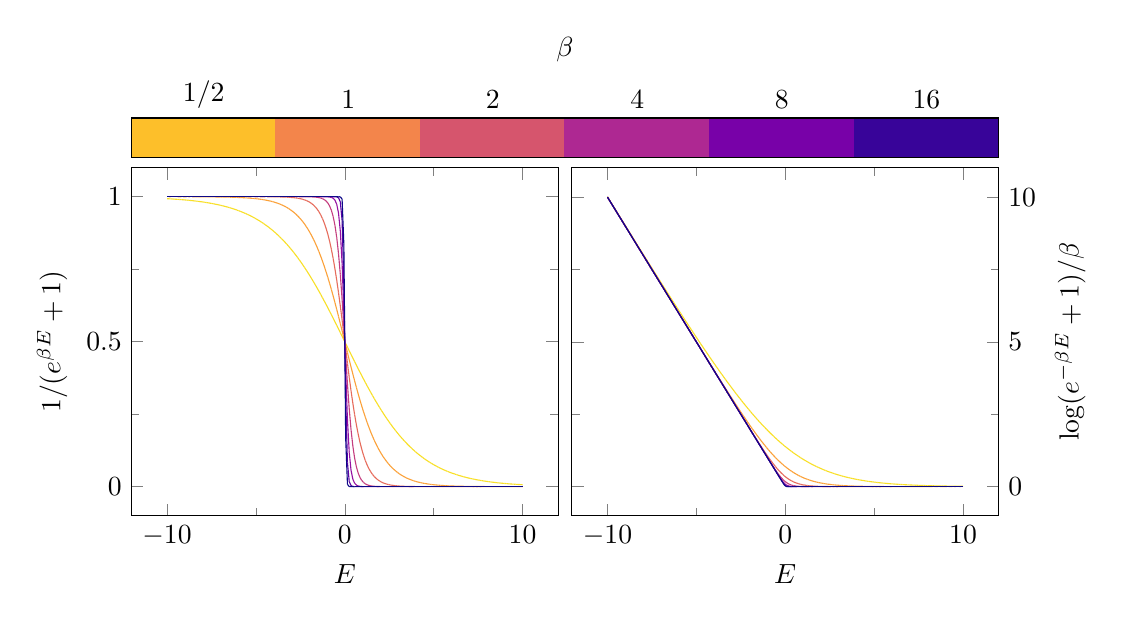
\begin{tikzpicture}
		\begin{groupplot}[group style={group size=2 by 1, horizontal sep=5pt}, height=6cm, width=7cm, /tikz/declare function={
			n(\b,\E) = 1/(exp(\b*\E)+1);
		}]
			\nextgroupplot[xlabel=$E$, ylabel=$1/(e^{\beta E}+1)$, 
				colorbar horizontal, colorbar sampled, colorbar style={xlabel=$\beta$, samples=7, xtick={-0.5, 0.5, 1.5, 2.5, 3.5, 4.5}, xticklabels={$1/2$, $1$, $2$, $4$, $8$, $16$, $32$}, grid=none, xticklabel pos=upper, tickwidth=0, at={(0.0,1.03)}, anchor=south west},
				every colorbar/.append style={width=2*\pgfkeysvalueof{/pgfplots/parent axis width}+\pgfkeysvalueof{/pgfplots/group/horizontal sep}},
				xtick distance=10, ytick distance=0.5, grid=none, minor tick num=1,
			]
			\pgfplotsinvokeforeach{0.5, 1, 2, 4, 8, 16, 32}{
				\addplot[domain=-10:+10, samples=200, mesh, point meta={log2(#1)}] {n(#1, x)};
			}

			\nextgroupplot[xlabel=$E$, ylabel=$\log (e^{-\beta E}+1)/\beta$, xtick distance=10, yticklabel pos=right, ytick distance=5, minor tick num=1, grid=none]
			\pgfplotsinvokeforeach{0.5, 1, 2, 4, 8, 16, 32}{
				\addplot[domain=-10:+10, samples=200, mesh, point meta={log2(#1)}] {ln(exp(-#1*x)+1)/#1};
			}
		\end{groupplot}
	\end{tikzpicture}
\caption{\label{fig:nstars:distribution_convergence}%
	In the zero-temperature limit $\beta E \gg 1$, the Fermi-Dirac distribution $1/(e^{\beta E}+1) \rightarrow \theta(-E)$, while $\log (e^{-\beta E} + 1) \rightarrow -\beta E \, \theta(-E)$, where $\theta(E)$ is the step function.
}
\end{figure}

In the zero-temperature limit, the Fermi-Dirac distribution can be replaced by
\begin{equation}
	n(E)       =                 \begin{cases} 1 / (e^{+\beta \abs{E}}+1) & (E>0) \\ 1 / (e^{-\beta \abs{E}}+1) & (E<0) \end{cases}
	     \quad \rightarrow \quad \begin{cases} 0 & (E>0) \\ 1 & (E<0) \end{cases}
	     \quad =                 \theta(-E) ,
\end{equation}
while the logarithm in the pressure behaves as
\begin{equation}
	\log (e^{-\beta E}+1)       =                 \begin{cases} \log (e^{-\beta \abs{E}}+1) & (E>0) \\ \log (e^{+\beta \abs{E}}+1) & (E<0) \end{cases}
	                      \quad \rightarrow \quad \begin{cases} \log 1 & (E>0) \\ \log e^{-\beta E} & (E<0) \end{cases}
	                      \quad =                 -\beta E \, \theta(-E) .
\end{equation}
This is confirmed by the plots in \cref{fig:nstars:distribution_convergence} for increasing values of $\beta$.
Thus, the zero-temperature limit effectively limits the integrals \eqref{eq:nstars:dropped_infinities} to those momenta $\vec{p}$ with $E(\vec{p}) < \mu$.
We therefore call
\begin{equation}
	\mu = E_F = E(p_F) = \sqrt{p_F^2 c^2 + m^2 c^4}
\end{equation}
the Fermi energy and the corresponding momentum $p_F$ the Fermi momentum, representing the occupied state in momentum-space with largest energy and momentum.

Now the particle density \eqref{eq:nstars:dropped_infinities_density} simply becomes
\begin{equation}
	n = 
	2 \int_0^\infty \frac{\dif p \, 4 \pi p^2}{(2 \pi \hbar)^3} \theta \left[ \mu - E(p) \right] =
	2 \int_0^{p_F} \frac{\dif p \, 4 \pi p^2}{(2 \pi \hbar)^3} = \frac{p_F^3}{3 \pi^2 \hbar^3} .
\label{eq:nstars:density_zeroT}
\end{equation}
Using integral \TODO{ref} and defining the dimensionless momentum $x = p / mc$, the energy density \eqref{eq:nstars:dropped_infinities_energy_density} is
\begin{equation}
\begin{split}
	\epsilon &=  2 \int_0^\infty \frac{\dif p \, 4 \pi p^2}{(2 \pi \hbar)^3} \, E(p) \, \theta \left[ \mu - E(p) \right] \\
	         &=  2 \int_0^{p_F} \frac{\dif p \, 4 \pi p^2}{(2 \pi \hbar)^3} \, \sqrt{p^2 c^2 + m^2 c^4} \\
	         &= \frac{m^4 c^5}{\pi^2 \hbar^3} \int_0^{x_F} \dif x \, x^2 \sqrt{1 + x^2} \\
	         &= \frac{m^4 c^5}{8 \pi^2 \hbar^3} \left[ \left( 2 x_F^3 + x_F \right) \sqrt{1 + x_F^2} - \asinh x_F \right] . \\
\end{split}
\label{eq:nstars:energy_density_zeroT}
\end{equation}
Finally, using the same integral, the pressure \eqref{eq:nstars:dropped_infinities_pressure} is
\begin{equation}
\begin{split}
	P &= \frac{2}{\beta} \int_0^\infty \frac{\dif p \, 4 \pi p^2}{(2 \pi \hbar)^3} \, \beta \left[ \mu - E(p) \right] \, \theta \left[ \mu - E(p) \right] \\
	  &= 2 \int_0^{p_F} \frac{\dif p \, 4 \pi p^2}{(2 \pi \hbar)^3} \, \left[ \sqrt{p_F^2 c^2 + m^2 c^4} - \sqrt{p^2 c^2 + m^2 c^4} \right] \\
	  &= \frac{m^4 c^5}{\pi^2 \hbar^3} \int_0^{x_F} \dif x \, x^2 \left[ \sqrt{x_F^2+1} - \sqrt{x^2+1} \right] \\
	  &= \frac{m^4 c^5}{24 \pi^2 \hbar^3} \left[ \left( 2 x_F^3 - 3 x_F \right) \sqrt{x_F^2 + 1} + 3 \asinh x_F \right] . \\
\end{split}
\label{eq:nstars:pressure_zeroT}
\end{equation}

The equation of state $\epsilon = \epsilon(P)$ follows by eliminating $x_F$ from the energy density \eqref{eq:nstars:energy_density_zeroT} and pressure \eqref{eq:nstars:pressure_zeroT}.
Due to their complicated dependence on $x_F$, we will do so in three cases of increasing difficulty.

\TODO{first present three cases, \emph{then} do calculations, to not overload the reader}

\subsection{Ultra-relativistic limit}
\label{sec:nstars:ur_limit}

First, consider the ultra-relativistic limit
\begin{equation}
	x_F \gg 1 , 
\label{eq:nstars:ur_limit}
\end{equation}
where the Fermi energy $E_F = \sqrt{p_F^2 c^2 + m^2 c^4} \taylor p_F c$ is dominated by the contribution from the Fermi momentum.
Since $\asinh x_F = \log \left[ x_F + \sqrt{x_F^2 + 1} \right] \taylor \log 2 x_F$ diverges logarithmically, we see that both the energy density \eqref{eq:nstars:energy_density_zeroT} and pressure \eqref{eq:nstars:pressure_zeroT} are dominated by their first term with $2 x_F^3 \sqrt{x_F^2 + 1} \taylor 2 x_F^4$.
In the ultra-relativistic limit, then,
\begin{equation}
	\epsilon \taylor \frac{m^4 c^5 x_F^4}{4 \pi^2 \hbar^3}
	\qquad \text{and} \qquad
	P        \taylor \frac{m^4 c^5 x_F^4}{12 \pi^2 \hbar^3},
\end{equation}
and $x_F$ is easily eliminated, yielding the very simple equation of state
\begin{equation}
	\epsilon = 3 P .
\label{eq:nstars:ur_eos}
\end{equation}

In this particular case, the TOV system \eqref{eq:tov:tovsys} can be solved analytically with the polynomial trial solution
\begin{equation}
	P(r) = A r^n .
\label{eq:nstars:ur_ansatz}
\end{equation}
Then the mass equation \eqref{eq:tov:tovsys_mass} is
\begin{equation}
	\odv{m}{r} = \frac{12 \pi A}{c^2} r^{n+2},
	\qquad \text{so} \qquad
	m(r) = \frac{12 \pi A}{(n+3) c^2} r^{n+3}
	\quad (n \neq -3).
\label{eq:nstars:ur_mass}
\end{equation}
With the equation of state \eqref{eq:nstars:ur_eos}, mass \eqref{eq:nstars:ur_mass} and trial solution \eqref{eq:nstars:ur_ansatz}, the TOV equation \eqref{eq:tov:tovsys_pressure} reads
\begin{equation}
	n A r^{n-1} =
	-\frac{48 \pi G A^2 r^{2n+1}}{(n+3) c^4} \left[ 2 + \frac{n}{3} \right] \left[ 1 - \frac{24 \pi G A r^{n+2}}{(n+3) c^4} \right]^{-1} .
\end{equation}
We can attain equality for all $r$ if we choose $n = -2$.
Then the rightmost factor no longer depends on $r$, and both sides have the same $r^{-3}$-dependence
\begin{equation}
	- 2 A r^{-3} = - \frac{64 \pi G A^2 r^{-3}}{c^4} \left[ 1 - \frac{24 \pi G A}{c^4} \right]^{-1} .
\end{equation}
Equality is established if we match the prefactors by choosing $A = c^4 / 56 \pi G$.
Then the solutions for the pressure and mass are
\begin{equation}
	P(r) = \frac{c^4}{56 \pi G} \frac{1}{r^2}
	\qquad \text{and} \qquad
	m(r) = \frac{3 c^2}{14 G} r .
\end{equation}
This is a highly unphysical result.
The pressure diverges at the center, so nothing could ever hold such a star together.
In addition, $p(r) > 0$ for all $r$, so the star has no surface and hence infinite mass $M = m(\infty) = \infty$.

\TODO{make plot of $P(r)$ and $m(r)$ for a star.}

\subsection{Non-relativistic limit}
\label{sec:nstars:nr_limit}

Next, let us consider the more difficult non-relativistic limit
\begin{equation}
	x_F \ll 1,
\label{eq:nstars:nr_limit}
\end{equation}
where the Fermi energy $E_F = \sqrt{p_F^2 c^2 + m^2 c^4} \taylor m c^2$ is dominated by the rest energy of the fermions.
Taylor expanding the energy density \eqref{eq:nstars:energy_density_zeroT} and presure \eqref{eq:nstars:pressure_zeroT} around $x_F = 0$ to lowest order, we find
\begin{equation}
	%\epsilon &\taylor \frac{m c^2 p_F^3}{3 \pi^2 \hbar^3} + \frac{p_F^5}{10 \pi^2 \hbar^3 m} = n m c^2 + \frac{p_F^5}{10 \pi^2 \hbar^3 m} \\
	%P        &\taylor \frac{p_F^5}{15 \pi^2 \hbar^3 m}
	\epsilon \taylor \frac{m c^2 p_F^3}{3 \pi^2 \hbar^3}
	\qquad \text{and} \qquad
	P        \taylor \frac{p_F^5}{15 \pi^2 \hbar^3 m} .
\end{equation}
Note that with the density \eqref{eq:nstars:density}, the energy density can be written $\epsilon = n m c^2$, so it is only due to the rest mass of the particles, as if all fermions have broken free from the Pauli exclusion principle and possess the same rest energy $m c^2$.
This is only a mathematical feature of the non-relativistic limit -- the fermions still occupy different states with different momentum, but the momenta are so small that the differences are negligible compared to the rest energy $mc^2$.
Again, it is straightforward to eliminate $x_F$ to find the equation of state, only this time there is some extra bookkeeping with all the exponents.
Carefully gathering all the prefactors under the same roof, we find
\begin{equation}
	%\epsilon = \frac{mc^2}{3\pi^2\hbar^3} \left( 15 \pi^2 \hbar^3 m P \right)^{3/5}
	\epsilon = \left( \frac{5^3 m^8 c^{10}}{3^2 \pi^4 \hbar^6} \right)^{\frac15}  P^{\frac35} .
\end{equation}
With this power dependence, it is not easy, if even possible, to solve the TOV equation analytically.
The trial solution \eqref{eq:nstars:ur_ansatz} we employed in \cref{sec:nstars:ur_limit} fails miserably, as we do not get the same fortunate cancellations of $r$.
We therefore resort to the numerical solution method described in \cref{sec:nstars:numtov}, parametrizing different stars by their center pressure $P_0$ and integrating the TOV equation until the pressure $p(R)$ vanishes, using the corresponding radius $R$ to establish the mass $M = m(R)$ of the star.
The results are shown in \cref{fig:nstars:massradius}.

\iffalse
Dimensionless equation of state
\begin{equation}
	\diml{\epsilon} = \left[ \frac{4^2 5^3}{3^4 \pi^2} \frac{m^8 c^6 r_0^6}{m_0^2 \hbar^6} \diml{P}^3 \right]^{\frac{1}{5}}
\end{equation}
\fi

\subsection{General Fermi momenta}
\label{sec:nstars:gr_limit}

How can we find the energy density
\begin{equation}
	\epsilon = \frac{m^4 c^5}{8 \pi^2 \hbar^3} \left[ \left( 2 x_F^3 + x_F \right) \sqrt{1 + x_F^2} - \asinh x_F \right]
\label{eq:nstars:gr_limit_energy_density}
\end{equation}
that corresponds to a given pressure
\begin{equation}
	P = \frac{m^4 c^5}{24 \pi^2 \hbar^3} \left[ \left( 2 x_F^3 - 3 x_F \right) \sqrt{x_F^2 + 1} + 3 \asinh x_F \right] 
\label{eq:nstars:gr_limit_pressure}
\end{equation}
for general $x_F$?
Since we are already solving the TOV equation on a computer, we can do so by numerical root finding.
At every step $r$ in the numerical integration algorithm, we know the current pressure $P = P(r)$.
Using a numerical root finding algorithm, we can find the root $x_F$ of the function
\begin{equation}
	f(x_F) = P(x_F) - P = 0,
\end{equation}
where $P(x_F)$ is the pressure \eqref{eq:nstars:gr_limit_pressure} as a function of $x_F = p_F / m c$.
Having found the root, we can simply calculate the corresponding energy density $\epsilon(x_F)$ from \cref{eq:nstars:gr_limit_energy_density}.
This whole procedure can be elegantly encapsulated into a function that implements an implicit equation of state $\epsilon = \epsilon(P)$, which in turn is straightforward to plug into our solver described in \cref{sec:nstars:numtov}.
The results are shown in \cref{fig:nstars:massradius}.

\iffalse
\begin{equation}
	\diml{P}(x_F) = \frac{m^4 c^3 r_0^3}{18 \pi m_0 \hbar^3} \left[ (2 x_F^3 - 3 x_F) \sqrt{x_F^2 + 1} + 3 \asinh x_F \right]
\end{equation}

At every integration step, we have a value of the pressure $P$.
Then find the root $x_F$ of
\begin{equation}
	P(x_F) - P = 0
\end{equation}
and then calculate
\begin{equation}
	\diml{ϵ} = \diml{ϵ}(x_F) = \diml{P}(x_F) = \frac{m^4 c^3 r_0^3}{6 \pi m_0 \hbar^3} \left[ (2 x_F^3 + x_F) \sqrt{x_F^2 + 1} - \asinh x_F \right]
\end{equation}
\fi

\tablemaximum{../code/data/nr.dat}{M}{\maxMnr}{R}{\maxRnr}
\tablemaximum{../code/data/gr.dat}{M}{\maxMgr}{R}{\maxRgr}

\begin{figure}
\centering
\begin{tikzpicture}
\begin{axis}[
	width=15cm, height=15cm,
	xlabel=$R / \si{\kilo\meter}$, ylabel=$M / \solarmass$, title={Mass-radius relation for cold free Fermi gas neutron star}, title style={yshift=2.3cm},
	xmin=0, xmax=50, xtick distance=5, minor x tick num=4,
	ymin=0, ymax=1.1, ytick distance=0.1, minor y tick num=9,
	grid=major,
	colorbar horizontal, point meta=explicit, colormap name=plasmarev, colorbar style={xlabel=$\log_{10} (P_0 / \epsilon_0)$, xtick distance=1, minor x tick num=0, at={(0.5,1.03)}, anchor=south, xticklabel pos=upper},
	%extra y ticks/.expanded={\maxMnr, \maxMgr}, extra y tick style={dashed}, % https://tex.stackexchange.com/a/333974
	%extra x ticks/.expanded={{10*\maxRnr}, {10*\maxRgr}}, extra x tick style={dashed, tick label style={yshift=-1ex}},
]
\addplot [mark=none, mesh, thick] table [x expr={10*\thisrow{R}}, y=M, meta expr={log10(\thisrow{P})}] {../code/data/nr.dat} node [pos=0.67, pin={[text=black]0:Non-relativistic limit $p_F \ll mc$}] {};
\addplot [mark=none, mesh, thick] table [x expr={10*\thisrow{R}}, y=M, meta expr={log10(\thisrow{P})}] {../code/data/gr.dat} node [pos=0.61, pin={[text=black]-100:Arbitrary $p_F$}] {};
\node [circle, fill, inner sep=1pt, label={90:$(\pgfmathprintnumber\maxRnr, \pgfmathprintnumber\maxMnr)$}] at ({10*\maxRnr}, \maxMnr) {};
\node [circle, fill, inner sep=1pt, label={90:$(\pgfmathprintnumber\maxRgr, \pgfmathprintnumber\maxMgr)$}] at ({10*\maxRgr}, \maxMgr) {};

%\edef\doplot{\noexpand\addplot [domain=-10:10, dashed, update limits=false] {\maxM};} % see https://tex.stackexchange.com/a/73916, https://tex.stackexchange.com/a/519
%\doplot

\end{axis}
\end{tikzpicture}

\caption{\label{fig:nstars:massradius}%
Mass-radius relation for cold neutron stars parametrized by their central pressures $P_0$, obtained by numerically integrating the TOV equation from the central pressure $P_0$ until it vanishes at the surface $R$.
The numerical integration is carried out using an explicit equation of state in the non-relativistic limit with Fermi momenta $p_F \ll m c$, and using a root-finding algorithm to calculate an implicit equation of state for general $p_F$.
Stars are parametrized by central pressures $\SI{1e-6}{} \epsilon_0 \le P_0 \le \SI{1e7}{} \epsilon_0$, where $\epsilon_0 = \solarmass c^2 / (4 \pi R_0^3 / 3) = \SI{4.27e34}{\pascal}$, $R_0 = \SI{10}{\kilo\meter}$, $\solarmass$ is the mass of the sun and $c$ is the speed of light.
}

\end{figure}

\begin{figure}
\centering
\begin{tikzpicture}
\begin{groupplot}[
	group style={group size=1 by 2, vertical sep=10pt},
	width=14cm, height=9cm,
	ylabel=$M / \solarmass$, 
	grid=major,
	%point meta=explicit, point meta min=-1.5, point meta max=+1.5,
	colormap={signnegpos}{samples of colormap=(4 of stability)}, colormap access=const, 
	point meta=explicit, point meta min=0, point meta max=4,
	every axis title/.style={at={(0.97,0.95)}, text width=3cm, anchor=north east, draw=black, fill=white},
]
\nextgroupplot[
	title={\subcaption{\label{fig:nstars:stability_computed}Computed}},
	colorbar horizontal, colorbar sampled, colorbar style={xlabel={Number of unstable modes with $\omega_n^2 < 0$}, xtick={0.5, 1.5, 2.5, 3.5}, xticklabels={$0$, $1$, $2$, $3$}, at={(0.5,1.05)}, anchor=south, xticklabel pos=upper, tickwidth=0},
	xticklabels=\empty,
]
\addplot [mark=none, mesh, thick] table [x expr={10*\thisrow{R}}, y=M, meta=nu] {../code/data/gr2.dat};

\nextgroupplot[
	title={\subcaption{\label{fig:nstars:stability_exact}Exact}},
	xlabel=$R / \si{\kilo\meter}$,
]
\addplot [mark=none, mesh, thick] table [x expr={10*\thisrow{R}}, y=M, meta expr={greater(\thisrow{P},0.8) + greater(\thisrow{P},600) + greater(\thisrow{P},19000)}] {../code/data/gr2.dat};
\end{groupplot}
\end{tikzpicture}

\caption{\label{fig:nstars:stability}%
Stability analysis of the neutron stars with arbitrary Fermi momenta in \cref{fig:nstars:massradius}.
The sign of the squared eigenfreuqency $\omega_0^2$ of the lowest normal vibration mode determines whether a star is stable and oscillates like $e^{i \omega_0 t}$, or if it is unstable and grows or decays like $e^{\pm \abs{\omega_0} t}$.
\subref{fig:nstars:stability_computed} Squared eigenfrequencies computed numerically by solving the Sturm-Liouville eigenvalue equation with the shooting method.
\subref{fig:nstars:stability_exact} Stability determined exactly by the rule that a star transitions from stable to unstable as the central pressure increases beyond the one corresponding to the maximum mass.
}

\end{figure}

\section{Stability analysis}

The mass-radius curves in \cref{fig:nstars:massradius} display some interesting behavior.
In particular, the curves spiral for central pressures greater than that corresponding to the maximum mass.
Since we have used statistical physics to obtain an equation of state, all stars on the mass-radius curve are in \emph{equilibrium}.
\TODO{is the assumption of equilibrium instead/also baked into using perfect fluid energy momentum \eqref{eq:tov:energy_momentum_perfect_fluid}? and $U = (U^0, \vec{0})$?}
However, just like a pendulum can be in stable or unstable equilibria, the equilibrium of a star can be either stable or unstable with respect to small perturbations.
Let us investigate the stability of the sequence of stars on the curve in \cref{fig:nstars:massradius}.

\TODO{figure with analogy between unstable pendulum and unstable star?}

\subsection{Necessary conditions for stability}

We will start simple by presenting a few necessary conditions for stability.
However, neither of the conditions are \emph{sufficient} or a star to be stable, so we can only use them to identify unstable stars.

However exotic life inside a star may be, it cannot break causality. 
In particular, the speed of sound $v = \sqrt{\odv{P}/{\rho}} = c \sqrt{\odv{P}/{\epsilon}}$ should not exceed the speed of light $c$.
The equation of state $\epsilon = \epsilon(P)$ must therefore satisfy
\TODO{ref?}
\begin{equation}
	\odv{P}{\epsilon} < 1 .
\end{equation}
How does the equation of state for a free Fermi gas hold up in this regard?
Recall that the equation of state for general Fermi momenta $p_F$ followed by eliminating $x_F$ from the energy density \eqref{eq:nstars:energy_density_zeroT} to express it in terms of the pressure \eqref{eq:nstars:pressure_zeroT}.
It is straightforward to calculate the derivatives
\begin{equation}
	\odv{P}{x_F} = \frac{m^4 c^5}{3 \pi^2 \hbar^3} \frac{x_F^4}{\sqrt{x_F^2 + 1}}
	\quad \text{and} \quad
	\odv{\epsilon}{x_F} = \frac{m^4 c^5}{\pi^2 \hbar^3} x_F^2 \, \sqrt{x_F^2 + 1} .
\end{equation}
Then we can apply the chain rule and the rule of inverse derivatives to obtain
\begin{equation}
	\odv{P}{\epsilon} = 
	\odv{P}{x_F} \odv{x_F}{\epsilon} =
	\frac{\odv{P}/{x_F}}{\odv{\epsilon}/{x_F}} =
	\frac13 \, \frac{1}{1+1/x_F^2}.
\end{equation}
We see that $\odv{P}/{\epsilon} < 1$ for all $x_F$ and approaches $1/3$ in the ultra-relativistic limit $x_F \rightarrow \infty$, as we should expect from the corresponding equation of state \eqref{eq:nstars:ur_eos}.
Hence, all the stars in \cref{fig:nstars:massradius} satisfy this condition and it does not rule out any stars.

\usetikzlibrary{arrows.meta}
\usetikzlibrary{shapes.symbols}
\begin{figure}
\begin{tikzpicture}
\newcommand\drawstarforcebalance[8]{
	\draw [very thick, inner color=yellow!#6!gray, outer color=red!#6!gray] (#1,#2) circle [radius=#3];
	\draw [thick] [-{Latex[width=#7mm,length=#7mm]}] ({#1-0.1},{#2+0.1}) -- ({#1-0.1+#4*cos(45)},{#2+0.1+#4*sin(45)});
	\draw [thick] [{Latex[width=#8mm,length=#8mm]}-] ({#1+0.1},{#2-0.1}) -- ({#1+0.1+#5*cos(45)},{#2-0.1+#5*sin(45)});
}
\drawstarforcebalance{0.0}{0.0}{1.0}{0.9}{0.9}{0}{4}{4};
\drawstarforcebalance{3.0}{0.0}{1.5}{1.4}{0.7}{33}{5}{3};
\drawstarforcebalance{7.0}{0.0}{2.0}{1.9}{0.5}{66}{6}{2};
\node[starburst, fill=yellow, draw=red, line width=2pt, anchor=west, minimum size=5cm] at (10,0) {\huge\textbf{BOOM}};
\end{tikzpicture}
\caption{\label{fig:nstars:star_explosion}%
A slight decrease $\dif \epsilon < 0$ in energy density weakens the gravitational force pulling a star in.
If the equation of state $\epsilon = \epsilon(P)$ in a star satisfies $\odv{P}/{\epsilon} < 0$, such a change in energy density would cause an increase $\dif P > 0$ in the pressure pushing the star out.
The greater pressure then causes the star to expand, which in turn causes another decrease in energy density.
Repeated application of the same argument shows that the star continues to expand while the pressure grows indefinitely, so the star ultimately explodes.
}
\end{figure}

From the expression $v = c \sqrt{\odv{P}/{\epsilon}}$ of the speed of sound, it also sounds reasonable to require that
\begin{equation}
	\odv{P}{\epsilon} > 0
\label{eq:nstars:stability_pressure_energy_density}
\end{equation}
for it to be a real quantity.
Violation of this condition would in fact have dramatic consequences.
First, note that an increase in energy density $\dif \epsilon > 0$ always increase the gravitational force attempting to pull the star in.
If such an increase implied a \emph{decrease} $\dif P < 0$ in the pressure that pushes the star out, then the gravitational force would automatically ``win'', causing the star to contract, and hence the energy density to increase further.
Repeating the argument, we understand that the star collapses.
This process is illustrated in \cref{fig:nstars:stability_mass_pressure}.
Likewise, if a decrease $\dif \epsilon < 0$ caused an increase $\dif P > 0$, the same argument shows that the pressure wins and the star explodes.
However, if the two always change by the same sign, then the two forces will at the very least counteract each other instead of being driven apart.
In this case the star \emph{can} be stable, but the balance between the forces would have to be investigated in detail to conclude if it \emph{is}.
This criterion does not let us rule out any of our stars, either, but it will be useful to assume \TODO{ref} in the following.

\begin{figure}
\centering
\begin{tikzpicture}
\begin{axis}[axis x line=bottom, axis y line=left, xlabel=$P_0$, ylabel=$M$, xtick=\empty, ytick=\empty]
	\addplot[domain=-1:+1, black] {-x^2};

	\node [draw=black, circle, fill, inner sep=1pt, label=left:$E_1$] at (axis cs:-0.7,-0.49) {};
	\node [draw=black, circle, fill, inner sep=1pt, label=left:$E_2$] at (axis cs:-0.5,-0.25) {};
	\node [draw=black, circle, fill, inner sep=1pt, label=right:$C$ ] at (axis cs:-0.5,-0.49) {};

	\node [draw=black, circle, fill, inner sep=1pt, label=left:$E_2$] at (axis cs:+0.7,-0.49) {};
	\node [draw=black, circle, fill, inner sep=1pt, label=left:$E_1$] at (axis cs:+0.5,-0.25) {};
	\node [draw=black, circle, fill, inner sep=1pt, label=right:$C$ ] at (axis cs:+0.7,-0.25) {};
\end{axis}
\end{tikzpicture}
\caption{\label{fig:nstars:stability_mass_pressure}}
\end{figure}

A third necessary condition is
\begin{equation}
	\odv{M(P_0)}{P_0} > 0
\label{eq:nstars:stability_mass_pressure}
\end{equation}
for stars parametrized by their central pressure $P_0$.

Consider a star $E_1$ in equilibrium on the increasing part of the curve in \cref{fig:nstars:stability_mass_pressure}, where condition \eqref{eq:nstars:stability_mass_pressure} is satisfied.
Now compress this star to the non-equilibrium star $C$ with the same mass, and let $E_2$ be the star in equilibrium with the same central pressure as $C$.
Then $C$ has less mass than $E_2$, and hence weaker gravitational forces than $E_2$, but the same central pressure as $P_2$.
As a result, the star will expand and decrease its central density and pressure, causing it to return towards the equilibrium star $E_1$.

Let us we repeat the argument on the decreasing part of the curve, where condition \eqref{eq:nstars:stability_mass_pressure} does not hold.
After the compression from $E_1$ to $C$, we see that $C$ has more mass and hence stronger gravitational forces than $E_2$, but again the same central pressure.
The star therefore contracts, and repeating the argument causes it to collapse completely.

The criterion \eqref{eq:nstars:stability_mass_pressure} shows that the stars located between the maximum mass and the bottom of the spiral in \cref{fig:nstars:massradius} are unstable!

\subsection{General analysis}

\TODO{where to put this?}
Then he expanded the field equations to first order in the deviations $\delta f$ and simplified them by subtracting the equilibrium equations \eqref{eq:nstars:field_equations_equilibrium}.
Chandrasekhar's original paper \cite{ref:chandrasekhar_stability} is very compact and does not include many details of this calculation.
A more verbose outline can be found in \cite[§ 26.4d]{ref:mtw}, which we will follow here.
\TODO{but we dont do all details}


The arguments presented above were necessary, but not sufficient for stellar stability.
Let us analyze the stability of the stars in a more rigorous way by finding a mathematical definition of stability.

In \cref{sec:einstein_to_tov}, we showed that the Einstein field equations \eqref{eq:einstein} reduced to
\TODO{start with metric}
\begin{subequations}%
\begin{align}%
	\frac{1}{r^2} e^{-2 \beta_0} \left( 2 r \beta_0' - 1 + e^{2 \beta_0} \right)  &= \frac{8 \pi G}{c^4} \epsilon_0   && \left( G_{00} = \frac{8 \pi G}{c^4} T_{00} \right) , \label{eq:nstars:field_equations_equilibrium_00} \\
	\frac{1}{r^2} e^{-2 \beta_0} \left( 2 r \alpha_0' + 1 - e^{2 \beta_0} \right) &= \frac{8 \pi G}{c^4} P_0          && \left( G_{11} = \frac{8 \pi G}{c^4} T_{11} \right) , \label{eq:nstars:field_equations_equilibrium_11} \\
	\alpha_0'                                                                     &= \frac{-1}{\epsilon_0 + P_0} P_0' && \left( \nabla_\mu T\indices{^\mu_1} = 0 \right)    . \label{eq:nstars:field_equations_equilibrium_T}
	%e^{-2 \beta_0} \left( \alpha_0'' + (\alpha_0')^2 - \alpha_0' \beta_0' + \frac{1}{r} (\alpha_0' - \beta_0') \right) &= \frac{8 \pi G}{c^4} P_0,
\end{align}%
\label{eq:nstars:field_equations_equilibrium}%
\end{subequations}%
for a perfect fluid with energy-momentum
\begin{equation}
	T_{\mu \nu} = \frac{1}{c^2} U_\mu U_\nu (\epsilon_0 + P_0) - g_{\mu \nu} P_0
	\quad \text{where} \quad
	P_0 = P_0(r), \epsilon_0 = \epsilon_0(r) ,
\label{eq:nstars:energy_momentum}
\end{equation}
in \emph{equilibrium} with four-velocity
\begin{equation}
	U^\mu = (U^0, 0,0,0) ,
\label{eq:nstars:velocity_equilibrium}
\end{equation}
in the spherically symmetric metric
\begin{equation}
	\dif s^2 = e^{2 \alpha_0(r)} \dif t^2 - e^{2 \beta_0(r)} \dif r^2 - r^2 \left( \dif \theta^2 + \sin^2 \theta \dif \phi^2 \right) .
\end{equation}

Now we suppose that the fluid is \emph{no longer in equilibrium}, \TODO{better word?} but rather has the four-velocity
\begin{equation}
	U^\mu = (U^0, U^1, 0, 0)
	\quad
	\text{with a non-zero radial component $U^1$.}
\label{eq:nstars:velocity_unstable}
\end{equation}
By the spherical symmetry, we still assume there is no angular velocity component.
The metric should still be spherically symmetric, but $\alpha_0(r) \rightarrow \alpha(r,t)$ and $\beta_0(r) \rightarrow \beta(r,t)$ are promoted to time-dependent functions, and therefore so are the pressure $P_0(r) \rightarrow P(r,t)$ and energy density $\epsilon_0(r) \rightarrow \epsilon(r,t)$.
We therefore have the new metric
\begin{equation}
	\dif s^2 = e^{2 \alpha(t, r)} \dif t^2 - e^{2 \beta(t, r)} \dif r^2 - r^2 \left( \dif \theta^2 + \sin^2 \theta \dif \phi^2 \right) .
\label{eq:nstars:metric_unstable}
\end{equation}
To make calculations manageable, we assume that the fluid is only slightly \emph{perturbed} from equilibrium.
Following \cite{ref:chandrasekhar_stability}, our strategy will be to employ perturbation theory by writing the new functions as the small perturbations 
\begin{equation}
\begin{aligned}
	\alpha   (r, t) &= \alpha_0  (r) + \delta \alpha  (r, t), & \qquad \qquad
	\beta    (r, t) &= \beta_0   (r) + \delta \beta   (r, t), \\
	P        (r, t) &= P_0       (r) + \delta P       (r, t), & \qquad \qquad
	\epsilon (r, t) &= \epsilon_0(r) + \delta \epsilon(r, t), \\
\end{aligned}
\label{eq:nstars:perturbation_expansion}
\end{equation}
around equilibrium, and calculating the perturbations to first order.

The fundamental quantity that we want to determine is the displacement $\xi(t, r)$ of fluid elements from the unperturbed to the perturbed system.
Evolution of this quantity should give us insight into how the stellar material responds to perturbations.
Like $\delta \alpha$, $\delta \beta$, $\delta P$ and $\delta \epsilon$, we assume $\xi$ be a small quantity, and we will calculate to first order in all these five quantites.
Let us define $\xi(t, r)$ it so that if we attach a tracker to some fixed fluid element in the star, then
\TODO{I should not mention $\xi$ before it is defined}
\begin{equation}
\begin{split}
	\text{      in the unperturbed star, } & \text{the fluid element is at $\big(ct,r,\theta,\phi\big)$,} \\
	\text{while in the   perturbed star, } & \text{the fluid element is at $\big(ct,r+\xi(r,t),\theta,\phi\big)$.} \\
\end{split}
\end{equation}
What is the relation between the fluid element displacement $\xi(r,t)$ and the fluid's four-velocity?
By our definition, $\pdv{\xi}/{t} = \odv{r}/{t}$, where the latter derivative is the derivative of the fluid element's radial coordinate taken \emph{along its world line} -- or \emph{stream line} -- $x(\tau)$.
The chain rule then gives
\begin{equation}
	\dot\xi = \pdv{\xi}{t} = \odv{r}{t} = \frac{\odv{r}/{\tau}}{\odv{t}/{\tau}} = c \, \frac{U^1}{U^0} .
\end{equation}
We can determine $U^0$ and $U^1$ by combining this equation the normalization condition $U_\mu U^\mu = e^{2 \alpha} \left( U^0 \right)^2 - e^{2 \beta} \left( U^1 \right)^2 = c^2$.
To first order in $\xi$ and $\delta \alpha$, we find the components
\begin{equation}
	U^0%=       c \, \frac{U^1}{\dot\xi}
	    =       c \, \frac{e^{-\alpha}}{\sqrt{1 - \left( \frac{e^\beta \dot\xi}{c e^\alpha} \right)^2 }}
	    \taylor c \, e^{-\alpha_0} \, (1 - \delta \alpha)
	\qquad \text{and} \qquad
	U^1 =        \frac{e^{-\alpha}}{\sqrt{1 - \left( \frac{e^\beta \dot\xi}{c e^\alpha} \right)^2 }} \, \dot\xi
	    \taylor  e^{-\alpha_0} \dot\xi .
\end{equation}

In the perturbed system, the field equations \eqref{eq:nstars:field_equations_equilibrium} also change and must be rederived from the Einstein equations \eqref{eq:einstein} in the new metric \eqref{eq:nstars:metric_unstable} subject to the energy-momentum \eqref{eq:nstars:energy_momentum} with the non-equilibrium velocity \eqref{eq:nstars:velocity_unstable}.
As always, the field equations follow from the machinery of \cref{eq:def_christoffel,eq:def_riemann_tensor,eq:def_ricci_tensor,eq:def_ricci_scalar}.
This time, we calculate the field equations to first order in the small quantities and subtract the equilibrium equations \eqref{eq:nstars:field_equations_equilibrium} to simplify them.
A tedious, but in principle straightforward calculation (although in practice perhaps not), reveals that to first order in the perturbations, two of the new field equations are
\begin{subequations}
\begin{align}
	%\delta \beta   &= - \frac{4 \pi G}{c^4} (\epsilon_0 + P_0) r e^{2 \beta_0} \xi                                                                                                && \left( G_{01} = \frac{8 \pi G}{c^4} T_{01} \right) , \\
	%\delta \alpha' &= \frac{r}{2 e^{-2 \beta_0}} \left[ \frac{8 \pi G}{c^4} \delta P + 2 e^{-2 \beta_0} \left( \frac{2}{r} \alpha_0' + \frac{1}{r^2} \right) \delta \beta \right] && \left( G_{11} = \frac{8 \pi G}{c^4} T_{11} \right) .
	%%\delta \alpha' &= 4 \pi \left\{ -\gamma P_0 \frac{e^{2 \beta_0}}{r} (r^2 e^{-\alpha_0} \xi)' + \left[ P_0' r - (\epsilon_0 + P_0) e^{2 \beta_0} \xi \right] \right\}
	%
	\frac{2}{r} e^{-(\beta_0 + \alpha_0)} \dot{\delta\beta}                                                                     &= - \frac{8 \pi G}{c^4} (\epsilon_0 + P_0) e^{\beta_0 - \alpha_0} \dot\xi                         && \left( G_{01} = \frac{8 \pi G}{c^4} T_{01} \right) , \label{eq:nstars:field_equations_unstable_01} \\
	\frac{2}{r} e^{-2\beta_0} \delta\alpha' - 2 e^{-2 \beta_0} \left( \frac{2}{r} \alpha_0' + \frac{1}{r^2} \right) \delta\beta &= \frac{8 \pi G}{c^4} \delta P                                                                    && \left( G_{11} = \frac{8 \pi G}{c^4} T_{11} \right) . \label{eq:nstars:field_equations_unstable_11}
\end{align}
\TODO{integrate first with time!}
\Cref{eq:nstars:field_equations_unstable_01,eq:nstars:field_equations_unstable_11} are analogous to \cref{eq:nstars:field_equations_equilibrium_00,eq:nstars:field_equations_equilibrium_11}.
What is the third equation corresponding to \cref{eq:nstars:field_equations_equilibrium_T}, which we found from conservation of energy-momentum $\nabla_\mu T^{\mu \nu} = 0$?
In \cref{chap:relfluid}, we study relativistic fluid mechanics and start from $\nabla_\mu T^{\mu \nu} = 0$ to derive the relativistic generalization of the Euler equation,
\begin{equation*}
	  \frac{1}{c^2} \Big( \epsilon + P \Big) U^\mu \nabla_\mu U^\alpha = \nabla^\alpha P - \frac{1}{c^2} U^\alpha U^\mu \nabla_\nu P
	  \qquad \left( \nabla_\mu T^{\mu \nu} = 0 \right) .
\end{equation*}
By inserting the new four-velocity \eqref{eq:nstars:velocity_unstable} and the expansions \eqref{eq:nstars:perturbation_expansion} into the relativistic Euler equation and performing calculations in the new metric \eqref{eq:nstars:metric_unstable} to first order, one finds
\TODO{ref program?}
\begin{equation}
	\left( \epsilon_0 + P_0 \right) e^{2 \beta_0 - 2 \alpha_0} \ddot \xi = -c^2 \left[ \delta P' - \left( \delta \epsilon + \delta P \right) \alpha_0' - \left( \epsilon_0 + P_0 \right) \delta \alpha' \right] .
\label{eq:nstars:field_equations_unstable_T}
\end{equation}
\label{eq:nstars:field_equations_unstable}%
\end{subequations}
The system \eqref{eq:nstars:field_equations_unstable} consists of \emph{three} equations for the \emph{five} unknowns $\xi$, $\delta P$, $\delta \epsilon$, $\delta \alpha$ and $\delta \beta$.
We will complete the set by finding two additional equations from our study of relativistic fluid mechanics in \cref{chap:relfluid}.

To make use of the results of \cref{chap:relfluid} in our context, we must first learn to distinguish between \emph{Eularian} and \emph{Lagrangian} changes in fluids.
The quantities
\begin{subequations}
\begin{equation}
	\delta f(r, t) = f(r, t) - f_0(r)
\label{eq:nstars:change_eularian}
\end{equation}
that we defined in \cref{eq:nstars:perturbation_expansion} are \textbf{Eularian changes} in the quantities $f$, measured by an observer who is sitting duck at some fixed position $x^\mu = (ct, r, \theta, \phi)$.
In contrast, we define the \textbf{Lagrangian changes}
\begin{equation}
	\Delta f(r,t) = f(r+\xi(r,t), t) - f_0(r)
\label{eq:nstars:change_lagrangian}
\end{equation}
\end{subequations}
as the changes in the same quantities, but measured by an observer who is moving \emph{with} the fluid element as it flows from $r$ to $r + \xi(r,t)$.
One can always be converted to the other through the Taylor expansion
\begin{equation}
\begin{split}
	\Delta f(r,t) &\taylor f(r,t) + \xi(r,t) \, f'(r,t) - f_0(r) \\
	              &= \delta f(r,t) + \xi(r,t) \, f'(r,t) .
\end{split}
\label{eq:nstars:delta_taylor_expansion}
\end{equation}
To summarize, $\delta$ measures changes at a fixed position of different fluid elements, while $\Delta$ measures changes of fixed fluid elements at different positions.
The first stems from perturbation theory, and the second is natural to use in fluid mechanics.

In our study of relativistic fluid mechanics in \cref{chap:relfluid}, we require that the number of baryons in a fluid element must be conserved in flow.
By eliminating the baryon number density with \cref{eq:relfluid:baryon_number_rate_change}, the equation of energy conservation \eqref{eq:relfluid:energy_conservation_rewritten} is equivalent to
\TODO{say that we eliminate baryon number density}
\begin{equation}
	\odv{\epsilon}{\tau} = -(\epsilon+P) \nabla_\mu U^\mu 
\label{eq:nstars:energy_conservation}
\end{equation}
First, note that because the equilibrium energy density $\epsilon_0(r)$ is independent of time, $\odv{\epsilon}/{\tau} = \odv{\Delta \epsilon}/{\tau}$.
At first sight, it may sound more straightforward to write $\odv{\delta \epsilon}/{\tau}$ instead of $\odv{\Delta \epsilon}/{\tau}$.
However, since the derivative $\odv{}/{\tau}$ is along the stream line of the fluid element, the Lagrangian changes are more accurate than the Eularian changes to first order in perturbation theory.
To first order in the small quantities, only the time component contributes when applying the chain rule to the left side
\begin{equation}
	\odv{\epsilon}{\tau} =
	\odv{\Delta \epsilon}{\tau} =
	U^\mu \nabla_\mu \Delta \epsilon \taylor
	U^0 \pdv{\Delta \epsilon}{t} = U^0 \dot{\Delta \epsilon} =
	e^{-\alpha_0} \dot{\Delta \epsilon} .
\end{equation}
On the right side, we can calculate the quantity $\nabla_\mu U^\mu$ with the identity
\begin{equation}
\begin{split}
	\nabla_\mu U^\mu &= \frac{1}{\sqrt{-\det{g}}} \partial_\mu \left( \sqrt{-g} \, U^\mu \right) \\
	                 &= e^{-\alpha_0} \left[ \dot{\delta\beta} + \frac{e^{-\beta_0}}{r^2} \left( e^{\beta_0} r^2 \dot\xi \right)' \right] .
\end{split}
\end{equation}
To first order in the small quantities, \cref{eq:nstars:energy_conservation} then says
\begin{equation}
	\dot{\Delta \epsilon} = - \left( \epsilon_0 + P_0 \right) \left[ \dot{\delta\beta} + \frac{e^{-\beta_0}}{r^2} \left( e^{\beta_0} r^2 \dot\xi \right)' \right] .
\end{equation}
Again, integrate with respect to time to get rid of the dots and set the integration constant to zero, so $\Delta \epsilon = 0$ when $\delta \beta = 0$ and $\xi = 0$.
We then find our fourth main equation
\begin{equation}
	\Delta \epsilon = - \left( \epsilon_0 + P_0 \right) \left[ \delta\beta + \frac{e^{-\beta_0}}{r^2} \left( e^{\beta_0} r^2 \xi \right)' \right] .
\label{eq:nstars:Delta_epsilon}
\end{equation}

The last result of \cref{chap:relfluid} that we make use of is adiabadicity of the flow.
In \cref{sec:relfluid:adiabadicity}, we show that the flow of a perfect fluid is adiabatic with the \textbf{adiabatic index}
\begin{equation}
	\gamma = \frac{\epsilon+P}{P} \odv{P}{\epsilon} .
\label{eq:nstars:adiabatic_index0}
\end{equation}
The above expression can be calculated entirely from the fluid's equation of state $\epsilon = \epsilon(P)$, although in its current form, it is the perturbed quantities that enter, so for now it must be treated as an unknown quantity.
However, by interpreting the derivative as the ratio of Lagrangian changes, the adiabatic index can be rewritten in the visually similar, but fundamentally distinct form
\begin{equation}
	\gamma = 
	\frac{\epsilon+P}{P} \frac{\Delta P}{\Delta \epsilon} ,
	\quad \text{or} \quad
	\Delta P = \frac{P}{\epsilon + P} \, \gamma \, \Delta \epsilon .
\label{eq:nstars:adiabatic_index}
\end{equation}
\TODO{what about $P$ vs $P_0$ here?}
The latter is a relation between two first order quantities, and so for the purpose of perturbation theory, \emph{the only relevant part of $\gamma$ is the zeroth order part}
\begin{equation}
	\gamma_0 = \frac{\epsilon_0+P_0}{P_0} \frac{\Delta P_0}{\Delta \epsilon_0} .
\end{equation}
This gives us our fifth and final equation
\begin{equation}
	\Delta P = \frac{P_0}{\epsilon_0 + P_0} \, \gamma_0 \, \Delta \epsilon .
\label{eq:nstars:Delta_P}
\end{equation}

We have made quite a big mess by now, but we finally have all the information we need, and it remains only to clean up after ourselves.
Together, \cref{eq:nstars:field_equations_unstable_01,eq:nstars:field_equations_unstable_11,eq:nstars:field_equations_unstable_T,eq:nstars:Delta_epsilon,eq:nstars:Delta_P} constitute the system of five equations
\begin{subequations}
\begin{align}
	\frac{2}{r} e^{-(\beta_0 + \alpha_0)} \delta\beta                                                                           &= - \frac{8 \pi G}{c^4} (\epsilon_0 + P_0) e^{\beta_0 - \alpha_0} \xi \\
	\frac{2}{r} e^{-2\beta_0} \delta\alpha' - 2 e^{-2 \beta_0} \left( \frac{2}{r} \alpha_0' + \frac{1}{r^2} \right) \delta\beta &= \frac{8 \pi G}{c^4} \delta P                                  \\
	\left( \epsilon_0 + P_0 \right) e^{2 \beta_0 - 2 \alpha_0} \ddot \xi                                                        &= -c^2 \left[ \delta P' - \left( \delta \epsilon + \delta P \right) \alpha_0' - \left( \epsilon_0 + P_0 \right) \delta \alpha' \right] \\
	\Delta \epsilon                                                                                                             &= - \left( \epsilon_0 + P_0 \right) \left[ \delta\beta + \frac{e^{-\beta_0}}{r^2} \left( e^{\beta_0} r^2 \xi \right)' \right]  \\
	\Delta P &= \frac{P_0}{\epsilon_0 + P_0} \, \gamma_0 \, \Delta \epsilon
\end{align}%
\label{eq:nstars:perturbation_system}%
\end{subequations}%
for the five unknowns $\xi$, $\delta \alpha$, $\delta \beta$, $\delta P$ and $\delta \epsilon$.
Remember that any occurence of $\Delta P$ and $\Delta \epsilon$ can be traded for $\delta P$ and $\delta \epsilon$ by the Taylor expansion \eqref{eq:nstars:delta_taylor_expansion}.
Except for the independent variables $r$ and $t$, the only other quantities are the equilibrium values $\alpha_0$, $\beta_0$, $P_0$ and $\epsilon_0$ and derivatives thereof.
Solving the Tolman-Oppenheimer-Volkoff equations \eqref{eq:tov:tovsys} yield $P_0$, $m_0$ and $\alpha_0$, from which one can calculate $\epsilon_0$ by the equation of state \eqref{eq:tov:tovsys_eos} and $\beta_0$ from definition \eqref{eq:einstein_to_tov:def_m}.

As we remarked earlier, it is $\xi$ we want to calculate, so let us reduce the system \eqref{eq:nstars:perturbation_system} to a differential equation involving $\xi(t,r)$ as the only dependent variable.
Along the way, it is convenient to define
\begin{equation}
	\zeta(t,r) = r^2 e^{\beta_0(r)} \xi(t,r),
\end{equation}
because the only spatial derivative of $\xi$ appears in the combination $\left( e^{\beta_0} r^2 \xi \right)$.
Never forget that we are doing perturbation theory, so any product of two small quantities can be neglected, and we can simplify expressions using any equilibrium equation from above.
Again, the work before us is easy in principle and hard in practice.
In the end, one finds that $\zeta$ obeys the differential equation
\begin{equation}
	W(r) \ddot{\zeta}(r,t) = (\Pi(r) \zeta'(r))' + Q(r) \zeta(r) ,
\label{eq:nstars:diffeq_zeta}
\end{equation}
where the coefficient functions are
\TODO{use big/small $u$/$U$ in ST-eq/4-vel}
\TODO{check units}
\begin{subequations}
\begin{align}
	\Pi &= \frac{1}{r^2} e^{\beta_0 + 3 \alpha_0} \gamma P_0 , \\
	Q   &= -\frac{4}{r^3} e^{\beta_0 + 3 \alpha_0} P_0' - \frac{8 \pi}{r^2} e^{3 \beta_0 + 3 \alpha_0} P (\epsilon_0 + P_0) + \frac{e^{\beta_0 + 3 \alpha_0}}{r^2(\epsilon_0 + P_0)} (P_0')^2 , \\
	W   &= \frac{1}{r^2} e^{3 \beta_0 + \alpha_0} (\epsilon_0 + P_0) .
\end{align}
\label{eq:nstars:sturm_liouville_coefficients}
\end{subequations}

\TODO{incorporate how to find $\alpha_0$ into TOV chapter and/or code appendix}
In addition, $\alpha$ can be obtained by integrating its derivative \eqref{eq:einstein_to_tov:dadr1} or \eqref{eq:einstein_to_tov:dadr2}, too.
Since it is only the derivative of $\alpha$ that enters the TOV equation, we can start its integration subject to a convenient boundary condition such as $\alpha(0) = 0$.
Then, at the end, we shift $\alpha(r) \rightarrow \alpha(r) - \alpha(R) + \frac12 \log (1 - 2 G M / R)$ to match it to the Schwarzschild solution.

We can find a general solution of this equation using separation of variables.
Let us write
\begin{equation}
	\zeta(t,r) = T(t) \, U(r) .
\end{equation}
Substitution into the differential equation \eqref{eq:nstars:diffeq_zeta} shows that
\begin{equation}
	\frac{\ddot{T}}{T} = \frac{\left( \Pi \, U' \right)' + Q \, U}{W} = -\omega^2
\end{equation}
must be a constant $-\omega^2$, so we find that $T(t) = e^{i \omega t}$ and that $U(r)$ and $\omega^2$ must solve
\begin{equation}
	\odv*{ \left[ \Pi(r) \odv{U(r)}{r} \right] }{r} + \left[ Q(r) + \omega^2 W(r) \right] U(r) = 0 .
\label{eq:nstars:sturm_liouville}
\end{equation}

What are the boundary equations for $U(r)$?
At the center $r = 0$, spherical symmetry implies that there can be no flow, so the physical boundary condition there is
\begin{equation}
	\xi(t, 0) = 0.
\label{eq:nstars:boundary_condition_center_physical}
\end{equation}
If there was flow at the center, it would necessarily be uniform in all directions, so an inward flow would drain all of the star's material into a sink at the center, while an outward flow would expel the material and create an ``eye of the storm'' in the middle.
The translation of this condition for the displacement \eqref{eq:nstars:displacement_general_solution} to vanish is
\TODO{why not $r^4$, $r^5$, etc? do we need $\xi' > 0$ at $r=0$ or something?}
\begin{equation}
	U_n(r) \propto r^3 .
\label{eq:nstars:boundary_condition_center_mathematical}
\end{equation}
At the surface $r = R$, there can be no change in pressure as one follows a fluid element, just like at the interface between water and air down on earth.
The boundary condition here is therefore
\begin{equation}
	\Delta P =
	\frac{P_0}{P_0 + \epsilon_0} \, \gamma_0 \Delta \epsilon =
	\odv{P}{\epsilon} \Delta \epsilon =
	0 .
\end{equation}
The surface is defined by $P = 0$, so the derivative $\odv{\epsilon}/{P}$ there is
\TODO{ref to equation of state, equations and/or plot}
\TODO{show in more detail}
\begin{equation}
	\odv{P}{\epsilon} = \frac{1}{\odv{\epsilon}{P}} = \frac{1}{\epsilon'(P)} = \frac{1}{\epsilon'(0)} = \frac{1}{\infty} = 0,
\label{eq:nstars:boundary_condition_surface_physical}
\end{equation}
and the boundary condition \eqref{eq:nstars:boundary_condition_center_physical} is automatically satisfied \emph{provided that}
\begin{equation}
	\Delta \epsilon = - \left( \epsilon_0 + P_0 \right) \left[ \delta\beta + \frac{e^{-\beta_0(R)}}{R^2} U_n'(R) e^{i \omega t} \right] < \infty \quad \text{is finite}.
\end{equation}
By assumption, $\delta\beta$ is a small and thus finite quantity, and so is $e^{-\beta_0(R)} = \left( 1 - 2 G M / R c^2 \right)^{-1/2}$.
The translation of the boundary condition \eqref{eq:nstars:boundary_condition_surface_physical} at the surface into a criterion on $U_n(r)$ is therefore only that
\begin{equation}
	U_n'(R) < \infty \quad \text{is finite} .
\label{eq:nstars:boundary_condition_surface_mathematical}
\end{equation}
The differential equation \eqref{eq:nstars:sturm_liouville} is a \textbf{Sturm-Liouville problem} \TODO{ref some mathematics text} for the eigenfunction $U(r)$ and its corresponding squared eigenfrequency $\omega^2$.
In fact, a characteristic feature of Sturm-Liouville problems is that there are multiple solutions $U(r) = U_n(r)$ with corresponding squared frequencies $\omega^2 = \omega_n^2$ forming an infinite, discrete sequence
\begin{equation}
	\omega_0^2 < \omega_1^2 < \omega_2^2 < \cdots .
\end{equation}
A more familiar example, perhaps, is the time independent Schrödinger equation, for which the energies $E_n$ associated with the wave functions $\psi_n(x)$ form such an increasing, discrete sequence.
Noting that our our first order analysis has yielded the \emph{linear} differential equation \eqref{eq:nstars:diffeq_zeta} for $\zeta$, and thus $\xi$, we can superpose all solutions of the Sturm-Liouville problem \eqref{eq:nstars:sturm_liouville} into a general solution
\TODO{$c_n U_n(r)$, some normalization?}
\begin{equation}
	\xi(t,r) = \frac{e^{-\beta_0(r)}}{r^2} \sum_n U_n(r) e^{i \omega_n t} .
\label{eq:nstars:displacement_general_solution}
\end{equation}
This superposition will still satisfy the physical boundary conditions \eqref{eq:nstars:boundary_condition_center_physical} and \eqref{eq:nstars:boundary_condition_surface_physical}, provided that each $U_n(r)$ separately satisfies the mathematical boundary conditions \eqref{eq:nstars:boundary_condition_center_mathematical} and \eqref{eq:nstars:boundary_condition_surface_mathematical}.

At long last, we are in an excellent position to make a \textbf{rigorous definition of stellar stability}.
Suppose a star is exposed to some external perturbation $\xi(t,r)$.
Whether it is you touching the star with your finger, some imperfection in the stellar material or the blast from a nearby supernova explosion, it is the initial functional form of the perturbation $\xi(t,r)$ that determines its decomposition into the sum over all modes \eqref{eq:nstars:displacement_general_solution}.
In the real world, we expect that any such perturbation will activate \emph{all} modes $U_n(r)$ to some degree -- for one would need remarkable finger precision to activate only a finite selection of modes.
\begin{itemize}
\item If $\omega_0^2 > 0$, then all vibration modes have real frequencies $\omega_n > 0$.
      Then all terms merely oscillate back and forth like $\xi \propto e^{i \omega_n t}$, so the star attempts to return to equilibrium, and we say the star is \textbf{stable}.
\item If $\omega_0^2 < 0$, then at least one vibration mode has an imaginary frequency $\omega_n = \pm i \abs{\omega_n}$.
      Then some term in $\xi \propto e^{\pm \abs{\omega_n} t}$ takes off exponentially, so the star either implodes or explodes, and we say the star is \textbf{unstable}.
\end{itemize}

\TODO{innvending 1: vi gjør perturbasjonsteori, så gjelder vel ikke eksponensiell tidsvekst for evig?}


\TODO{instability, connect to attractor/chaos stuff from nonlinear dynamics?}

\TODO{break down BCs into physical, then ``translated'' parts}
\TODO{require $\xi' = 0$ at center, otherwise there would be a singularity?}
\TODO{$\delta r$ instead of $\xi$?}


There is a particularly fun numerical technique called the \textbf{shooting method} that can be used to determine the squared frequencies $\omega_N^2$ and their corresponding solutions $U_N(r)$.
It relies on the additional property of Sturm-Liouville problems that
\TODO{cite mathematics text here and above}
\begin{equation}
	\text{the $N$-th eigenmode $U_N(r)$ has exactly $N$ internal zeros for $0 < r < R$} .
\end{equation}
From their definitions \eqref{eq:nstars:sturm_liouville_coefficients} and \eqref{eq:nstars:adiabatic_index} and criterion \eqref{eq:nstars:stability_pressure_energy_density}, $\gamma$, and hence $\Pi$ and $W$, are positive for all $r$.
By rewriting the Sturm-Liouville equation \eqref{eq:nstars:sturm_liouville} in the form
\begin{equation}
\frac{\left[ \Pi(r) U'(r) \right]'}{U(r)} = - \left[ Q(r) + \omega_n^2 W(r) \right] ,
\end{equation}
it is evident that increasing $\omega^2$ increases the oscillatory behavior of $U(r)$.
Crucially, then, the higher the eigenmode index $N$, the greater the value of $\omega^2$ must necessarily be.

\TODO{also property on blowup}

This understanding enables us to explain the shooting method.
The strategy is to
\begin{enumerate}
\item Guess any value of $\omega^2$.
\item \emph{Impose} the boundary condition $U(r) \alpha r^3$ at $r = 0$, then use the Sturm-Liouville equation \eqref{eq:nstars:sturm_liouville} to ``shoot out'' the corresponding solution $U(r)$.
\item Count the number of nodes $n$ of $U(r)$.
      \begin{enumerate}
      \item If the number of nodes $n > N$ is too high, then we should decrease our guess for $\omega^2$ to weaken the oscillatory behavior of $U(r)$ hence decrease the number of nodes.
      \item If the number of nodes $n < N$ is too low, then we should increase our guess for $\omega^2$ to strengthen the oscillatory behavior of $U(r)$ and hence increase the number of nodes.
      \TODO{why does (b) hold ofr $n=N$? is it because of Sturm's oscillation theorem? refer to this, or explain?}
      \item If the number of nodes $n = N$ is ``just right'', then we should still increase our guess for $\omega^2$.
            Suppose we were looking for the first eigenvalue $\omega_0^2$ with zero nodes.
            If the true eigenvalue had been below our guess $\omega^2$, then any lower guess for $\omega^2$ would also have zero nodes, and the argument becomes a loop, and we eventually reach the conclusion that the eigenvalue is $-\infty$, which it cannot be.
      \end{enumerate}
% catalogue paper, see paragraph across page 507-508
\end{enumerate}
The rule that we should increase our guess not only if $n < N$, but also if $n = N$, is a little technical.
Suppose we are looking for the zeroth mode $N = 0$ and we have guessed $\omega^2$ with $n = 0$ zeros.
If the true eigenvalue had been less than $\omega^2$, then any lower guess of $\omega^2$ would also give $n = 0$ zeros, for it is impossible to have less than zero zeros.
But then we could repeat the same argument to argue that it the true value is even lower than the new guess, too, ultimately reaching the conclusion that the $\omega_0^2 = -\infty$, which is neither physically or mathematically sound.
By contradiction, then, the eigenvalue must be greater than the initial guess, which shows that we should increase our guess if $n = N$ with $N = 0$.

For $N > 0$, the reason follows by induction.
If $N = 1$ and we guess $\omega^2$ with $n = 1$ zeros, then decreasing our guess would eventually yield the eigenvalue $\omega_0^2$ -- not $\omega_1^2$.
Thus, we still have to increase our guess, and this follows for all $N$ by induction.

We implement the shooting method in \TODO{ref app}.
Initially, we find two lower and upper bounds $\omega_-^2$ and $\omega_+^2$ with $n \leq N$ and $n > N$ zeros, then inspect $\omega^2 = (\omega_-^2 + \omega_+)^2) / 2$ and replace either the lower or upper bound depending on its number of zeros.
Continuing to split the interval $(\omega_-^2, \omega_+^2)$ in this manner, the bounds come closer and closer and we terminate the procedure when they are so close that we are satisfied with any value in the interval.
Perhaps \cref{fig:nstars:shooting_convergence} sheds new light on this quite technical discussion -- there we show how the squared frequencies $\omega^2$ and the corresponding solutions $U(r)$ converge towards the exact values $\omega_0^2$ and $U_0(r)$ of the fundamental vibration mode $N=0$.

With the shooting method in our toolbox, we can compute $\omega_0^2$ for every star along the curve in \cref{fig:nstars:massradius} and determine whether it is stable or not by checking its sign.
We indicate the stability determined in this way in \cref{fig:nstars:stability} \TODO{a}.
Starting from the lowest central pressure and mass, it seems the stars are stable up to the maximum mass.
However, the numerical procedure also indicates that stars slightly beyond this point are stable, which we know \emph{cannot} be the case by criterion \eqref{eq:nstars:stability_mass_pressure}.

This error is very likely to be related to numerical inaccuracy, as there are a number of aspects with our implementation of the shooting method in \TODO{ref app} that are quite crude.
\begin{itemize}
\item Since the TOV equation is solved numerically, $\alpha_0(r)$, $\beta_0(r)$, $P_0(r)$ and $\epsilon_0(r)$ are only determined at discrete points between $0$ and $R$.
      Thus, the same is true for $\Pi(r)$, $Q(r)$, and $W(r)$.
      In addition, we approximate the derivatives derivatives $\odv{P_0}{\epsilon_0}$ and $\odv{P_0}{r}$ that are needed in $\Pi(r)$ and $Q(r)$ with finite differences.
\item We integrate the Sturm-Liouville equation numerically using finite differences.
\item The boundary condition $U(r) \propto r^3$ is implemented numerically by setting $U(r) = r^3$ for all $r < 0.01 R$.
\item Since $r=R$ is a singular point, the numerical integration freaks out as $r \rightarrow R$.
      To fix this, we linearly interpolate the next value of $U(r)$ from its value at the previous point beyond $r > 0.99 R$.
\end{itemize}
We expect that these sources of error accumulate and explain the violation of condition \eqref{eq:nstars:stability_mass_pressure}.

\TODO{check if there are more negative modes inside the spiral! seems to be!!}

However, trying to look behind the numerical inaccuracy, our computational results do suggest a simple rule for stability.
At every point along the mass-radius curve where $\odv{M(P_0)}/{P_0} = 0$, stars seem to acquire one more unstable vibration mode, starting with zero unstable modes for $P_0 \rightarrow 0$.
In fact, \TODO{ref} showed that if one plots the mass-radius curve for a sequence of \emph{cold} stars in a diagram with $R$ along the $x$-axis and $M$ along the $y$-axis, then the following holds:
\begin{itemize}
\item At every local mass extremum $\odv{M(P_0)}/{P_0} = 0$ where the curve bends \emph{counterclockwise}, one \emph{stable} mode becomes \emph{unstable}.
\item At every local mass extremum $\odv{M(P_0)}/{P_0} = 0$ where the curve bends \emph{clockwise}, one \emph{unstable} mode becomes \emph{stable}.
\end{itemize}
The curve in \cref{fig:nstars:massradius} always bends clockwise after the maximum mass. 
Ultimately, the most precise statement about the stability of the sequence of cold neutron stars we have computed in this chapter is therefore that all stars before the maximum mass are stable, while all stars beyond are unstable.
As with the Buchdal bound \eqref{eq:incompressible_star:buchdal} that we looked at a long time ago, the maximum mass is not only a limit on \emph{massiveness}, but also on \emph{stability}.

\usetikzlibrary{calc}
\begin{figure}
\begin{tikzpicture}
\pgfplotstablegetrowsof{\nmodestable}
\pgfmathparse{int(\pgfmathresult-1)}
\pgfplotstablegetelem{\pgfmathresult}{r}\of{\nmodestable}
\pgfmathsetmacro{\maxR}{\pgfplotsretval}
\begin{groupplot}[
	group style={group size=2 by 1, horizontal sep=5pt},
	width=8cm, height=7cm,
	xlabel=$r / R$,
	xmin=-0.1, xmax=1.1, ymin=-1.1, ymax=+1.1, restrict y to domain=-100:+100,
	xtick={0,0.5,1}, ytick={-1,0,1},
	ymajorgrids=true,
	no markers, cycle list name=color list, % or exotic
]
\nextgroupplot[
	ylabel=$U_n / \norm{U_n}_\infty$,
	legend cell align=left, legend columns=5, legend style={at={(1.0, 1.03)}, anchor=south},
]
\pgfplotstableread{../code/data/nmodes_norm.dat}{\nmodestable};
\pgfplotsinvokeforeach{0,1,2,3,4} {
	\addplot+ [thick] table [x expr=\thisrow{r}/\maxR, y=U#1] {\nmodestable};
	\pgfplotstablegetelem{#1}{omega2}\of{\nmodestable}
	\addlegendentryexpanded{$\omega_{#1}^2 = \pgfmathprintnumber[fixed, fixed zerofill, precision=2]{\pgfplotsretval}$};
}

\nextgroupplot[
	ylabel=$U_n / \norm{U_0}_\infty$, yticklabel pos=right, ylabel near ticks,
	yticklabels={},
];
\tablemaximum{../code/data/nmodes.dat}{U0}{\maxU}{r}{\maxr}
\pgfplotsinvokeforeach{0,1,2,3,4} {
	\addplot+ [thick] table [x expr=\thisrow{r}/\maxR, y expr=\thisrow{U#1}/\maxU] {../code/data/nmodes.dat};
}
\addplot [dashed, domain=0:0.5, restrict y to domain=0:1.1, samples=50] {(x*\maxR)^3 / \maxU} node[pos=0.6, label={[xshift=+1ex]135:$\propto r^3$}] {};
\end{groupplot}
\end{tikzpicture}
\end{figure}

\begin{figure}
\begin{tikzpicture}
\pgfplotstableread{../code/data/shoot.dat}{\shoottable}
\pgfplotstablegetrowsof{\shoottable}
\pgfmathparse{int(\pgfplotsretval-1)}
\pgfplotstablegetelem{\pgfmathresult}{r}\of{\shoottable}
\pgfmathsetmacro{\maxR}{\pgfplotsretval}
\begin{axis}[
	width=11cm, height=8cm,
	xlabel=$r/R$, ylabel=$U(r) / \norm{U_0(r)}_\infty$,
	title={Convergence of $U(r; \omega^2) \rightarrow U_0(r; \omega_0^2)$ \\ with the shooting method},
	%every axis title/.style={at={(0.5,1)}, align=center, above=1ex, text width=0.8*\pgfkeysvalueof{/pgfplots/width}]},
	ymin=-2.1, ymax=+2.1,
	xtick distance=0.25, ytick distance=1,
	ymajorgrids, xmajorgrids,
	cycle list name=color list,
	legend style={anchor=south west, at={(1.02, 0)}},
	legend cell align=right,
	colormap name=blackred, cycle list={[samples of colormap=33]},
]
\addlegendimage{empty legend}
\addlegendentry{\hspace{-0.6cm}\textbf{Value of $\omega^2$}} % hack for legend title: https://tex.stackexchange.com/questions/2311/add-a-legend-title-to-the-legend-box-with-pgfplots
\pgfplotsinvokeforeach{0,...,32}{ % 32, it works but it is very slow
	\pgfplotstablegetelem{#1}{omega2}\of{../code/data/shoot.dat}
	\addplot+ [thick, restrict y to domain=-5:5] table [x expr=\thisrow{r}/\maxR, y expr={\thisrow{U#1} / 0.000312}] {../code/data/shoot.dat}; % faster to read directly from file for some reason
	\addlegendentryexpanded{$\pgfmathprintnumber[precision=10, fixed, fixed zerofill]{\pgfplotsretval}$};
}
\end{axis}
\end{tikzpicture}
\caption{\label{fig:nstars:shooting_convergence}%
	The shooting method is used to determine the squared frequency $\omega_N^2$ of the vibration mode $U_N(r)$ with $N=0$ of a neutron star with central pressure $P_0 = 10^3 \epsilon_0$.
	First, it finds two values $\omega_-^2 = -16$ and $\omega_+^2 = 0$ whose corresponding solutions $U(r)$ have $n_- \leq N$ and $n_+ > N$ nodes, respectively.
	The exact squared frequency is then guaranteed to lie in $\omega_-^2 < \omega^2 < \omega_+^2$.
	Next, the algorithm finds the solution $U(r)$ corresponding to $\omega^2 = (\omega_-^2 + \omega_+^2) / 2 = -8$ and counts its number of nodes.
	Here, it is found to have $n > N$ nodes, so $\omega_+^2 = -8$ gives a tighter upper bound on $\omega^2$ than $0$.
	In the opposite case $n \leq N$, it would have been a better lower bound $\omega_-^2 = -8$.
	Moving on, the algorithm continues to split intervals in this fashion until the lower and upper bounds are so close that any value in the interval $[\omega_-^2, \omega_+^2]$ is satisfactory.
}
\end{figure}

\subsection{Sufficient conditions for stability}

\TODO{compare with earlier results, most massive neutron stars}

\TODO{keywords: $dp/d\epsilon = 1/3$ = conformal limit? no mass in this EOS = scale invariance. $T^{\mu \nu}$ traceless?}

\appendix

\chapter{General relativity}
\label{chap:gr}

\textit{This appendix is inspired by references \cite{ref:carroll}, \cite{ref:mtw} and \cite{ref:mika_gr_notes}.}

\section{The geometry of curved spacetime}
\label{chap:gr_summary} % TODO: chap -> sec

\newcommand\pdvx[2]{\pdv{x^{#1}}{x^{#2}}}

In this section, we review the geometrical aspects of general relativity.
We make no attempt to be mathematically rigorous, but rather focus on listing important quantities and equations and the intuitive connection between them.
For more details, we refer to the references listed above which this summary is based on.

\subsection{Coordinates and tensors}

In general relativity, $3$-dimensional space and $1$-dimensional time are no longer regarded separate as they are in Newtonian mechanics.
They are rather intertwined into \emph{spacetime} -- a $(3+1)$-dimensional construct with \textbf{coordinates}
% position is just "coordinates", not a 4-vector: https://physics.stackexchange.com/questions/192886/does-spacetime-position-not-form-a-four-vector
\begin{equation}
	x^\mu = (x^0, x^1, x^2, x^3) .
\end{equation}
In flat Minkowski space, the coordinates could be taken as $x^\mu = (ct, x, y, z)$.
Mathematically, the geometry of spacetime is described by a \emph{Riemannian manifold} that generalizes flat Minkowski space to \emph{curved space}.
At every point on such a manifold, spacetime locally resembles Minkowski space in the \emph{tangent space} located at that point, and all such tangent spaces vary in a smooth manner from point to point.
For example, \cref{fig:tangent_space} pictures the tangent space at a point of the $2$-sphere manifold.
Familiar concepts like angles, lengths, area and volume apply locally in the tangent space at each point in infinitesimal form, and one can generalize such concepts to the full manifold by integrating the local contributions from one point on the manifold to another.

\begin{figure}
\centering
\includesvg[width=0.60\textwidth]{figures/tangent-space.svg}
\caption{\label{fig:tangent_space}The tangent space at a point on the $2$-sphere manifold can be pictured as the tangent plane at that point. If a vector field is placed on the manifold, the vector would lie in this tangent space. Illustration by \cite{ref:figure_tangent_space}.}
\end{figure}

% transformation law inspiration: https://math.stackexchange.com/a/958524 and Wikipedia: "holonomic basis"

\newcommand\lincombo[1]{\left( a \odv{#1}{\tau} + b \odv{#1}{\lambda} \right)}
\newcommand\lincomboslash[1]{\left( a \odv{#1}/{\tau} + b \odv{#1}/{\lambda} \right)}
We will place vector fields $V^\mu(x^\nu)$, and later tensor fields, that associate a vector $V^\mu$ to every point $x^\nu$ on a manifold.
As explained in \cref{fig:tangent_space}, such a vector lies in the tangent vector space at every point on the manifold.
To motivate the transformation properties of tensors on a manifold, we can use the fact that the set of directional derivatives constitute a vector space with basis vectors given by the partial derivatives. 
Suppose $\phi(x)$ is a scalar function and $x(\tau)$ and $x(\lambda)$ are two paths on the manifold with directional derivatives given through the chain rule as
\begin{equation}
	\odv{\phi}{\tau} = \odv{x^\mu}{\tau} \partial_\mu \phi
	\qquad \text{and} \qquad
	\odv{\phi}{\lambda} = \odv{x^\mu}{\lambda} \partial_\mu \phi .
\end{equation}
Then the linear combination $\lincomboslash{}$ is also a perfectly good derivative operator, as it is both linear and satisfies the product rule
\begin{equation}
	\lincombo{}(fg) = \ldots = \lincombo{f} g + \lincombo{g} f .
\end{equation}
One can verify that the set of all differential operators, implicitly assumed to work on some scalar function, satisfy all criteria for being a vector space.
Thus, like one can regard $\vec{V} = V^\mu \vec{e}_\mu$ as a vector with components $V^\mu$ and basis vectors $\vec{e}_\mu$, one can regard
\begin{equation}
	\odv{}{\lambda} = \odv{x^{\mu}}{\lambda} \partial_{\mu} 
\end{equation}
as a vector with components $\odv{x^{\mu}}/{\lambda}$ and basis vectors $\partial_\mu$.
To see this clearly, make a coordinate transformation
\begin{equation}
	x \rightarrow x'(x)
	\qquad \text{with inverse} \qquad
	x' \rightarrow x(x')
	\qquad \text{and Jacobians} \qquad
	\pdv{x'^{\alpha}}{x^\gamma} \pdv{x^{\gamma}}{x'^{\beta}} = \delta^{\alpha}_{\beta} .
	\label{eq:gr_summary:coordinate_transformation}
\end{equation}
Using the chain rule and the Jacobian property, the directional derivative transforms as
\begin{equation}
	\odv{}{\lambda} = \odv{x^{\mu'}}{\lambda} \partial_{\mu'} = \underbrace{\Bigg( \odv{x^{\alpha}}{\lambda} \pdvx{\mu'}{\alpha} \Bigg)}_\text{components} \underbrace{\Bigg( \pdvx{\beta}{\mu'} \partial_{\beta} \Bigg)}_\text{basis} = \odv{x^{\mu}}{\lambda} \partial_{\mu} .
\end{equation}
We see that the transformation of the components and the basis vectors exactly cancel each other, so the directional derivative is unchanged -- consistent with it being a vector.

Note that we adopted the convention $x^{\mu'} = x'^\mu$ of placing the prime on the \emph{index} rather than the underlying object, but defined to mean the same.
The benefit is that an index transforms with the partial derivative that has the primed coordinate in the \emph{same position as the index}, so we can always deduce the right transformation by simply staring at the expression.
%If there is a prime on an index, it means that a coordinate transformation has been applied to that index.
%The benefit of this is that an index transforms with the partial derivative that has the primed coordinate in the \emph{same position as the index} -- upper indices go with primed coordinates in the numerator, and lower indices with primes in the denominator.
%In addition, we are free to ``reuse'' the same index twice -- once as a free index, and once for the contraction.
%With this convention, we can always deduce the correct transformation laws from the index position, and we can place remaining indices so that they are contracted to yield an expression with the right number of free indices.

We define an $n$-dimensional \textbf{covariant vector} as an $n$-tuple $V_\mu$ that transforms with the \emph{same} matrix $\pdv{x^{\mu}}/{x^{\mu'}}$ as the change of basis as
\begin{subequations}
\begin{equation}
	V_{\mu'} = \pdv{x^{\mu}}{x^{\mu'}} V_\mu .
	\label{eq:covariant_transformation}
\end{equation}
Oppositely, we define an $n$-dimensional \textbf{contravariant vector} as an $n$-tuple $V^\mu$ that transforms with the \emph{inverse} matrix $\pdv{x^{\mu'}}/{x^{\mu}}$ as
\begin{equation}
	V^{\mu'} = \pdv{x^{\mu'}}{x^\mu} V_\mu .
	\label{eq:contravariant_transformation}
\end{equation}
More generally, we define a $n$-dimensional \textbf{tensor} of rank $(r,s)$ as an array composed of $r$ $n$-dimensional contravariant indices and $s$ $n$-dimensional covariant indices that transforms as
\begin{equation}
	T^{\mu_1' \dots \mu_r'}_{\nu_1' \dots \nu_s'} = \pdv{x^{\mu_1'}}{x^{\mu_1}} \cdots \pdv{x^{\mu_r'}}{x^{\mu_r}}
	                                                \pdv{x^{\nu_1}}{x^{\nu_1'}} \cdots \pdv{x^{\nu_s}}{x^{\nu_s'}}
												    T^{\mu_1 \dots \mu_r}_{\nu_1 \dots \nu_s}
	\label{eq:tensor_transformation}
\end{equation}
under the coordinate transformation \eqref{eq:gr_summary:coordinate_transformation}.
\end{subequations}

\iffalse
We will work with vector fields $V^\mu(x)$ on manifolds.
To each point on $x$ on the manifold, we associate a tangent vector $V^\mu(x)$.
How do vectors, and generally tensors, transform under a change of coordinates $x' = x'(x)$ on the manifold?
First, note that \emph{directional derivatives} constitute a vector space when acting on scalar functions.
Imagine two curves $x^\mu(\tau)$ and $x^\nu(\lambda)$ with directional derivatives $\odv{}/{\tau}$ and $\odv{}/{\lambda}$.
The linear combination $a \odv{}/{\tau} + b \odv{}/{\lambda}$ is also in the same space, as
\begin{equation}
	\lincombo{}(fg) = \ldots = \lincombo{f} g + \lincombo{g} f
\end{equation}
so the Leibniz rule is satisfied and the linear combination is also a proper derivative operator.
By the chain rule,
\begin{equation}
	\odv{}{\lambda} = \odv{x^\mu}{\lambda} \partial_\mu ,
\end{equation}
so the partial derivatives $\partial_\mu$ in fact constitute a natural basis for this vector space.
Since these are the basis vectors, we can deduce the transformation laws by requiring that $V^\mu \partial_\mu$ be constant under a change of coordinates:
\begin{equation}
	V^\mu \partial_\mu = V^{\mu'} \partial_{\mu'} = V^{\mu'} \pdv{x^\mu}{x^{\mu'}} \partial_\mu ,
\end{equation}
so the general \textbf{transformation law for contravariant vectors} is
\begin{equation}
	V^{\mu'} = \pdv{x^{\mu'}}{x^\mu} V_\mu .
\end{equation}

To get the transformation law for covariant vectors, we make use of the gradient of a scalar function
\begin{equation}
	\nabla \phi = \partial_\mu \phi \vec{e}^\mu 
\end{equation}
Using the chain rule,
\begin{equation}	
	\partial_{\mu'} \phi = \pdv{x^\mu}{x^{\mu'}} \partial_\mu \phi ,
\end{equation}
so the \textbf{transformation law for covariant vectors} is
\begin{equation}
	V_{\mu'} = \pdv{x^{\mu}}{x^{\mu'}} V_\mu .
\end{equation}
This line of reasoning can be extended to find the \textbf{general transformation law for tensors} (where we suppress the ordering of the indices)
\begin{equation}
	T^{\mu_1' \dots \mu_m'}_{\nu_1' \dots \nu_n'} = \pdv{x^{\mu_1'}}{x^{\mu_1}} \cdots \pdv{x^{\mu_m'}}{x^{\mu_m}}
	                                                \pdv{x^{\nu_1'}}{x^{\nu_1}} \cdots \pdv{x^{\nu_n'}}{x^{\nu_n}}
												    T^{\mu_1 \dots \mu_m}_{\nu_1 \dots \nu_n}
\end{equation}
\fi

\subsection{Metric tensor}

The \textbf{metric tensor}
\begin{equation}
	g\indices{_\mu_\nu}(x) = \vec{e}_\mu(x) \cdot \vec{e}_\nu(x)
\end{equation}
is defined as the inner products between basis vectors $\vec{e}_\mu$ that span the tangent spaces at each point $x$ on the manifold.
It thus encodes the lengths vectors of the basis vectors and angles between them and is a fundamental object that describes the geometry of the manifold.

We define the \textbf{inverse metric tensor} $g^{\mu \nu}$ as the inverse matrix satisfying
\begin{equation}
	g^{\mu \nu} g_{\nu \sigma} = \delta^\mu_\sigma .
\end{equation}
Using the metric and its inverse, we can \textbf{raise and lower indices} on tensors.
For example, the object $g_{\mu \nu} V^\nu$, according to definition \eqref{eq:tensor_transformation}, transforms as a covariant vector
\begin{equation}
	g_{\mu' \nu'} V^{\nu'} = \left( \pdvx{\alpha}{\mu'} \pdvx{\beta}{\nu'} g_{\alpha \beta} \right) \left( \pdvx{\nu'}{\nu} V^{\nu} \right) = \pdvx{\alpha}{\mu'} g_{\alpha \nu} V^\nu ,
\end{equation}
so it is meaningful to label it as a covariant vector with a lower index $V_\mu = g_{\mu \nu} V^\nu$.
Similarly, we can use the inverse metric $g^{\mu \nu}$ to raise indices.
As this argument only relied on the defining transformation law \eqref{eq:tensor_transformation}, it is clear that any tensor of rank $(2,0)$ or $(0,2)$ would suffice to raise or lower indices.
But the metric is the most natural choice, as it is inherent to the manifold and always available to us.

\subsection{Line element and volume}

From the metric tensor, one defines the \textbf{line element}
\begin{subequations}
\begin{equation}
	\dif s = \sqrt{g\indices{_\mu_\nu} \dif x^\mu \dif x^\nu}
	\label{eq:def_line_elem}
\end{equation} 
that extends the concept of distance locally to every point on the manifold.
By integrating the line element from one point on the manifold to another, one can compute the total distance
\begin{equation}
	s = \int_1^2 \dif s = \int_1^2 \sqrt{g\indices{_\mu_\nu} \dif x^\mu \dif x^\nu}
\end{equation}
between the points.
Similarly, one can compute the \textbf{volume} of a region
\begin{equation}
	V = \int \dif V = \int \sqrt{-\det{\gamma}} \dif x^1 \dif x^2 \dif x^3 ,
\end{equation}
\end{subequations}
where $\gamma$ is the induced metric on the surface and $\det{\gamma} < 0$ its determinant.
The factor $\sqrt{-\det{\gamma}}$ arises to make the volume element $\dif^n x \sqrt{-\det{\gamma}}$ invariant under coordinate transformations.

\subsection{Covariant derivatives and connection coefficients}

Knowing how vectors and general tensors transform, let us generalize the notion of a derivative to curved space.
By the transformation rules we have found so far, the normal partial derivative of a vector transforms as
\begin{equation}
	\partial_{\mu'} V^{\nu'} = \bigg( \pdvx{\mu}{\mu'} \partial_\mu \bigg) \bigg( \pdvx{\nu'}{\nu} V^\nu \bigg)
	                         = \pdvx{\mu}{\mu'} \pdvx{\nu'}{\nu} \partial_\mu V^\nu + \pdvx{\mu}{\mu'} \pdv{x^{\nu'}}{x^\mu, x^\nu} V^\nu .
\end{equation}
The first term respects the tensor transformation law \eqref{eq:tensor_transformation}, but the second does not, so $\partial_\mu V^\nu$ is \emph{not} a tensor.
We define a tensorial derivative $\nabla_\mu$ that by demanding that it transforms as
\begin{equation}
	\nabla_{\mu'} V^{\nu'} = \pdvx{\mu}{\mu'} \pdvx{\nu'}{\nu} \nabla_\mu V^\nu .
\label{eq:gr_summary:covariant_derivative_demand}
\end{equation}
It turns out that our requirements can be met if we define the \textbf{covariant derivative} as
\begin{equation}
	\nabla_\mu V^\nu = \partial_\mu V^\nu + \Gamma_{\sigma \mu}^\nu V^\sigma .
	%\qquad \text{or} \qquad
	%\nabla_\mu V_\nu = \partial_\mu V_\nu - \Gamma_{\nu \mu}^\sigma V_\sigma ,
\end{equation}
It is possible to show that it obeys the tensorial transformation \eqref{eq:gr_summary:covariant_derivative_demand} if the so-called \textbf{connection coefficients} $\Gamma_{\sigma _\mu}^\nu$ transform according to \cite[equation 3.6-3.10]{ref:carroll} 
\begin{equation}
	\Gamma^{\nu'}_{\mu' \lambda'} = \pdvx{\mu}{\mu'} \pdvx{\lambda}{\lambda'} \pdvx{\nu'}{\nu}  \Gamma^{\nu}_{\mu \lambda} + \pdvx{\mu}{\mu'} \pdvx{\lambda}{\lambda'} \pdv{x^{\nu'}}{x^\mu, x^\lambda} .
	\label{eq:connection_transformation}
\end{equation}
It is possible to generalize the covariant derivative to an arbitrary tensor $T^{\alpha_1 \ldots \alpha_r}_{\beta_1 \ldots \beta_s}$ of rank $(r,s)$ (where we suppress the order of the indices) by adding more terms with connection coefficients.
The general \textbf{covariant derivative} that respects the tensorial transformation law \eqref{eq:tensor_transformation} turns out to be \cite[equation 3.11-3.16]{ref:carroll}
\begin{equation}
\begin{split}
	\nabla_\mu T^{\alpha_1 \ldots \alpha_r}_{\beta_1 \ldots \beta_s} &= \partial_\mu T^{\alpha_1 \ldots \alpha_r}_{\beta_1 \ldots \beta_s} \\
	                                                                 &+ \Gamma^{\alpha_1}_{\sigma\mu} T^{\sigma \alpha_2 \ldots \alpha_r}_{\beta_1 \ldots \beta_s} + \dots + \Gamma^{\alpha_r}_{\sigma\mu} T^{\alpha_1 \ldots \alpha_{r-1}\sigma}_{\beta_1 \ldots \beta_s} \\
	                                                                 &- \Gamma^\sigma_{\beta_1 \mu} T^{\alpha_1 \ldots \alpha_r}_{\sigma \beta_2 \ldots \beta_s} - \cdots - \Gamma^\sigma_{\beta_s \mu} T^{\alpha_1 \ldots \alpha_r}_{\beta_1 \ldots \beta_{s-1} \sigma} .
	\label{eq:def_cov_deriv}
\end{split}
\end{equation}
That is, for each upper index $\alpha_i$, add $+\Gamma^{\alpha_i}_{\sigma \mu} T^{\alpha_1 \ldots \alpha_{i-1} \sigma \alpha_{i+1} \ldots \alpha_r}_{\beta_1 \ldots \beta_s}$,
and for each lower index $\beta_i$, add $-\Gamma^{\sigma}_{\beta_i \mu} T^{\alpha_1 \ldots \alpha_r}_{\beta_1 \ldots \beta_{i-1} \sigma \beta_{i+1} \ldots \beta_s}$,

Note that the connection coefficients \eqref{eq:connection_transformation} \emph{do not} transform like tensors -- the whole point is to stash the non-tensorial behavior into the connection coefficients so that the \emph{covariant derivative} transforms as a tensor.
However, since $\nabla_\mu V^\nu$ and $\hat{\nabla}_\mu V^\nu$ for two different connection coefficients $\Gamma^\alpha_{\beta \mu}$ and $\hat{\Gamma}^\alpha_{\beta \mu}$ by definition are tensors, the \emph{difference}
\begin{equation}
	S\indices{^\alpha_\beta_\gamma} = \Gamma^\alpha_{\beta \gamma} - \hat{\Gamma}^\alpha_{\beta \gamma}
\end{equation}
between two connection coefficients \emph{does} transform like a tensor.

There are many possible choices of the connection coefficients that satisfy \cref{eq:connection_transformation}.
However, it turns out that we can find a set of \emph{unique} connection coefficients from the \emph{metric} if we impose two additional requirements.
First, we demand that the \textbf{torsion tensor}
\begin{equation}
	T\indices{^\alpha_\beta_\gamma} = \Gamma^\alpha_{\beta\gamma} - \Gamma^\alpha_{\gamma\beta}
	\label{eq:torsion_tensor}
\end{equation}
vanishes.
Equivalently, the connection coefficients $ \Gamma^\alpha_{\beta\gamma} = \Gamma^\alpha_{\beta\gamma} $ are symmetric in the lower indices.
Second, we require \textbf{metric compatibility}
\begin{equation}
	\nabla_\rho g_{\mu \nu} = 0 ,
\end{equation}
expressing that the metric is covariantly constant.
One can show that this guarantees that lengths of vectors and angles between them are preserved under parallel transport, which we will study in the next section, making this a reasonable demand \cite[equation 2.10]{ref:hehl}.
The covariantly constant nature of the metric implies that we can view spacetime as a continuum of flat Minkowski spacetimes, sewn together by the connection $\Gamma^\alpha_{\beta \gamma}$.
Metric compatibility implies that
\begin{equation}
	g_{\mu \lambda} \nabla_\rho V^\lambda = \nabla_\rho (g_{\mu \lambda} V^\lambda) = \nabla_\rho V_\mu ,
\end{equation}
so we can raise and lower indices inside covariant derivatives, even if the metric is outside.
Using both of these assumptions, we can write out three metric compatibility requirements
\newcommand\metriccompatibilityequation[3]{\nabla_{#1} g_{{#2}{#3}} &= \partial_{#1} g_{{#2}{#3}} - \Gamma^\lambda_{{#1}{#2}} g_{\lambda {#3}} - \Gamma^\lambda_{{#1}{#3}} g_{{#2} \lambda} = 0}
\begin{subequations}
\begin{align}
	\metriccompatibilityequation{\rho}{\mu}{\nu} , \\
	\metriccompatibilityequation{\mu}{\nu}{\rho} , \\
	\metriccompatibilityequation{\nu}{\rho}{\mu} .
\end{align}
\end{subequations}
By subtracting the second and third equation from the first and solving the resulting equation for the connection, we find the \textbf{Christoffel symbols} or \textbf{metric connection}
\begin{equation}
	\Gamma^\sigma_{\mu \nu} = \frac{1}{2} g\indices{^\sigma^\rho} \left(
		\partial\indices{_\mu} g\indices{_\nu_\rho} +
		\partial\indices{_\nu} g\indices{_\rho_\mu} -
		\partial\indices{_\rho} g\indices{_\mu_\nu}
	\right) .
	\label{eq:def_christoffel}
\end{equation}
In general relativity, we will \emph{always} use this unique representation of the connection coefficients given in terms of the metric only.
With this choice, the metric single-handedly determines the geometry of spacetime, as it is the only fundamental object that all the other geometric quantities we have looked at depends on.
In fact, the requirements of zero torsion and metric compatibility that led to this metric can be viewed as defining features of general relativity.
By relaxing either of these requirements, one can come up with various generalizations of general relativity.
For example, by allowing for nonzero torsion \eqref{eq:torsion_tensor}, one obtains the \emph{Einstein-Cartan theory} of gravitation.
One can show that the inclusion of torsion is equivalent to accounting for the \emph{spin} of the microscopic particles that make up the macroscopic matter \cite{ref:hehl}.
However, general relativity is concerned with describing \emph{macroscopic} objects, which justifies our demand of zero torsion.

\iffalse
\begin{align}
	\nabla_c T\indices{^{a_1 \ldots a_r}_{b_1 \ldots b_s}} &= \partial_c {T^{a_1 \ldots a_r}}_{b_1 \ldots b_s} \\
	                                                       &+ \Gamma^{a_1}_{dc} T\indices{^{d a_2 \ldots a_r}_{b_1 \ldots b_s}} + \dots + \Gamma^{a_r}_{dc} T\indices{^{a_1 \ldots a_{r-1}d}_{b_1 \ldots b_s}} \\
	                                                       &- {\Gamma^d}_{b_1 c} {T^{a_1 \ldots a_r}}_{d b_2 \ldots b_s} - \cdots - {\Gamma^d}_{b_s c} {T^{a_1 \ldots a_r}}_{b_1 \ldots b_{s-1} d}.
	\label{eq:def_cov_deriv}
\end{align}
\fi

\subsection{Parallel transport and geodesic equation}
\label{sec:geodesic}

\begin{figure}
\centering
\includesvg[width=0.5\textwidth]{figures/parallel_transport.svg}
\caption{\label{fig:parallel_transport}When a vector is parallel transported around a closed loop on the $2$-sphere, its final direction depends on the path taken. Illustration by \cite{ref:figure_parallel_transport}. \TODO{more relevant figure}}
\end{figure}

Now that we know how to take proper derivatives of vector fields and general tensor fields on manifolds, we can discuss how to parallel transport vectors on the manifold.
In flat space, we can move a vector around and keep its Cartesian components constant to parallel transport it.
But on a curved $2$-sphere, a vector that is parallel transported will end up being different depending on the route taken, as illustrated in \cref{fig:parallel_transport}.
Generalizing the directional derivative $\odv{}/{\tau} = (\odv{x^\mu}/{\tau}) \partial_\mu$ from calculus, we define the \textbf{directional covariant derivative} along a path $x(\tau)$ as
\begin{equation}
	\frac{D}{\mathrm{d} \tau} = \odv{x^\mu}{\tau} \nabla_\mu,
\end{equation}
where $\nabla_\mu$ is the covariant derivative \eqref{eq:def_cov_deriv}.
We say that a tensor is parallel transported if its components are kept constant during transport, as expressed by
\begin{equation}
	\frac{D}{\mathrm{d} \tau} T^{\mu_1 \ldots \mu_m}_{\nu_1 \ldots \nu_n} = 0 .
\end{equation}
For the special case of a vector $V^\mu$ we get the \textbf{equation of parallel transport}
\begin{equation}
	\odv{V^\mu}{\tau} + \Gamma^{\mu}_{\sigma \rho} \odv{x^\sigma}{\tau} V^\rho = 0 .
	\label{eq:parallel_transport}
\end{equation}
The solution of this first-order differential equation is the continuation $V^\mu(\tau)$ from an initial vector $V^\mu(0)$ along the path such that its components are constant.

In Euclidean space, a straight line is the shortest path between two points.
In curved space, we call the shortest path between two points on a manifold a \textbf{geodesic}.
An equivalent definition of both a straight line and a geodesic is that it is the path $x(\tau)$ that parallel transports its own tangent vector $\odv{x^\mu}/{\tau}$.
Inserted into the equation of parallel transport \eqref{eq:parallel_transport}, we find the \textbf{geodesic equation}
\begin{equation}
	\odv[2]{x^\mu}{\tau} + \Gamma^\mu_{\rho \sigma} \odv{x^\rho}{\tau} \odv{x^\sigma}{\tau} = 0 .
	\label{eq:geodesic}
\end{equation}
In flat spacetime, it reduces to the equation of a straight line $\odv[2]{x^\mu}/{\tau} = 0$.
One of Einstein's profound insights of general relativity was that gravity does not simply alter the path of a freely falling particle away from the straight line it would follow in Euclidean space in the abscence of gravity.
Instead, gravity presents itself in the geometry of spacetime, as the presence of energy-momentum curves spacetime and lays geodesic ``tracks'' according to \cref{eq:geodesic} that any freely falling particle is destined to follow.
\emph{Gravity is geometry}.

\subsection{Riemann curvature tensor, Ricci tensor and Ricci scalar}

% motivate by connecting it to the metric? 
% https://math.stackexchange.com/a/1213124 
% https://math.stackexchange.com/q/884794 
% https://math.stackexchange.com/q/2896648
% https://en.wikipedia.org/wiki/Ricci_curvature#Direct_geometric_meaning (taylor expansion around normal coords) 

So far we have used the term ``curvature'' quite informally -- let us now formalize this.
We already saw that parallel transporting a vector along different paths on a curved manifold like the $2$-sphere yield different results.
We have also seen that the covariant derivative measures the rate of change of a vector along some direction compared to what it would've been if it was parallel transported.
Thus, the commutator $[ \nabla_\mu, \nabla_\nu ] V^\rho = \nabla_\mu V^\rho - \nabla_\nu V^\rho$ measures the difference of parallel transporting a vector along the two different directions.
Using \cref{eq:def_cov_deriv}, it turns out we can write this as
\begin{equation}
	[ \nabla_\mu, \nabla_\nu ] V^\rho = R\indices{^\rho_{\sigma \mu \nu}} V^\sigma - T\indices{^\lambda_{\mu \nu}} \nabla_\lambda V^\rho ,
\end{equation}
where $T\indices{^\lambda_{\mu \nu}}$ is the torsion tensor \eqref{eq:torsion_tensor} that we assume to vanish and we define the \textbf{Riemann curvature tensor}
\begin{equation}
	R\indices{^\rho_\sigma_\mu_\nu} =
	\partial\indices{_\mu} \Gamma^\rho_{\nu \sigma} -
	\partial\indices{_\nu} \Gamma^{\rho}_{\mu \sigma} +
	\Gamma^\rho_{\mu \lambda} \Gamma^{\lambda}_{\nu \sigma} -
	\Gamma^\rho_{\nu \lambda} \Gamma^{\lambda}_{\mu \sigma} .
	\label{eq:def_riemann_tensor}
\end{equation}
We expect that if space is flat, then a parallel transported vector should not depend on the path, so the commutator and thus the Riemann tensor should vanish.
If there exists \emph{any} choice of coordinates in which the curvature tensor vanishes, then it vanishes in \emph{all} coordinates by its tensorial nature, and this is our ultimate definition of \textbf{flat space}.
In fact, it turns out that at any point $x_0$ we can find \textbf{normal coordinates} $x^\mu$ in which the metric locally resembles Minkowski space with $g_{\mu \nu} = \eta_{\mu \nu}$ and $\partial_\sigma g_{\mu \nu} = 0$ to first order in the displacement.
To second order in the displacement, \cite{ref:metric_taylor_expansion} shows that the metric can be written
\begin{equation}
	g_{\mu \nu}(x) = \eta_{\mu \nu} - \frac12 R_{\alpha \mu \beta \nu} (x^\alpha - x_0^\alpha) (x^\beta - x_0^\beta) .
\end{equation}
This shows that the Riemann tensor is a \emph{very} appropriate measure of curvature.

% TODO: motivate
% https://en.wikipedia.org/wiki/Introduction_to_the_mathematics_of_general_relativity#Curvature_tensor (need two indices to enter the Einstein field equations -- "geometry" = metric comes with 2 indices, and "energy-momentum" come with 2 indices, https://physics.stackexchange.com/a/220650)
% see great motivation at https://physics.stackexchange.com/a/220650
% and great motivation at https://physics.stackexchange.com/a/219682

From the curvature tensor, we can form tensors of lower rank by contracting some of its indices.
We know that the energy-momentum tensor $T^{\mu \nu}$ that enter the Einstein field equations \eqref{eq:einstein} are of second rank, so if it is to determine the curvature of spacetime by a tensor equation, then the curvature tensor must be contracted to form a tensor of equal rank.
With the Christoffel connection \cref{eq:def_christoffel}, it turns out that the only independent contraction we can make is the \textbf{Ricci tensor}
\begin{equation}
	R\indices{_\mu_\nu} = R\indices{^\lambda_\mu_\lambda_\nu} .
	\label{eq:def_ricci_tensor}
\end{equation}
The two other possible contractions either vanish or are related to the Ricci tensor.
Thus, the simplest scalar quantity we can form that represents curvature is the \textbf{Ricci scalar}
\begin{equation}
	R = R\indices{^\mu_\mu} .
	\label{eq:def_ricci_scalar}
\end{equation}

\subsection{Example: \texorpdfstring{$2$}{2}-sphere}

\TODO{do $2$-sphere as an example, connect it to a figure with sphere and parallell transport?}

As a simple example and to make sense of some of our results, let us study the geometry of the $2$-sphere of constant radius $r$ with coordinates
\begin{equation}
	(x^1, x^2) = (\theta, \phi)
	\quad \text{with} \quad
	0 \leq \theta < \pi , \quad
	0 \leq \phi < 2 \pi ,
\end{equation}
and the line element and metric given by
\begin{equation}
	\dif s^2 = r^2 \dif \theta^2 + r^2 \sin^2 \theta .
\end{equation}

The non-zero Christoffel symbols \eqref{eq:def_christoffel} are
\begin{equation}
	\Gamma^1_{22} = -\sin \theta \cos \theta , \qquad
	\Gamma^2_{12} = \Gamma^2_{21} = \frac{\cos \theta}{\sin \theta} .
\end{equation}

The equation of parallel transport \eqref{eq:parallel_transport} of a vector with components $(V^\theta, V^\phi)$ is
\begin{equation}
	\dot{V}^\theta - \sin\theta \cos\theta \, \dot\phi V^\phi = 0,
	\quad
	\dot{V}^\phi + \frac{1}{\tan\theta} \left( \dot\theta V^\phi + \dot\phi V^\theta \right) = 0.
\end{equation}
Suppose we parallel transport a vector along the equator with $\theta = \pi/2$, so $\dot\theta = 0$, but $\dot\phi \neq 0$.
Then $\dot{V}^\theta = \dot{V}^\phi = 0$, so $V^\theta = \text{const}$ and $V^\phi = \text{const}$.
By the symmetry of the sphere, the same result can be applied to a vector that is parallel transported along lines of constant longitude with $\dot\phi = 0$, but $\dot\theta \neq 0$.
In particular, if we carry a vector all the way around the triangle in \cref{fig:parallel_transport}, we find that the vector is rotated from its initial orientation.

The geodesic equation \eqref{eq:geodesic} becomes
\begin{equation}
	\ddot{\theta} - \sin\theta \cos \theta \, \dot\phi^2 = 0,
	\qquad
	\ddot\phi + \frac{2}{\tan \theta} \, \dot\theta \dot\phi = 0.
\end{equation}
Like above, we could specialize to $\dot\theta = 0$ and $\dot\phi \neq 0$ or $\dot\theta \neq 0$ and $\dot\phi = 0$ to find lines of constant latitude or longitude with $\ddot\theta=0$ or $\ddot\phi=0$, respectively.
By spherical symmetry, the geodesic between two points lies on a great circle connecting the points, as we expect from intuition.
But it is also possible to establish this result without relying on the symmetry.
First, note that the velocity magnitude
\begin{equation}
	\dot{x}^i \dot{x}_i = \left( \frac{\dif s}{\dif \tau} \right)^2 = r^2 \left( \dot\theta^2 + \sin^2 \theta \, \dot\phi^2 \right)
\end{equation}
is constant, for by substituting $\ddot\theta$ and $\ddot\phi$ we find
\begin{equation}
\begin{split}
	\odv*{\left( \dot\theta^2 + \sin^2 \theta \, \dot\phi^2 \right)}{\tau} &= 2 \dot\theta \ddot\theta + 2 \sin\theta \cos\theta \, \dot\theta \dot\phi^2 + 2 \sin^2\theta \, \dot\phi \ddot\phi \\
	                                                                       &= 2 \sin\theta \cos\theta \, \dot\theta \dot\phi^2 + 2 \sin\theta \cos\theta \, \dot\theta \dot\phi^2 - 4 \, \frac{\sin^2\theta}{\tan\theta} \, \dot\theta \dot\phi^2 = 0.
\end{split}
\end{equation}
We expect this, because the equation of parallel transport \eqref{eq:parallel_transport} with the metric connection \eqref{eq:def_christoffel} preserves magnitudes of vectors, and we derived the geodesic equation \eqref{eq:geodesic} by parallel transport of the tangent vector $\dot{x}^i$.
Should expect, because parallel transport preserves length and we derived the geodesic equation by parallel transport of the velocity $\dot{x}^i$.
We therefore set
\begin{equation}
	\dot\theta^2 + \sin^2\theta \, \dot\phi^2 = 1.
\label{eq:gr_summary:velmag}
\end{equation}
The second geodesic equation is
\begin{equation}
	\frac{\ddot\phi}{\dot\phi} - \frac{2}{\tan\theta} \, \dot\theta = 0
	\quad \text{or} \quad
	\odv*{\left( \log{\dot\phi} - 2 \log \sin \theta \right)}{\tau} = 0,
	\quad \text{so} \quad
	\dot\phi = \frac{C_1}{\sin^2\theta}.
\label{eq:gr_summary:phidotsol}
\end{equation}
Substituting this result into \cref{eq:gr_summary:velmag}, using the chain rule and taking the positive square root, we then have
\begin{equation}
	\odv\theta\tau = \odv\theta\phi \odv\phi\tau = \sqrt{\frac{\sin^2\theta - C_1^2}{\sin^2\theta}} .
\end{equation}
Using $\dot\phi$ from \cref{eq:gr_summary:phidotsol}, we find the separable equation
\begin{equation}
	\odv\phi\theta = \frac{C_1}{\sin\theta \sqrt{\sin^2\theta - C_1^2}}.
\end{equation}
Integrating this equation is possible, albeit not easy.
First, rewrite
\begin{equation}
	  \odv{\phi}{\theta}
	= \frac{C_1}{\sin\theta \sqrt{\sin^2\theta - C_1^2}}
	= \frac{C_1}{\sin^2\theta \sqrt{1 - C_1^2 / \sin^2 \theta}}
	= \frac{C_1}{\sin^2\theta \sqrt{1 - C_1^2 \left( 1 + 1/\tan^2\theta \right)}}.
\end{equation}
Now substitute $u = 1/\tan\theta$ with $\dif u = - \dif \theta / \sin^2\theta$ and integrate
\begin{equation}
\begin{aligned}
	\phi &= \int \frac{C_1 \, \dif \theta}{\sin\theta \sqrt{\sin^2\theta - C_1^2}} \\
	     &= -\int \frac{C_1 \, \dif u}{\sqrt{1 - C_1^2 \left( 1 + u^2 \right)}} = -\int \frac{\dif u}{\sqrt{\frac{1 - C_1^2}{C_1^2} - u^2}} \\
	     &= -\asin \left[ \frac{u}{\sqrt{(1-C_1^2)/C_1^2}} \right] + C = -\asin \left[ \frac{C_1 / \tan\theta}{\sqrt{1-C_1^2}} \right] + C.
\end{aligned}
\end{equation}
\iffalse
\begin{equation}
\begin{aligned}
	\int \odv\phi\theta &=  \int \frac{C_1 \, \dif \theta}{\sin\theta \sqrt{\sin^2\theta - C_1^2}} \\
	                    &=  \int \frac{C_1 \, \dif \theta}{\sin^2\theta \sqrt{1 - C_1^2 / \sin^2 \theta}} \\
	                    &=  \int \frac{C_1 \, \dif \theta}{\sin^2\theta \sqrt{1 - C_1^2 \left( 1 + 1/\tan^2\theta \right)}} \\
	                    &= -\int \frac{C_1 \, \dif u}{\sqrt{1 - C_1^2 \left( 1 + u^2 \right)}} \quad \left( u = 1/\tan\theta, \,\, \dif u = -\dif \theta / \sin^2 \theta \right) \\
	                    &= -\int \frac{\dif u}{\sqrt{\frac{1 - C_1^2}{C_1^2} - u^2}} \\
	                    &= -\asin \left[ \frac{u}{\sqrt{(1-C_1^2)/C_1^2}} \right] + C_2 \\
	                    &= -\asin \left[ \frac{C_1 / \tan\theta}{\sqrt{1-C_1^2}} \right] + C_2 \\
\end{aligned}
\end{equation}
\fi
By the trigonometric formula $\sin(A-B) = \sin A \cos B - \cos A \sin B$, we obtain the rather cryptic result
\begin{equation}
	\frac{C_1}{\tan \theta \sqrt{1 - C_1^2}} = \sin(C_2 - \phi) = \sin C_2 \cos \phi - \cos C_2 \sin \phi.
\end{equation}
To make sense of it, multiply by $\cos \theta$ and go back to Cartesian coordinates, where $x = r \sin\theta \cos\phi$, $y = r \sin\theta \sin\phi$ and $z = r \cos\theta$.
We then have the equation
\begin{equation}
	\frac{x}{r} \, \sin C_2 - \frac{y}{r} \, \cos C_2 - \frac{z}{r} \, \frac{C_1}{\sqrt{1 - C_1^2}} = 0.
\end{equation}
This is the equation of a plane $(\vec{r} - \vec{r}_0) \cdot \vec{n}$ with $\vec{n} = \sin C_2 \, \hat{\vec{x}} -\cos C \, \hat{\vec{y}} -C_1 / \sqrt{1 - C_1^2} \, \hat{\vec{z}}$ centered at the origin $\vec{r}_0 = \vec{0}$!
Thus, the geodesic between two points follow the intersection between this plane and the sphere, which is precisely the definition of a great circle.

Finally, let us investigate the curvature of the sphere.
The nonzero components of the Riemann curvature tensor \eqref{eq:def_riemann_tensor} are
\begin{equation}
	R\indices{^1_2_0_2} = \sin^2 \theta , \quad
	R\indices{^1_2_2_1} = -\sin^2 \theta , \quad
	R\indices{^2_1_1_2} = -1 , \quad
	R\indices{^2_1_2_1} = 1 .
\end{equation}
Then the nonzero components of the Ricci tensor \eqref{eq:def_ricci_tensor} are
\begin{equation}
	R_{00} = 1 , \qquad R_{11} = \sin^2 \theta ,
\end{equation}
and the Ricci curvature scalar \eqref{eq:def_ricci_scalar} is
\begin{equation}
	R = \frac{2}{r^2} .
\end{equation}
The radius $r$ is the only length scale we have defined, so up to the prefactor $2$, this is really the only result we can expect.
Since the coordinates $x^i$ are dimensionless and the metric tensor $g_{\mu \nu}$ proportional to $r^2$, we can use dimensional analysis to deduce that the Christoffel symbols \eqref{eq:def_christoffel}, Riemann tensor \eqref{eq:def_riemann_tensor} and Ricci tensor \eqref{eq:def_ricci_tensor} should all be dimensionless, so the Ricci scalar \eqref{eq:def_ricci_scalar} should be proportional to $1/r^2$.



\section{Least-action derivation of the Einstein field equations}
\label{sec:einstein_derivation}

Following \cite[section 4.3]{ref:carroll}, we will derive the Einstein field equations
\begin{equation}
	R_{\mu \nu} - \frac{1}{2} R g_{\mu \nu} = \frac{8 \pi G}{c^4} T_{\mu \nu}
\end{equation}
from the principle of least action.
We will \emph{postulate} the action
\begin{equation}
	S[g_{\mu \nu}, \nabla_\sigma g_{\mu \nu}] = \int \dif^n x \lagr(g_{\mu \nu}, \nabla_\sigma g_{\mu \nu})
	                                          = \int \dif^n x \sqrt{-\det{g}} \hat{\lagr}(g_{\mu \nu}, \nabla_\sigma g_{\mu \nu})
\end{equation}
that, when varied with respect to the metric $g_{\mu \nu}$ and subject to the principle of least action $\variation{S} = 0$, yields the Einstein field equations.
Here $\lagr$ and $\hat{\lagr}$ are Lagrangian densities with and without the metric determinant $\det{g} < 0$.
As the strategy simply involves \emph{guessing} the correct action that produces the desired equations, this derivation is not based on any physical first principles, so its consequences would ultimately have to be experimentally verified.
Nevertheless, \cite[page 160-161]{ref:carroll} explains how one can at the very least narrow down the choice of action based on scalar quantities that are relevant for describing curved space.

We postulate the \textbf{Hilbert action}
\begin{equation}
	% i have x = (ct, x1, x2, x3), so I have a c "already" in the first component
	% this is normal! see e.g. https://physics.stackexchange.com/a/322055/299916
	% remember [R] = 1/m^2
	S_H = \frac{c^3}{16 \pi G} \int \dif^n x \sqrt{-\det{g}} \, R .
	\label{eq:einstein_derivation:hilbert_action}
\end{equation}
As the Lagrangian is a scalar quantity and we showed that the simplest scalar quantity we could create is the Ricci scalar \eqref{eq:def_ricci_scalar}, it is not an unreasonable guess.
The prefactor has been conventiently chosen to yield correct result \eqref{eq:einstein_derivation:einstein_matter} in the end, which we saw in \cref{sec:einstein_to_poisson} led to Newtonian gravity in the Newtonian limit.
From an ignorant point of view, we could instead regard it as an arbitrary constant at this point, and eventually replace it with the right combination of constants that reproduce Newtonian gravity in the Newtonian limit.
We could get the corresponding equations of motion by plugging the Lagrangian density $\hat{\lagr} = R c^3 / 16 \pi G$ into the Euler-Lagrange equations
\begin{equation}
	\pdv{\hat{\lagr}}{\phi} - \nabla_\mu \left( \pdv{\hat{\lagr}}{{\left(\nabla_\mu \phi\right)}} \right) = 0 .
\end{equation}
In fact Hilbert himself did this \cite{ref:hilbert_from_lagrange}, but doing so requires a great deal of effort.
Instead, we will vary the action with respect to the metric and express the variation in the form 
\begin{equation}
	\variation{S_H} = \int \dif^n x \sqrt{-\det{g}} F(g_{\mu \nu}, \nabla_\sigma g_{\mu \nu}) \, \variation{g^{\mu \nu}} = 0 .
	\label{eq:einstein_derivation:action_form}
\end{equation}
Then we can conclude that the equations of motion are $F(g_{\mu \nu}, \nabla_\sigma g_{\mu \nu}) = 0$.

It may sound more natural to express the variation in terms of the ordinary metric $g_{\mu \nu}$ instead of its inverse $g^{\mu \nu}$, like we did above.
But since $g^{\mu \lambda} g_{\lambda \nu} = \delta^\mu_\nu$, varying both sides with the product rule relates the two by
\begin{equation}
	\variation{g_{\mu \nu}} = -g_{\mu \rho} g_{\nu \sigma} \variation{g^{\rho \sigma}} .
	\label{eq:einstein_derivation:var_g_ginv}
\end{equation}
Thus, the stationary points are the same regardless of which one we vary with respect to.
We vary with respect to the inverse metric, as it makes the derivation flow more naturally.

Using $R = R\indices{^\mu_\mu} = g^{\mu \nu} R_{\mu \nu}$ and varying the action \eqref{eq:einstein_derivation:hilbert_action} with the product rule, we obtain
\begin{equation}
	\variation{S_H} = \frac{c^3}{16 \pi G} \left(
	                  \underbrace{\int \dif^n x \sqrt{-\det{g}} \, g^{\mu \nu} \variation{R_{\mu \nu}}}_{\textstyle \variation{S}_1}
	                + \underbrace{\int \dif^n x \sqrt{-\det{g}} \, R_{\mu \nu} \variation{g^{\mu \nu}}}_{\textstyle \variation{S}_2}
	                + \underbrace{\int \dif^n x \, R \, \variation{\sqrt{-\det{g}}}                      }_{\textstyle \variation{S}_3}
					\right) .
%\begin{split}
%	                                                                                               \variation{S}_1 &= \int \dif^n x \sqrt{-\det{g}} g^{\mu \nu} \variation{R_{\mu \nu}} \\
%	\variation{S} = \variation{S}_1 + \variation{S}_2 + \variation{S}_3 , \quad \text{where} \quad \variation{S}_2 &= \int \dif^n x \sqrt{-\det{g}} R_{\mu \nu} \variation{g^{\mu \nu}} \\
%	                                                                                               \variation{S}_3 &= \int \dif^n x R \variation{\sqrt{-\det{g}}} \\
%\end{split}
%\begin{split}
%	\variation{S} &= \int \dif^n x \sqrt{-\det{g}} g^{\mu \nu} \variation{R_{\mu \nu}} \\
%	              &+ \int \dif^n x \sqrt{-\det{g}} R_{\mu \nu} \variation{g^{\mu \nu}} \\
%	              &+ \int \dif^n x R \variation{\sqrt{-\det{g}}} \\
%\end{split}
	\label{eq:einstein_derivation:ds_split}
\end{equation}
The second term $\variation{S}_2$ is already in the desired form \eqref{eq:einstein_derivation:action_form}, but we must do some work to bring $\variation{S}_1$ and $\variation{S}_3$ to the same form.

% TODO: latex package glossary?

First, let us take care of $\variation{S}_1$ by reexpressing $\variation{R_{\mu \nu}}$ in terms of metric variations in a top-down manner.
The Ricci tensor $R_{\mu \nu} = R\indices{^\lambda_\mu_\lambda_\nu}$ is the contraction of the Riemann tensor \eqref{eq:def_riemann_tensor}.
Varying it, we get
% TODO: do more intelligently by writing (\mu <-> \nu), etc.
\begin{equation}
	\variation{R\indices{^\rho_\sigma_\mu_\nu}} = \partial_\mu \variation{\Gamma^\rho_{\nu \sigma}}
	                                            - \partial_\nu \variation{\Gamma^\rho_{\mu \sigma}}
												+ \left(\variation{\Gamma^\rho_{\mu \lambda}}\right) \Gamma^\lambda_{\nu \sigma}
												+ \Gamma^\rho_{\mu \lambda} \left(\variation{\Gamma^\lambda_{\nu \sigma}\right)}
												- \left(\variation{\Gamma^\rho_{\nu \lambda}}\right) \Gamma^\lambda_{\mu \sigma}
												- \Gamma^\rho_{\nu \lambda} \left(\variation{\Gamma^\lambda_{\mu \sigma}\right)} .
	\label{eq:einstein_derivation:var_riemann}
\end{equation}
Now reexpress the variations of the Christoffel symbols.
Instead of hammering straight through their definition \eqref{eq:def_christoffel}, we observe that while single Christoffel symbols do not transform as a tensor, their \emph{variation} is the difference between two Christoffel symbols and \emph{do} \cite[page 96,98]{ref:carroll}.
It is therefore meaningful to use \cref{eq:def_cov_deriv} to take its covariant derivative
\begin{equation}
	\nabla_\lambda \variation{\Gamma^\rho_{\nu \mu}} = \partial_\lambda \variation{\Gamma^\rho_{\nu \mu}} 
	                                                 + \Gamma^\rho_{\lambda \sigma} \variation{\Gamma{^\sigma_{\nu \mu}}} 
	                                                 - \Gamma^\sigma_{\lambda \nu} \variation{\Gamma{^\rho_{\sigma \mu}}} 
	                                                 - \Gamma^\sigma_{\lambda \mu} \variation{\Gamma{^\rho_{\nu \sigma}}} .
	\label{eq:einstein_derivation:christoffel_cov_deriv}
\end{equation}
Flipping this equation around for $\partial_\lambda \variation{\Gamma^\rho_{\nu \mu}}$ and substituting the result into the variation of the Riemann tensor \eqref{eq:einstein_derivation:var_riemann}, we witness an avalanche of cancellations, leaving only the terms
\begin{equation}
	\variation{R\indices{^\rho_\mu_\lambda_\nu}} = \nabla_\lambda \variation{\Gamma^\rho_{\nu \mu}}
	                                             - \nabla_\nu \variation{\Gamma^\rho_{\lambda \mu}} .
\end{equation}
The variation of the Ricci tensor follows by contracting $\rho$ and $\lambda$. 
Then the first term in the variation of the action becomes
\begin{equation}
\begin{split}
	\variation{S}_1 &= \int \dif^n x \sqrt{-\det{g}} \, g^{\mu \nu} \left( \nabla_\lambda \variation{\Gamma^\lambda_{\mu \nu}} - \nabla_\nu \variation{\Gamma^\lambda_{\lambda \mu}} \right) \\
	                &= \int \dif^n x \sqrt{-\det{g}} \, \nabla_\sigma \left( g^{\mu \nu} \variation{\Gamma^\sigma_{\mu \nu}} - g^{\mu \sigma} \variation{\Gamma^\lambda_{\lambda \mu}} \right) . \\
	\label{eq:einstein_derivation:ds1_intermediate}
\end{split}
\end{equation}
We still have not brought the variation to the form \eqref{eq:einstein_derivation:action_form}, but it does not matter.
By \textbf{Stokes theorem} \cite[equation 3.35]{ref:carroll}
\begin{equation}
	\int_M \dif^n x \sqrt{\abs{g}} \nabla_\mu V^\mu = \int_{\partial M} \dif^{n-1} \sqrt{\abs{\gamma}} n_\mu V^\mu ,
\end{equation}
our integral for $\variation{S}_1$ over $n$-space can be converted into a boundary integral over $(n-1)$-space at infinity.
But the variational method that we have used here asserts that there is no variation on the boundary, so
\begin{equation}
	\variation{S}_1 = 0 .
\end{equation}

Let us now express $\variation{S}_3$ in terms of $\variation{g^{\mu \nu}}$.
We will need the matrix identity
\begin{equation}
	\log \, \det{M} = \trace \log M  .
	\label{eq:matrix_log_det_trace}
\end{equation}
This is trivial for diagonal matrices $M$.
By using the property $\det{AB} = \det{A} \det{B}$, we can easily extend it to diagonalizable matrices $M = P D P^{-1}$.
Varying both sides of \cref{eq:matrix_log_det_trace}, we obtain \cite{ref:matrix_ln_det_tr_exercise}
\begin{equation}
	\frac{\variation{\det{M}}}{\det{M}} = \trace(M^{-1} \variation{M}) .
\end{equation}
Taking $M$ to be the metric $g_{\mu \nu}$ and $M^{-1}$ its inverse $g^{\mu \nu}$, we find
\begin{equation}
	\variation{\det{g}} = \det{g} g^{\mu \nu} \variation{g_{\mu \nu}} = -\det{g} g_{\mu \nu} \variation{g^{\mu \nu}} ,
\end{equation}
where we used \cref{eq:einstein_derivation:var_g_ginv} to convert $\variation{g_{\mu \nu}}$ to $\variation{g^{\mu \nu}}$.
Now the chain rule gives
\begin{equation}
	\variation{\sqrt{-\det{g}}} = -\frac{1}{2} \frac{\variation{\det{g}}}{\sqrt{-\det{g}}} = -\frac{1}{2} \sqrt{-\det{g}} g_{\mu \nu} \variation{g^{\mu \nu}},
\end{equation}
so the third contribution to the variation of the action \eqref{eq:einstein_derivation:ds_split} is
\begin{equation}
	\variation{S}_3 = \int \dif^n x \sqrt{-\det{g}} \left( \frac{-1}{2} R g_{\mu \nu} \right) \variation{g^{\mu \nu}} .
\end{equation}

At last, we have brought the variation of the action to the form \eqref{eq:einstein_derivation:action_form} with
\begin{equation}
	\variation{S_H} = \frac{c^3}{16 \pi G} \int \dif^n x \sqrt{-\det{g}} \left( R_{\mu \nu} - \frac{1}{2} R g_{\mu \nu} \right) \variation{g^{\mu \nu}} = 0 .
\end{equation}
The variation of the integral can only vanish if the integrand vanishes, so we have found the \textbf{Einstein field equations in vacuum},
\begin{equation}
	 \frac{c^3}{16 \pi G} \frac{1}{\sqrt{-\det{g}}} \fdv{S_H}{g^{\mu \nu}} = R_{\mu \nu} - \frac{1}{2} R g_{\mu \nu} = 0 .
	\label{eq:einstein_derivation:einstein_vacuum}
\end{equation}
To unveil the Einstein field equations in the presence of matter, we add a contribution $S_M = \int \dif^n x \sqrt{-\det{g}} \, \lagr_M$ that represents matter to a new total action
\begin{equation}
	S = S_H + S_M .
\end{equation}
Repeating the same procedure as above yields the equations of motion
\begin{equation}
	\frac{c^3}{16 \pi G} \frac{1}{\sqrt{-\det{g}}} \fdv{S}{g^{\mu \nu}} = \left( R_{\mu \nu} - \frac{1}{2} R g_{\mu \nu} \right) + \frac{c^3}{16 \pi G} \frac{1}{\sqrt{-\det{g}}} \frac{\variation{S_M}}{\variation{g^{\mu \nu}}} = 0 .
\end{equation}
If we now \emph{define} the energy-momentum tensor
\begin{equation}
	T_{\mu \nu} = \frac{-c}{2 \sqrt{-\det{g}}} \frac{\variation{S_M}}{\variation{g^{\mu \nu}}} ,
\end{equation}
we uncover the \textbf{Einstein field equations in the presence of matter},
\begin{equation}
	R_{\mu \nu} - \frac{1}{2} R g_{\mu \nu} = \frac{8 \pi G}{c^4} T_{\mu \nu} .
	\label{eq:einstein_derivation:einstein_matter}
\end{equation}


\chapter{Relativistic fluid dynamics}
\label{chap:relfluid}

In this appendix, we will derive a number of important results from relativistic fluid mechanics needed for stability analysis of stars.
We will look at the \textbf{flow} of fluid elements along stream lines $x(\tau)$ in a \textbf{perfect fluid} charaterized by its pressure $P = P(x)$ and energy density $\epsilon = \epsilon(x)$.

\textit{This appendix is inspired by references \cite{ref:mtw} and \cite{ref:weinberg_gravity}.}

\section{Energy-momentum tensor}

The definition of a perfect fluid is that the surrounding fluid appears isotropic from the rest frame that follows a given fluid element.
In this frame, the energy-momentum tensor must take the standard, diagonal form
\begin{equation}
	T^{00} = \epsilon , \qquad
	T^{0i} = T^{i0} = 0 , \qquad
	T^{ij} = P \delta^{ij} .
\end{equation}
%We will say it extremely verbosely once: the energy-momentum tensor is a tensor, so it transforms as a tensor.
In Minkowski space, the transformation matrix $\pdv{x^\mu}/{x^\nu}$ in the tensorial transformation law \eqref{eq:tensor_transformation} is the Lorentz transformation $\Lambda\indices{^\mu_\nu}$. \cite{ref:mika_gr_notes}
If we are rather viewing the fluid element from the laboratory frame and it is moving with velocity $\vec{v}$ relative to us, we can therefore find the energy-momentum tensor by making the two Lorentz boosts
\begin{equation}
	T^{\mu \nu} \rightarrow \Lambda\indices{^\mu_\alpha}(\vec{v}) \Lambda\indices{^\nu_\beta}(\vec{v}) T^{\alpha \beta} .
\end{equation}
Explicitly carrying out the Lorentz transformation, we obtain the nonzero components
\begin{subequations}
\begin{align}
	T^{00} &= \frac{\epsilon + P \vec{v}^2 / c^2}{1 - \vec{v}^2 / c^2} \\
	T^{0i} = T^{i0} &= \frac{(\epsilon + P) v^i / c}{1 - \vec{v}^2 / c^2} \\
	T^{ij} &= P \delta^{ij} + \frac{(P + \epsilon) v^i v^j / c^2}{1 - \vec{v}^2 / c^2} .
\end{align}
\end{subequations}
With the four-velocity $u^\mu = (u^0, \vec{v})$ and normalization $u_\mu u^\mu = c^2$, \emph{all} of these elements can be written collectively as the tensor expression
\begin{equation}
	T_{\mu \nu} = \frac{1}{c^2} u_\mu u_\nu (\epsilon + P) - \eta_{\mu \nu} P .
\end{equation}
In a general metric $g_{\mu \nu}$, the \textbf{energy-momentum tensor} for a perfect fluid is therefore
\begin{equation}
	T_{\mu \nu} = \frac{1}{c^2} u_\mu u_\nu (\epsilon + P) - g_{\mu \nu} P .
\end{equation}

\section{Conservation of baryon number}

Due to both the geometry of spacetime and spatial change of velocities, the volume $V(x(\tau))$ of a fluid element changes as it moves along a streamline.
Let us derive the rate of change of this volume element in Minkowski space, then generalize the result using the equivalence principle \TODO{ref}.
In flat spacetime and in a frame that follows the fluid element, $u^\mu(x) \taylor (c, \vec{v}(x))$, where $\vec{v}(x)$ is small close to the fluid element.
As the fluid element flows from place to the next in a short time $\delta t = \delta \tau$, the length $L^i$ of the fluid element along a spatial dimension $i$ changes by
\begin{equation}
	\dif L^i = \Big[ v^i(x+L^i) - v^i(x) \Big] \dif \tau 
	         = \pdv{v^i(x)}{x^i} L^i \dif \tau.
\end{equation}
The volume of the fluid element then changes by
\begin{equation}
\begin{split}
	\dif V &= \dif \left( L^1 L^2 L^3 \right) \\
	       &= \dif \left( L^1 \right) L^2 L^3 + L^1 \left( \dif L^2 \right) L^3 + L^1 L^2 \left( \dif L^3 \right) \\
	       &= V \left( \frac{\dif L^1}{L^1} + \frac{\dif L^2}{L^2} + \frac{\dif L^3}{L^3} \right) \\
	       &= V \left( \pdv{v^1}{x^1} + \pdv{v^2}{x^2} + \pdv{v^3}{x^3} \right) \dif \tau \\
	       &= V \pdv{u^i}{x^i} \dif \tau .
\end{split}
\end{equation}
Since $u^0 = c$ in our reference frame, we make no mistake by including $\pdv{u^0}/{x^0} = 0$ in the sum.
The rate of change is then given by the tensorial law
\begin{equation}
	\odv{V}{\tau} = V \pdv{u^\alpha}{x^\alpha} = V \nabla_\mu u^\mu ,
\label{eq:relfluid:volume_rate_change}
\end{equation}
where $\nabla_\mu = \partial_\mu$ because the Christoffel symbols vanish in Minkowski space.
By the equivalence principle and its tensorial transformation properties, the same law holds in any spacetime and reference frame.

Like the volume element, the baryon number density $n(x(\tau))$ can change along a streamline.
But the total \textbf{baryon number} $N = n V$ must be conserved, as expressed by
\begin{equation}
	\odv*{\left( n V \right)}{\tau} = 0 .
\label{eq:relfluid:baryon_number_constant}
\end{equation}
It will be very useful to rewrite this law in multiple different ways.
First, let us differentiate it with the product rule and insert the volume element rate of change \eqref{eq:relfluid:volume_rate_change}.
Then the conservation law is equivalent to
\begin{equation}
	0 = \frac{1}{V} \odv*{\left( n u^\mu \right)}{\tau}
	  = \odv{n}{\tau} + \frac{n}{V} \odv{V}{\tau}
	  = u^\mu \nabla_\mu n + n \nabla_\mu u^\mu
	  = \nabla_\mu \left( n u^\mu \right) ,
\label{eq:relfluid:baryon_number_divergence}
\end{equation}
which has the elegant interpretation that there is no flux of the baryon number density current $n u^\mu$ out of the volume element.
From \cref{eq:relfluid:baryon_number_divergence}, we can rewrite the conservation law in the alternative form
\begin{equation}
	\odv{n}{\tau} = u^\mu \nabla_\mu n
	              = -n \nabla_\mu u^\mu ,
\label{eq:relfluid:baryon_number_rate_change}
\end{equation}
expressing the rate of change of the density along a stream line.

In the Newtonian limit, $u^\mu = (c, \vec{v})$ and the vanishing divergence \cref{eq:relfluid:baryon_number_divergence} can be rewritten as the continuity equation
\begin{equation}
	\pdv{n}{t} - \vec{\nabla} \cdot \left( n \vec{v} \right) = 0
\end{equation}
for the baryon number density $n$.

\section{Conservation of energy and Euler equation}

The conservation of energy-momentum $\nabla_\mu T^{\mu \nu} = 0$ implies
\begin{equation}
\begin{split}
	0 &= \nabla_\mu T^{\mu \nu} \\
	  &= \nabla_\mu \left[ \frac{1}{c^2} u^\mu u^\nu (\epsilon + P) - g_{\mu \nu} P \right] \\
	  &= \frac{1}{c^2} \bigg[ \Big( \epsilon + P \Big) \Big( u^\nu \nabla_\mu u^\mu + u^\mu \nabla_\mu u^\nu \Big) + u^\mu u^\nu \nabla_\mu \Big( \epsilon + P \Big) \bigg] - \nabla^\nu P . \\
\end{split}
\label{eq:relfluid:conservation_energy_momentum}
\end{equation}

From this, it is possible to derive two separate results by \emph{projecting} the part of the vector $\nabla_\mu T^{\mu \nu}$ that is parallel and and orthogonal to $u^\mu$.
If we have two vectors $\vec{u}$ and $\vec{v}$, then we define the parallel and orthogonal projection of $\vec{v}$ on $\vec{u}$ by
\begin{equation}
	\vec{v}_\parallel = \left( \hat{\vec{u}} \cdot \vec{v} \right) \hat{\vec{u}} = \frac{\vec{u} \cdot \vec{v}}{\vec{u} \cdot \vec{u}} \vec{u}
	\qquad \text{and} \qquad
	\vec{v}_\perp = \vec{v} - \vec{v}_\parallel .
\end{equation}
Then $\vec{v}_\parallel + \vec{v}_\perp = \vec{v}$, $\vec{u} \cdot \vec{v} = \vec{u} \cdot \vec{v_\parallel}$ and $\vec{u} \cdot \vec{v}_\perp = 0$, so the naming makes sense.
With index notation, this becomes
\begin{equation}
	v_\parallel^\alpha = \frac{u_\beta v^\beta}{u_\mu u^\mu} \, u^\alpha
	\qquad \text{and} \qquad
	v_\perp^\alpha = v^\alpha - v_\parallel^\alpha = \left( \delta\indices{^\alpha_\beta} - \frac{u^\alpha u_\beta}{u_\mu u^\mu} \right) v^\beta .
\end{equation}
From these expressions, it is convenient to define the parallel and orthogonal \textbf{projection tensors}
\begin{equation}
	\left(P_\parallel\right) \indices{^\alpha_\beta} = \frac{u^\alpha u_\beta}{u^\mu u_\mu}
	\qquad \text{and} \qquad
	\left(P_\perp\right) \indices{^\alpha_\beta} = \left( \delta\indices{^\alpha_\beta} - \frac{u^\alpha u_\beta}{u^\mu u_\mu} \right)
\label{eq:relfluid:projection_tensors}
\end{equation}
that project out the parallel part $v_\parallel^\alpha = \left(P_\parallel\right)\indices{^\alpha_\beta} v^\beta$ and $v_\perp^\alpha = \left(P_\perp\right)\indices{^\alpha_\beta} v^\beta$ of the vector $v^\alpha$.
With our conventions and choice of units, $u^\mu u_\mu = c^2$, but the projectors above are valid for any normalization $u^\mu u_\mu$.
It is straightforward to verify that both projectors have the characteristic property $\left( P\indices{^\alpha_\beta} \right)^2 = P\indices{^\alpha_\gamma} P\indices{^\gamma_\beta} = P\indices{^\alpha_\beta}$.
This is geometrically intuitive, since a projection does not modify an already projected vector.

\subsection{Energy conservation}

First, let us see what the parallel part of $\nabla_\mu T^{\mu \nu} = 0$ gives us.
Instead of multiplying it by $\left(P_\parallel\right)\indices{^\alpha_\nu} = u^\alpha u_\nu /c^2$, however, let us only multiply by $u_\nu$ -- the result must still be equal to zero.
Then we obtain
\begin{equation}
\begin{split}
	0 &= u_\nu \nabla_\mu T^{\mu \nu} \\
	  &= \frac{1}{c^2} \bigg[ \Big( \epsilon + P \Big) \Big( u_\nu u^\nu \nabla_\mu u^\mu + u^\mu u_\nu \nabla_\mu u^\nu \Big) + u^\mu u_\nu u^\nu \nabla_\mu \Big( \epsilon + P \Big) \bigg] - \nabla^\nu P . \\
\end{split}
\end{equation}
We can simplify this equation by using
\begin{equation}
	u^\nu u_\nu = c^2 
	\qquad \text{and its implication} \qquad
	\nabla_\mu \left( u^\nu u_\nu \right) = 2 u^\nu \nabla_\mu u^\nu = 0 .
\label{eq:relfluid:tricks}
\end{equation}
This kills one term in the square brackets and multiplies the two others by $c^2$, leaving
\begin{subequations}
\begin{align}
	  0 &= \Big(\epsilon + P \Big) \nabla_\mu u^\mu + u^\mu \nabla_\mu \Big( \epsilon + P \Big) - u_\nu \nabla^\nu P \nonumber \\
	    &= \nabla_\mu \bigg[ u^\mu \Big( \epsilon + p \Big)  \bigg] - u^\mu \nabla_\mu P && \quad \text{(by ``backward'' product rule)} \nonumber \\
	    &= \nabla_\mu \bigg( \epsilon \, u^\mu \bigg) + P \, \nabla_\mu u^\mu && \quad \text{(by ``forward'' product rule)} \label{eq:relfluid:energy_conservation_before_product} \\
	    &= u^\mu \nabla_\mu \epsilon + \left( \epsilon + P \right) \nabla_\mu u^\mu && \quad \text{(by ``forward'' product rule)} \label{eq:relfluid:energy_conservation_after_product} \\
	    &= \odv{\epsilon}{\tau} + \left( \epsilon + P \right) \nabla_\mu u^\mu && \quad \text{(by chain rule)} . \label{eq:relfluid:energy_conservation_after_chain}
	    %&= \odv{\epsilon}{\tau} + \frac{\epsilon + P}{n} \, n \nabla_\mu u^\mu \nonumber \\
	    %&= \odv{\epsilon}{\tau} - \frac{\epsilon + P}{n} \, u^\mu \nabla_\mu n && \quad \text{(by baryon number conservation \eqref{eq:relfluid:baryon_number_divergence})} \\
	    %&= \odv{\epsilon}{\tau} - \left( \epsilon + P \right) \odv{n}{\tau} && \quad \text{(by chain rule)} .
\end{align}%
\label{eq:relfluid:energy_conservation}%
\end{subequations}%
Either of the equivalent forms is known as the \textbf{relativistic equation of energy conservation}.
In the Newtonian limit \eqref{eq:weak_field_limit:small_pressure}, the pressure term is negligible and the form \eqref{eq:relfluid:energy_conservation_after_product} reduces to the familiar continuity equation
\cite[equation 7.1]{ref:iver}
\begin{equation}
	0 = \nabla_\mu \bigg( \epsilon \, u^\mu \bigg) = \pdv{\epsilon}{t} - \vec{\nabla} \cdot \Big( \epsilon \vec{v} \Big)
	\qquad \text{or} \qquad
	0 = \nabla_\mu \bigg( \rho \, u^\mu \bigg) = \pdv{\rho}{t} - \vec{\nabla} \cdot \Big( \rho \vec{v} \Big)
\end{equation}
for either the energy density $\epsilon$ or the mass density $\rho$, by the mass-energy equivalence \eqref{eq:tov:mass_energy_equivalence}.

\iffalse
It is useful to have the Euler equation in a form that involves derivatives $\odv{}/{\tau} = u^\mu \nabla_\mu$ along a streamline.
By repeated application of the product rule and substitution of baryon number conservation \eqref{eq:relfluid:baryon_number_rate_change}, we can rewrite \eqref{eq:relfluid:energy_conservation} as
\begin{equation}
\begin{aligned}
	0 &= u^\mu \nabla_\mu \epsilon + (\epsilon+P) \nabla_\mu u^\mu      && \qquad \text{(by product rule)} \\
	  &= \odv{\epsilon}{\tau} + (\epsilon+P) \nabla_\mu u^\mu           && \qquad \text{(by backwards chain rule)} \\
	  &= \odv{\epsilon}{\tau} + \frac{\epsilon+P}{n} n \nabla_\mu u^\mu &&                             \\
	  &= \odv{\epsilon}{\tau} - \frac{\epsilon+P}{n} u^\mu \nabla_\mu n && \qquad \text{(by product rule and \eqref{eq:relfluid:baryon_number_divergence})} \\
	  &= \odv{\epsilon}{\tau} - \frac{\epsilon+P}{n} \odv{n}{\tau} .    && \qquad \text{(by backwards chain rule)} \\
	  &= \odv{\epsilon}{\tau} + \left( \epsilon + P \right) \nabla_\mu u^\mu
\end{aligned}
\label{eq:relfluid:energy_conservation_rewritten}
\end{equation}
This is in the form we wanted.
\fi

\subsection{Euler equation}

Second, let us inspect the component of $\nabla_\mu T^{\mu \nu}$ orthogonal to $u^\mu$ using the orthogonal projection tensor $\left(P_\perp\right)\indices{^\alpha_\nu}$.
A straightforward calculation using the same tricks \eqref{eq:relfluid:tricks} shows that
\begin{equation}
\begin{split}
	0 &=      \left(P_\perp\right)\indices{^\alpha_\nu} \nabla_\mu T^{\mu \nu} \\
	  &=      \left\{ \delta\indices{^\alpha_\nu} - \frac{u^\alpha u_\nu}{c^2} \right\} \\
	  &\times \Bigg \{ \frac{1}{c^2} \bigg[ \Big( \epsilon + P \Big) \Big( u^\nu \nabla_\mu u^\mu + u^\mu \nabla_\mu u^\nu \Big) + u^\mu u^\nu \nabla_\mu \Big( \epsilon + P \Big) \bigg] - \nabla^\nu P \Bigg\} \\
	  &=      \frac{1}{c^2} \bigg[ \Big( \epsilon + P \Big) \Big( u^\alpha \nabla_\mu u^\mu + u^\mu \nabla_\mu u^\alpha \Big) + u^\mu u^\alpha \nabla_\mu \Big( \epsilon + P \Big) \bigg] - \nabla^\alpha P \\
	  &-      \frac{1}{c^2} \bigg[ \Big( \epsilon + P \Big) u^\alpha \nabla_\mu u^\mu + u^\alpha u^\mu \nabla_\mu \Big( \epsilon + P \Big) - u^\alpha u^\nu \nabla_\nu P \bigg] \\
	  &=      \frac{1}{c^2} \Big( \epsilon + P \Big) u^\mu \nabla_\mu u^\alpha - \nabla^\alpha P + \frac{1}{c^2} u^\alpha u^\mu \nabla_\mu P .
\end{split}
\label{eq:relfluid:euler_equation}
\end{equation}
This is the \textbf{relativistic Euler equation}. 
In the Newtonian limit $u^\mu = (c, \vec{v})$ with small velocity \eqref{eq:weak_field_limit:small_velocity} and pressure \eqref{eq:weak_field_limit:small_pressure}, the rightmost term is negligible because it contains the product of two velocities, and so is the pressure contribution in the leftmost term.
Then the three spatial indices $\alpha = a = \{1, 2, 3\}$ reduce to $\rho u^\mu \nabla_\mu u^a - \nabla^a P = 0$, where $\rho = \epsilon / c^2$ by the mass-energy equivalence \eqref{eq:tov:mass_energy_equivalence}.
Another way to find this is to substitute $\epsilon = \rho c^2$ into \cref{eq:relfluid:euler_equation} and send $c \rightarrow \infty$, where the Lorentz transformations reduce to the Galilei transformations.
In the first term, $u^\mu \nabla_\mu u^a \taylor u^\mu \partial_\mu u^a + u^0 \Gamma^a_{00} u^0$ and $\Gamma^a_{00} = -\eta^{\mu \lambda} \partial_\lambda h_{00} / 2 = -\eta^{\mu \lambda} \partial_\lambda V / c^2$, as we found in \cref{eq:weak_field_limit:static_christoffel_symbols,eq:weak_field_limit:metric_with_potential} in \cref{sec:weak_field_limit}.
The second term can be rewritten $\nabla^a P = -\nabla_a P$ in the Minkowski metric.
We therefore recover the Euler equation
\cite[equation 4.3]{ref:iver}
\begin{equation}
	\pdv{\vec{v}}{t} + \left( \vec{v} \cdot \vec{\nabla} \right) \vec{v} = -\frac{1}{\rho} \nabla P + \vec{g} ,
	\qquad \text{where } \vec{g} = -\nabla V ,
\end{equation}
from fluid mechanics, expressing the acceleration of fluid elements on the left in terms of the gravitational field $\vec{g}$ and the pressure gradient $\nabla P$.


\section{Adiabadicity}
\label{sec:relfluid:adiabadicity}

The flow of a perfect fluid is adiabatic, meaning there is no transfer of heat between fluid elements.
One way to understand this is that the energy-momentum tensor is diagonal, and that any exchange of heat would have to come from energy flux terms, which are represented by off-diagonal elements.
A more verbose way is to consider the first law of thermodynamics,
\begin{equation}
	\dif E = \dif Q + \dif W = T \dif S - P \dif V .
\end{equation}
Consider a fluid element with volume $V$, internal energy $E = V \epsilon$, a constant number of particles $N = n V$ and entropy $s = S/N$ per particle.
Then the first law can be rewritten
\begin{equation}
	\dif \left( \epsilon \, \frac{N}{n} \right) = N T \dif s - P \dif \left( \frac{N}{n} \right) .
\end{equation}
Explicitly writing out the differentials and cancelling the constant $N$, we find
\begin{equation}
	\dif \epsilon = \frac{\epsilon + P}{n} \dif n + n T \dif s .
\label{eq:relfluid:thermodynamics_first_law_rewritten}
\end{equation}
To relate this to our flow, combine conservation of energy \eqref{eq:relfluid:energy_conservation_after_product} and baryon number \eqref{eq:relfluid:baryon_number_divergence} into
\begin{equation}
\begin{aligned}
	0 &= u^\mu \nabla_\mu \epsilon + \frac{\epsilon+P}{n} \, n \nabla_\mu u^\mu \\
	  &= u^\mu \nabla_\mu \epsilon - \frac{\epsilon+P}{n} \, u^\mu \nabla_\mu n && \qquad \text{(by baryon number conservation \eqref{eq:relfluid:baryon_number_divergence})} \\
	  &= \odv{\epsilon}{\tau} - \frac{\epsilon+P}{n} \odv{n}{\tau}      && \qquad \text{(by chain rule)} . \\
\end{aligned}
\label{eq:relfluid:energy_conservation_rewritten}
\end{equation}
\emph{This is precisely the first law of thermodynamics \eqref{eq:relfluid:thermodynamics_first_law_rewritten} with $\dif Q = T \dif S = 0$}, showing that the flow indeed is adiabatic!

A useful consequence of adiabadicity is that it enables us to define the \textbf{adiabatic index}
\begin{equation}
	\gamma = \left( \pdv{\log (P/P_0)}{\log (n/n_0)} \right)_S
\end{equation}
at constant entropy, relative to some irrelevant pressure and number density scales $P_0$ and $n_0$.
In our case, we can take the derivative and rewrite the adiabatic index by eliminating the baryon number density with \cref{eq:relfluid:energy_conservation_rewritten}.
It then takes the practical form
\begin{equation}
	\gamma = \frac{n}{P} \left( \pdv{P}{n} \right)_S
	       = \frac{n}{P} \frac{\odv{P}/{\tau}}{\odv{n}/{\tau}}
	       = \frac{\epsilon+P}{P} \frac{\odv{P}/{\tau}}{\odv{\epsilon}/{\tau}}
	       = \frac{\epsilon+P}{P} \odv{P}{\epsilon} .
\label{eq:relfluid:adiabadicity}
\end{equation}
The last expression is possible to calculate from the equation of state $\epsilon = \epsilon(P)$.

\section{Speed of sound}

We can derive a simple expression for the speed of sound in an ideal fluid.
Suppose we are in Minkowski space, and consider a background ideal fluid in equilibrium with four-velocity $u^\mu = (u^0, \vec{0})$, density $n_0$, pressure $P_0$ and energy density $\epsilon_0$ that are all \emph{constant} in time and space.
On top of this background, let there be small variations $\delta n(x)$, $\delta P(x)$, $\delta \epsilon(x)$ and $\vec{v}(x)$ in the total density $n = n_0 + \delta n$, pressure $P = P_0 + \delta P$, energy density $\epsilon = \epsilon_0 + \delta \epsilon$ and four-velocity $u^\mu = (u^0, \vec{v})$.
How do sound waves result from these variations?

To first order in all the small quantities, the Euler equation \eqref{eq:relfluid:euler_equation} reads
\begin{equation}
	\pdv{\vec{v}}{t} = - c^2 \frac{\nabla (\delta P)}{\epsilon_0 + P_0} .
\label{eq:relfluid:speed_of_sound_dvdt}
\end{equation}
Likewise, the adiabadicity condition \eqref{eq:relfluid:energy_conservation_rewritten} gives
\begin{equation}
	\pdv{(\delta \epsilon)}{t} = \frac{\epsilon_0 + P_0}{n_0} \pdv{(\delta n)}{t},
	\qquad \text{or} \qquad
	\delta \epsilon = \frac{\epsilon_0 + P_0}{n_0} \delta n
\label{eq:relfluid:speed_of_sound_de_dn}
\end{equation}
after integration, where we forget the integration constant, so $\delta \epsilon = 0$ when $\delta n = 0$.
By eliminating $\epsilon_0 + P_0$ in equation \eqref{eq:relfluid:speed_of_sound_dvdt} using equation \eqref{eq:relfluid:speed_of_sound_de_dn}, we find
\begin{equation}
	\pdv{\vec{v}}{t} = -c^2 \frac{\nabla (\delta P)}{\delta \epsilon} \frac{\delta n}{n_0}
	                 %= -c^2 \frac{\delta P}{\delta \epsilon} \frac{\nabla (\delta n)}{n}
	                 %= -v_s^2 \frac{\nabla (\delta n)}{n}
\label{eq:relfluid:speed_of_sound_dvdt2}
\end{equation}
Intuitively, the pressure gradient $\nabla P$ should be parallel to the density gradient $\nabla n$.
Mathematically, this can be expressed by the two equal unit vectors
\begin{subequations}
\begin{equation}
	\frac{\nabla (\delta P)}{\delta P} = \frac{\nabla (\delta n)}{\delta n} .
\label{eq:relfluid:pressure_density_gradient_aligned}
\end{equation}
A more rigorous way to see this is to note that the pressure depends on the density through an equation of state $P = P(n)$, so by the chain rule,
\begin{equation}
	\nabla P = \odv{P}{n} \nabla P = \frac{\delta P}{\delta n} \nabla n ,
\label{eq:relfluid:pressure_density_gradient_aligned_alternative}%
\end{equation}%
\end{subequations}%
where we have interpreted the derivative $\odv{P}/{n}$ as the ratio $\delta P / \delta n$ between the two changes.
Using either \eqref{eq:relfluid:pressure_density_gradient_aligned} or \eqref{eq:relfluid:pressure_density_gradient_aligned_alternative}, we can reexpress equation \eqref{eq:relfluid:speed_of_sound_dvdt2} as
\begin{equation}
	\pdv{\vec{v}}{t} = -c^2 \frac{\delta P}{\delta \epsilon} \frac{\nabla (\delta n)}{n_0}
	                 = -c^2 \odv{P_0}{\epsilon_0} \frac{\nabla (\delta n)}{n_0}
	                 = -v_s^2 \frac{\nabla (\delta n)}{n_0} .
\label{eq:relfluid:speed_of_sound_dvdt3}
\end{equation}
Again, we have interpreted $\delta P / \delta \epsilon$ as the derivative $\odv{P_0}/{\epsilon_0}$, because $\delta P = P - P_0$ and $\delta \epsilon = \epsilon - \epsilon_0$ are both changes from the equilibrium values.
We claim that the \textbf{speed of sound} is
\begin{equation}
	v_s = c \, \sqrt{\odv{P_0}{\epsilon_0}} .
\label{eq:relfluid:speed_of_sound}
\end{equation}
Why?
To first order in the small quantities, the baryon number equation \eqref{eq:relfluid:baryon_number_rate_change} says
\begin{equation}
	\odv{(\delta n)}{t} + n_0 \nabla \cdot \vec{v} = 0 .
\label{eq:relfluid:speed_of_sound_baryon_number_rate_of_change}
\end{equation}
Finally, combine equation \eqref{eq:relfluid:speed_of_sound_dvdt3} with equation \eqref{eq:relfluid:speed_of_sound_baryon_number_rate_of_change} to find
\begin{equation}
	\left( \odv[2]{}{t} - v_s^2 \, \nabla^2 \right) \delta n = 0 .
\end{equation}
This is a wave equation with solutions $\delta n = \delta n (\vec{x} \mp \vec{v} t)$ that describe density waves travelling at the speed of sound!


\chapter{Matsubara energy summation}
\label{chap:matsum}

\textit{This appendix is based on reference \cite{ref:altland_simons}.}

When doing thermal field theory, one often encounters sums
\begin{equation}
	S = \sum_{n=-\infty}^{+\infty} s(E_n)
\label{eq:matsum:sum}
\end{equation}
of functions $s(E_n)$ over all \textbf{Matsubara energies}
\begin{equation}
	E_n = \begin{cases}
	          2 \pi n / \beta                        & \text{for bosons}    \\
	          2 \pi \left( n+\frac12 \right) / \beta & \text{for fermions} .\\
	      \end{cases}
\end{equation}
For example, we encountered sums in the form
\begin{equation}
	S = \sum_{n=-\infty}^{+\infty} \frac{1}{E_n^2 + E^2}
\label{eq:matsum:motivating_example}
\end{equation}
in \cref{eq:tft:matsubara_sum_bosons} and \cref{eq:tft:matsubara_sum_fermions}.
In this appendix we will demonstrate an elegant general method for computing such sums by contour integration in the complex plane.

First, we define the complex functions
\begin{equation}
	n_\pm(z) = \frac{1}{e^{\beta z} \mp 1}
	         = \begin{dcases}
		           \displaystyle \frac{1}{e^{\beta z} - 1} & \text{for bosons}     \\
		           \displaystyle \frac{1}{e^{\beta z} + 1} & \text{for fermions} . \\
	           \end{dcases}
\label{eq:matsum:distribution}
\end{equation}
Here and below, the upper and lower signs correspond to bosons and fermions, respectively.
This is the familiar Bose-Einstein distribution $n_+(z)$ for bosons and the Fermi-Dirac distribution $n_-(z)$ for fermions.
Importantly, they have simple poles at all imaginary Matsubara frequencies $z = i E_n$, as indicated by blue crosses in \cref{fig:matsum:contours}.

% Draw cross from https://tex.stackexchange.com/questions/123760/draw-crosses-in-tikz
\tikzset{cross/.style={cross out, draw=black, fill=none, minimum size=2*(#1-\pgflinewidth), inner sep=0pt, outer sep=0pt}, cross/.default={2pt}}

\def\r{1.65}
\def\w{0.21} % for circles
%\def\w{0.3} % for "pole"
\def\n{16}
\iffalse
\def\drawpoles{
	\path[blue, decoration={markings, mark=between positions 0.01 and 1 step 3mm with {\cross}}, postaction={decorate}] (0, -\r+\w/2) -- (0, +\r-\w/2) node [black, right=0.15cm, yshift=-0.5cm] {\scriptsize $i E_n$};
	\path[blue, decoration={markings, mark=between positions 0 and 1 step 1.0 with {\cross}}, postaction={decorate}] (-\r/2, 0) node[black, above] {\scriptsize $-E$} -- (+\r/2, 0) node [black, above] {\scriptsize $+E$};
}
\fi
\def\N{9}
\def\drawpoles{
\foreach \n in {1,2,...,\N} {
	\def\y{-\r + (\n-1)/(\N-1)*(2*\r)}
	\node[draw,cross] at (0,{\y}) {};
	%\draw[thick, red, decoration={markings, mark=at position 0.125 with {\arrow{>}}}, postaction={decorate}] (0,{\y}) circle [radius=\w];
}
\node[label={[label distance=3pt]right:{\scriptsize $iE_n$}}] at (0,\r/2) {};
\node[draw,cross,label=above:{\scriptsize $+E$}] at (+\r/2,0) {};
\node[draw,cross,label=above:{\scriptsize $-E$}] at (-\r/2,0) {};
}
\def\drawaxes{
	\draw[->, black!50!white, thin] (-1.38*\r, 0) -- (+1.38*\r, 0.0) node [above, black] {\scriptsize $\text{Re}(z)$};
	\draw[->, black!50!white, thin] (0, -1.38*\r) -- (0, +1.38*\r) node [right, black] {\scriptsize $\text{Im}(z)$};
}
\def\cross{
	\draw (-2pt,-2pt) -- (+2pt,+2pt);
	\draw (+2pt,-2pt) -- (-2pt,+2pt);
}

\begin{figure}
\centering
\begin{subfigure}{0.32\textwidth}
\centering
\begin{tikzpicture}
% TODO: avoid weird shifts in arrow placement? https://tex.stackexchange.com/questions/569658/pgfplots-put-decorative-arrow-center-at-the-specified-position
\drawaxes
\drawpoles
\iffalse
\draw[thick, red, decoration={markings, mark=at position 0.125 with {\arrowreversed{>}}}, postaction={decorate}] (0, 0) circle [radius=(\r+\w)];
\draw[thick, red!50!white, decoration={markings, mark=at position 0.83 with {\arrow{>}}}, postaction={decorate}] 
      (+\w, -\r) -- 
      (+\w, +\r) arc [start angle=0, end angle=180, radius=\w] --
      (-\w, -\r) arc [start angle=180, end angle=360, radius=\w];
\fi
\foreach \n in {1,2,...,\N} {
	\def\y{-\r + (\n-1)/(\N-1)*(2*\r)}
	\draw[thick, red, decoration={markings, mark=at position 0.125 with {\arrow{>}}}, postaction={decorate}] (0,{\y}) circle [radius=\w];
}
\end{tikzpicture}
\caption{\label{fig:matsum:contourA}Contour $C^A_N$}
\end{subfigure}
\begin{subfigure}{0.32\textwidth}
\centering
\begin{tikzpicture}
\drawaxes
\drawpoles
\iffalse
\draw[semithick, red!50!white, decoration={markings, mark=at position 0.4 with {\arrow{latex}}}, postaction={decorate}] 
      (+\w/2, -\r) -- 
      (+\w/2, +\r) arc [start angle=0, end angle=180, radius=\w/2] --
      (-\w/2, -\r) arc [start angle=180, end angle=360, radius=\w/2];
\fi
\foreach \n in {1,2,...,\N} {
	\def\y{-\r + (\n-1)/(\N-1)*(2*\r)}
	\draw[thick, red!50!white, decoration={markings, mark=at position 0.125 with {\arrow{>}}}, postaction={decorate}] (0,{\y}) circle [radius=\w];
}
\draw[thick, red, decoration={
	markings,
	mark=at position 0.125 with {\arrowreversed{>}},
}, postaction={decorate}] (0, 0) circle [radius=\r+\w];
\end{tikzpicture}
\caption{\label{fig:matsum:contourB}Contour $C^B_N$}
\end{subfigure}
\begin{subfigure}{0.32\textwidth}
\centering
\begin{tikzpicture}
\drawaxes
\drawpoles
\draw[
	decoration={
		markings, 
		mark=at position 0.6 with {\arrow{>}},
	}, postaction={decorate}, 
	thick, red
] (+\w, {-\r}) -- (+\w, {+\r}) arc [start angle=+90, end angle=-90, radius={\r}];
\draw [
	decoration={
		markings, 
		mark=at position 0.9 with {\arrow{>}},
	}, postaction={decorate}, 
	thick, red
] (-\w, {+\r}) -- (-\w, {-\r}) arc [start angle=270, end angle=90, radius={\r}];
\end{tikzpicture}
\caption{\label{fig:matsum:contourC}Contour $C^C_N$}
\end{subfigure}
\caption{\label{fig:matsum:contours}%
	To evaluate a Matsubara energy sum $S_N = \sum_{n=-N}^N s(E_n)$ in the limit $N \rightarrow \infty$, we can use the residue theorem to transform it into a complex integral $\oint \dif z \, s(-iz) n_\pm(z)$ along the contour $C^A_N$ that encloses some of the infinitely many poles of $n_\pm(z)$.
	Then we add the integral along the circular contour $C_N^B$, resulting in the equivalent contour $C^C_N$.
	If the integrand vanishes on $C_N^B$ as $N \rightarrow \infty$, we can trade $C_N^A$ for $C_N^C$ to transform the \emph{infinite} Matsubara sum into a sum over the assumed \emph{finite} number of residues of $s(-iz)$ in the real half planes.
}
\end{figure}

For reasons that will soon be clear, consider the contour integral
\begin{equation}
	\oint_{C_N^A} \dif z \, s(-iz) n_\pm(z)
\label{eq:matsum:contour_integral}
\end{equation}
along the contour $C_N^A$ drawn in \cref{fig:matsum:contourA} that encircle the $2N+1$ poles of $n_\pm(z)$ that are closest to the origin.
To proceed in a mathematically well-defined way, we consider only a finite number of poles for now, but will include all poles by taking the limit $N \rightarrow \infty$ at the very end of this derivation.
Otherwise, we would have to argue that $C_\infty^A$ can be closed at infinity, if it were to include \emph{all} poles of $n_\pm(z)$.
Our strategy will circumvent this difficulty.

How does this contour integral relate to the Matsubara sum \eqref{eq:matsum:sum}?
First recall the residue theorem
\begin{equation}
	\oint_C \dif z \, f(z) = 2 \pi i \sum_n \res_{z=z_n} [f(z)] ,
\label{eq:matsum:residue_theorem}
\end{equation}
where the sum runs over all poles $z_n$ of $f(z)$ inside the region enclosed by the contour $C$.
Second, recall that the residue of a quotient function $f(z) / g(z)$ at a simple pole $z = z_0$ where $g(z_0) = 0$, but $g'(z_0) \neq 0$ is 
\begin{equation}
	\res_{z=z_0} \left[ \frac{f(z)}{g(z)} \right] = \frac{f(z_0)}{g'(z_0)} .
\label{eq:matsum:residue_quotient}
\end{equation}
Let us apply this to our integral \eqref{eq:matsum:contour_integral} with $f(z) = s(-iz)$ and $g(z) = n_\pm(z)^{-1} = e^{\beta z} \mp 1$.
We then find that the residues of the integrand in the contour integral \eqref{eq:matsum:contour_integral} are
\begin{equation}
	\res_{z = i E_n} [s(-iz) n_\pm(z)] = \pm \frac{1}{\beta} s(E_n) ,
\end{equation}
By the residue theorem \eqref{eq:matsum:residue_theorem}, the contour integral \eqref{eq:matsum:contour_integral} is then
\begin{equation}
	\oint_{C_N^A} \dif z \, s(-iz) n_\pm(z) = 2 \pi i \sum_{n=-N}^N \res_{z = i E_n}[s(-i z) n_\pm(z)]
	                                  = \pm \frac{2 \pi i}{\beta} \sum_{n=-N}^N s(E_n) .
\label{eq:matsum:connection_integral_sum}
\end{equation}
In other words, the contour integral gives the finite Matsubara sum
\begin{equation}
	S_N = \sum_{n=-N}^N s(E_n) = \pm \frac{\beta}{2 \pi i} \oint_{C_N^A} \dif z \, s(-iz) n_\pm(z) ,
\label{eq:matsum:sum_as_contour_integral}
\end{equation}
and the full sum \eqref{eq:matsum:sum} is given by the limit $S = S_\infty = \lim_{N \rightarrow \infty} S_N$.

What is the use of transforming a simple sum into a complex (in both senses) contour integral?
Consider now the circular contour $C_N^B$ in \cref{fig:matsum:contourB} that touches $C_N^A$ at the uppermost and lowermost intersections with the imaginary axis.
Now
\begin{equation}
	\oint_{C_N^A} \dif z +
	\oint_{C_N^B} \dif z =
	\oint_{C_N^C} \dif z ,
\label{eq:matsum:contour_superposition}
\end{equation}
where $C_N^C$ is the contour shown in \cref{fig:matsum:contourB}.
The overlapping circular parts of $C_N^A$ run opposite ways and cancel, producing the vertical parts of $C_N^C$.
The clockwise circular contour $C_N^B$ cancels the top and bottom part of $C_N^A$, and also closes the contour with semicircles in the real half planes.

Finally, include all poles by taking the limit $N \rightarrow \infty$.
This sends the radii of the two semicircles to infinity, inflating the contour $C_N^C$ to the full real half planes, except the imaginary axis $\real z = 0$.
Assume now that $s(-i z)$ -- as in our motivating example \eqref{eq:matsum:motivating_example} -- satisfies
\begin{equation}
	\abs{s(-iz) n_\pm(z)} < \frac{1}{\abs{z}} \quad \text{as} \quad \abs{z} \rightarrow \infty .
\end{equation}
Our motivating example \eqref{eq:matsum:motivating_example} satisfies this.
For general $s(-iz)$, this assumption is not as restrictive as it may sound, since there must be some bound on $s(-iz)$ anyway if the sum \eqref{eq:matsum:sum} is to converge at all.
With this assumption, $\oint_{C_B} \dif z \, s(-iz) n_\pm(z) \rightarrow 0$ as $N \rightarrow \infty$, and by \cref{eq:matsum:contour_superposition} we can then trade the contour $C_N^A$ for $C_N^C$ in \cref{eq:matsum:sum_as_contour_integral}.

There is a big benefit to exchanging the contour $C_N^A$ for $C_N^C$.
We can now apply the residue theorem again with the new contour $C_\infty^C$ to obtain
\begin{equation}
	S = \frac{\pm \beta}{2 \pi i} \oint_{C_\infty^C} \dif z \, s(-iz) n_\pm(z) = \mp \beta \sum_n \res_{z=z_n} [s(-iz) n_\pm(z)] ,
\label{eq:matsum:sum_finite_residues}
\end{equation}
\emph{where the sum now runs over the poles of $s(-iz)$ in the real half planes, and not the poles of $n_\pm(z)$ like in \cref{eq:matsum:connection_integral_sum}}.
Note also that the sign change following the clockwise orientation of $C_\infty^C$.
Like in our example \eqref{eq:matsum:motivating_example}, most $s(-iz)$ will have a \emph{finite} number of poles, in stark contrast to the infinite number of poles of $n_\pm(z)$.
We have thus transformed the Matsubara sum over an infinite number of residues of $n_\pm(z)$ to a sum over a finite number of residues of $s(-iz)$ -- a much more manageable task.
This is our proclaimed elegant and general method of evaluating the Matsubara sum \eqref{eq:matsum:sum}.

\textbf{Example:}
Let us use now use this technique to evaluate the sum \eqref{eq:matsum:motivating_example} with
\begin{equation}
	s(-iz) = \frac{1}{-z^2 + E^2} .
\end{equation}
It has poles at $z = E$ and $z = -E$.
Using \cref{eq:matsum:residue_quotient} with $f(z) = n_\pm(z)$ and $g(z) = f(-iz)^{-1}$, we obtain the residues
\begin{equation}
	\res_{z =  E}[s(-iz) n_\pm(z)] = -\frac{1}{2 E} n_\pm(+E) 
	\qquad \text{and} \qquad
	\res_{z = -E}[s(-iz) n_\pm(z)] =  \frac{1}{2 E} n_\pm( E) .
\end{equation}
Using our main result \eqref{eq:matsum:sum_finite_residues}, the Matsubara sum \eqref{eq:matsum:motivating_example} is therefore
\begin{equation}
	S = \sum_{n=-\infty}^{+\infty} \frac{1}{E_n^2 + E^2}
	  = \mp \beta \sum_i \res_{z=z_n}[s(-i z) n_\pm(z)]
	  = \mp \frac{\beta}{2 E} \left[ n_\pm(-E) - n_\pm(E) \right] .
\end{equation}
We can now evaluate the sum explicitly by inserting the Bose-Einstein distribution and the Fermi-Dirac distribution \eqref{eq:matsum:distribution}.
After some simplification, we obtain
\begin{equation}
	S = \sum_{n=-\infty}^{+\infty} \frac{1}{E_n^2 + E^2}
	  = \frac{\beta}{2 E} \left( 1 \pm \frac{2}{e^{\beta E} \mp 1} \right)
	  = \frac{\beta}{2 E} \left[ 1 \pm 2 n_\pm(E) \right] .
\label{eq:matsum:example_result}
\end{equation}
For later reference, recall that the upper and lower signs hold for bosons and fermions, respectively.

\chapter{Integrals}
\label{chap:integrals}

\newcommand\formulawithcomment[4]{%
\textbf{#1:}
#2
\textbf{#3:} #4
}

\newcommand\formulawithproof[3]{\formulawithcomment{#1}{#2}{Proof}{#3}}
\newcommand\formulawithreference[3]{\formulawithcomment{#1}{#2}{Reference}{#3}}

\formulawithproof{Scaled Gaussian integral}{
	\begin{equation}
		\int_{-\infty}^{+\infty} \dif x \, e^{-x^2} = \sqrt{\pi} .
	\label{eq:integrals:gaussian_sqrtpi}
	\end{equation}
}{
	Convert to spherical coordinates $(r, \theta)$ and take the square of the two-dimensional integral
	\begin{equation*}
	\begin{split}
			\left[ \int_{-\infty}^{+\infty} \dif x \, e^{-x^2} \right]^2 &= \int_{-\infty}^{+\infty} \dif x \int_{-\infty}^{+\infty} \dif y \, e^{-(x^2 + y^2)} \\
		                                                             &= \int_{0}^{2 \pi} \dif \theta \int_{0}^{\infty} \dif r \, r e^{-r^2} \\
																	 &= 2 \pi \left[ -\frac12 e^{-r^2} \right]_{r=0}^{r=\infty} = \pi . \\
	\end{split}
	\end{equation*}
}

\formulawithproof{Rescaled Gaussian integral}{
	\begin{equation}
	\int_{-\infty}^{+\infty} \dif x \, e^{-ax^2} = \sqrt{\frac{\pi}{a}} .
	\label{eq:integrals:gaussian_axx}
	\end{equation}
}{
	Change the integration variable to $y = \sqrt{a} x$ with $\dif y = \sqrt{a} \dif x$ and use integral \eqref{eq:integrals:gaussian_sqrtpi} to obtain
	\begin{equation*}
		\int_{-\infty}^{+\infty} \dif x \, e^{-ax^2} = 
		\int_{-\infty}^{+\infty} \frac{\dif y}{\sqrt{a}} \, e^{-y^2} = 
		\sqrt{\frac{\pi}{a}} .
	\end{equation*}
}

\formulawithproof{Gaussian integral over two Grassmann numbers}{
	\begin{equation}
		\int \dif \conj\psi \int \dif \psi \, e^{-\conj\psi a \psi} = a
		\qquad \text{for real $a$ and Grassmann numbers $(\psi, \conj\psi)$} .
	\label{eq:integrals:gaussian_grassmann_one}
	\end{equation}
}{
	Using the Taylor expansion \eqref{eq:gnums:exponential_taylor_series}, and the Grassmann number integral definitions \eqref{eq:gnums:integration_const} and \eqref{eq:gnums:integration_var} and the anticommutator \eqref{eq:gnums:anticommutators},
	\begin{equation*}
	\begin{split}
		\int \dif \conj\psi \int \dif \psi \, e^{-\conj\psi a \psi} = \int \dif \conj\psi \int \dif \psi \, (1 - \conj\psi a \psi)
		                                                            = a \int \dif \conj\psi \int \dif \psi \, \psi \conj\psi = a .
	\end{split}
	\end{equation*}
}

\formulawithproof{Gaussian integral over multiple pairs of Grassmann numbers}{
	\begin{equation}
		\int \dif \psi^\dagger \int \dif \psi \, e^{-\psi^\dagger A \psi} = \tdet A
		\qquad \text{for Hermitean $A$ and Grassmann numbers $(\psi, \psi^\dagger)$} .
	\label{eq:integrals:gaussian_grassmann_multiple}
	\end{equation}
}{
	The Hermitean matrix $A$ can be diagonalized by a unitary transformation $U$ as $A = U^\dagger D U$, where $D$ is a diagonal matrix with the eigenvalues of $A$ on its diagonal.
	Thus, 
	\begin{equation*}
		\psi^\dagger A \psi = \psi^\dagger U^\dagger D U \psi = (U \psi)^\dagger D (U \psi) = \tilde\psi^\dagger D \tilde\psi, \quad \text{where } \tilde\psi = U \psi .
	\end{equation*}
	The unitary transformation has $\abs{\tdet U} = 1$, so the integration measure $\dif \psi = \dif \tilde\psi$ is unchanged upon changing variables.
	A Hermitean matrix has real eigenvalues, so we can use integral \eqref{eq:integrals:gaussian_grassmann_one} to show that
	\begin{equation*}
	\begin{split}
		\int \dif \psi^\dagger \int \dif \psi \, e^{-\psi^\dagger A \psi} &= \int \dif \tilde\psi^\dagger \int \dif \tilde\psi \, e^{-\tilde\psi^\dagger D \tilde\psi} \\
		                                                                  &= \prod_i \int \dif \tilde\psi^*_i \int \dif \tilde\psi_i \, e^{-\tilde\psi^*_i \lambda_i \tilde\psi_i} \\ 
																		  &= \prod_i \lambda_i = \tdet A . \\
	\end{split}
	\end{equation*}
}

\formulawithproof{Degenerate Fermi gas energy density integral}{
	\begin{equation}
		\int_0^{x_F} \dif x \, x^2 \sqrt{x^2 + 1} = \frac{1}{8} \left[ \left( 2 x_F^3 + x_F \right) \sqrt{x_F^2 + 1} - \log \left( x_F + \sqrt{x_F^2 + 1} \right) \right] .
	\label{eq:integrals:energy_density}
	\end{equation}
}{
	The appearance of $\sqrt{x^2 + 1}$ makes it handy to change variables to $x = \sinh \theta$.
	Using a number of hyperbolic identities, we then find
	\begin{equation*}
	\begin{aligned}
		I &= \int_0^{x_F} \dif x \, x^2 \sqrt{x^2 + 1} \\
		  &= \int_0^{\theta_F} \dif \theta \, \cosh^2 \theta \sinh^2 \theta               & \qquad & \Big( \text{use } \cosh^2 \theta - \sinh^2 \theta = 1 \Big) \\
		  &= \frac14 \int_0^{\theta_F} \dif \theta \, \sinh^2 (2 \theta)                  & \qquad & \Big( \text{use } \sinh (2 \theta) = 2 \sinh \theta \cosh \theta \Big) \\
		  &= \frac18 \int_0^{\theta_F} \dif \theta \, \left[ \cosh (4 \theta) - 1 \right] & \qquad & \Big( \text{use } \sinh^2 \theta = \frac12 \left[ \cosh (2 \theta) - 1 \right] \Big) \\
		  &= \frac{1}{8} \left[ \frac14 \sinh (4 \theta_F) - \theta_F \right] . \\
	\end{aligned}
	\end{equation*}
	Inserting the definitions
	\begin{equation*}
		\sinh \theta = \frac12 \left( e^\theta - e^{-\theta} \right)
		\qquad \text{and} \qquad
		\asinh x = \log \left( x + \sqrt{x^2 + 1} \right)
	\end{equation*}
	and simplifying then eventually yields
	\begin{equation*}
		I = \frac{1}{8} \left[ \left( 2 x_F^3 + x_F \right) \sqrt{x_F^2 + 1} - \log \left( x_F + \sqrt{x_F^2 + 1} \right) \right] .
	\end{equation*}
}

\formulawithproof{Degenerate Fermi gas pressure integral}{
	\begin{equation}
		\int_0^{x_F} \frac{\dif x \, x^4}{\sqrt{x^2 + 1}} = \frac{1}{8} \left[ \left( 2 x_F^3 - 3 x_F \right) \sqrt{x_F^2 + 1} + 3 \log \left( x_F + \sqrt{x_F^2 + 1} \right) \right] .
	\label{eq:integrals:pressure}
	\end{equation}
}{
	The appearance of $\sqrt{x^2 + 1}$ makes it handy to change variables to $x = \sinh \theta$.
	Using a number of hyperbolic identities, we then find
	\begin{equation*}
	\begin{aligned}
		I &= \int_0^{x_F} \frac{\dif x \, x^4}{\sqrt{x^2 + 1}} \\
		  &= \int_0^{\theta_F} \dif \theta \, \sinh^4 \theta & \qquad & \Big( \text{use } \cosh^2 \theta - \sinh^2 \theta = 1 \Big) \\
		  %&= \frac14 \int_0^{\theta_F} \dif \theta \, \left[ \cosh (2 \theta) - 1 \right]^2  & & \Big( \text{use } \sinh^2 \theta = \frac{1}{2} \left[ \cosh ( 2 \theta) - 1 \right] \Big) \\
		  &= \frac14 \int_0^{\theta_F} \dif \theta \, \left[ \cosh^2 (2 \theta) - 2 \cosh (2 \theta) + 1 \right] & \qquad & \Big( \text{use } \sinh^2 \theta = \frac{1}{2} \left[ \cosh ( 2 \theta) - 1 \right] \Big) \\
		  &= \frac18 \int_0^{\theta_F} \dif \theta \, \left[ \cosh (4 \theta) - 4 \cosh (2 \theta) + 3 \right] & \qquad & \Big( \text{use } \cosh^2 \theta = \frac12 \left[ \cosh (2 \theta) + 1 \right] \Big) \\
		  &= \frac{1}{8} \left[ \frac14 \sinh (4 \theta_F) - 2 \sinh (2 \theta_F) + 3 \theta_F \right] . \\
	\end{aligned}
	\end{equation*}
	Inserting the definitions
	\begin{equation*}
		\sinh \theta = \frac12 \left( e^\theta - e^{-\theta} \right)
		\qquad \text{and} \qquad
		\asinh x = \log \left( x + \sqrt{x^2 + 1} \right)
	\end{equation*}
	and simplifying then eventually yields
	\begin{equation*}
		I = \frac{1}{8} \left[ \left( 2 x_F^3 - 3 x_F \right) \sqrt{x_F^2 + 1} + 3 \log \left( x_F + \sqrt{x_F^2 + 1} \right) \right] .
	\end{equation*}
}

\chapter{Code}
\label{chap:code}

\section{Derivation of the Tolman-Oppenheimer-Volkoff equation \texorpdfstring{\\}{} without using energy-momentum conservation}
\label{sec:tov_cas_derivation}

When deriving \cref{eq:tov} analytically, we made use of energy-momentum conservation $\nabla_\mu T\indices{^\mu^\nu} = 0$ instead of substituting our results into the unused \cref{eq:einstein_to_tov:thetatheta}.
Here, we do the latter in the computer algebra system SAGE, inspired by \cite{ref:sage_tov}.

\codefile{python}{../code/tov_derive.sage}

The output matches \cref{eq:tov} precisely.

\chapter{Numerical implementations}

\section{Integration of the Tolman-Oppenheimer-Volkoff equation}
\label{sec:nstars:numtov}

In \cref{chap:tov} we derived the Tolman-Oppenheimer-Volkoff system \eqref{eq:tov:tovsys} for the unknown pressure and mass profiles $P(r)$ and $m(r)$, subject to the boundary conditions $P(0) = P_c$ and $m(0) = 0$.
Explicitly inserting the equation of state \eqref{eq:tov:tovsys_eos} into the rest of the system, it reads
\begin{subequations}
\label{eq:numtov:tovsys}
\begin{align}
	\odv{P}{r} &= -\frac{G m \epsilon(P)}{r^2 c^2} \left[ 1 + \frac{P}{\epsilon(P)} \right] \left[ 1 + \frac{4 \pi r^3 P}{m c^2} \right] \left[ 1 - \frac{2 G m}{r c^2} \right]^{-1} , \label{eq:numtov:tov_pressure} \\
	\odv{m}{r} &= \frac{4 \pi r^2 \epsilon}{c^2} , \label{eq:numtov:tov_mass} \\
	\odv{\alpha}{r} &= -\frac{1}{\epsilon(P) + P} \odv{P}{r} . \label{eq:numtov:tov_alpha}
\end{align}
\end{subequations}
This is a system of three differential equations in the form $\odv{\vec{y}}/{t} = f(t, \vec{y})$ with $t=r$ and $\vec{y} = [P,\, m,\, \alpha]$ that is suitable for Runge-Kutta integration algorithms.
In the following, we show how to integrate this system numerically.

To avoid issues with numerical instability, it is wise to eliminate physical scales from the system and introduce dimensionless variables that can be kept as close to $1$ as possible.
Define the dimensionless variables
\begin{equation}
	\diml{\epsilon}(r) = \frac{\epsilon(r)}{\epsilon_0}, \quad
	\diml{P}(r) = \frac{P(r)}{\epsilon_0}, \quad
	\diml{m}(r) = \frac{m(r)}{m_0} \quad \text{and} \quad
	\diml{r}(r) = \frac{r}{r_0},
\label{eq:numtov:dimensionless_variables}
\end{equation}
where $m_0$ and $r_0$ are two natural scales of stellar masses and radii, and
\begin{equation}
	\epsilon_0 = \frac{m_0 c^2}{4 \pi r_0^3 / 3}
	%m_0 = \text{solar mass ?}, \quad
	%r_0 = \text{10 km ?}.
\label{eq:numtov:energy_density_scale}
\end{equation}
is a corresponding natural scale of energy density.
For a neutron star, it would be appropriate to choose the solar mass $m_0 = \solarmass$ and $r_0 = \SI{10}{\kilo\meter}$, for example.
In short, any variable that wears a hat $\hat{}$ is the dimensionless version of its hatless sibling.
With the dimensionless variables \eqref{eq:numtov:dimensionless_variables}, the TOV system \eqref{eq:numtov:tovsys} becomes
\begin{subequations}
\label{eq:numtov:tovsys_dimless_complicated}
\begin{align}
	\odv{\diml{P}}{\diml{r}} &= -\frac{G m_0}{r_0 c^2} \frac{\diml{m} \diml{\epsilon}(\diml{P})}{\diml{r}^2} \left[ 1 + \frac{\diml{P}}{\diml{\epsilon}(\diml{P})} \right] \left[ 1 + \frac{4 \pi r_0^3 \epsilon_0}{m_0 c^2} \frac{\diml{r}^3 \diml{P}}{\diml{m}} \right] \left[ 1 - \frac{2 G m_0}{r_0 c^2} \frac{\diml{m}}{\diml{r}} \right]^{-1} , \\
	\odv{\diml{m}}{\diml{r}} &= \frac{4 \pi r_0^3 \epsilon_0}{m_0 c^2} \diml{r}^2\diml{\epsilon}(\diml{P}) , \\
	\odv{\diml{\alpha}}{\diml{r}} &= -\frac{1}{\diml{\epsilon}(\diml{P})+\diml{P}} \odv{\diml{P}}{\diml{r}} .
\end{align}
\end{subequations}
First, note that the energy density scale \eqref{eq:numtov:energy_density_scale} further simplifies $4 \pi r_0^3 \epsilon_0 / m_0 c^2 = 3$.
Second, observe that $G_0 = r_0 c^2 / m_0$ has the same units as the gravitational constant $G$, so let us also introduce the dimensionless gravitational constant
\begin{equation}
	\diml{G} = \frac{G}{G_0} .
\label{eq:numtov:dimensionless_gravitational_constant}
\end{equation}
With these observations, the system \eqref{eq:numtov:tovsys_dimless_complicated} simplifies to
\begin{subequations}
\label{eq:numtov:tovsys_dimless_simple}
\begin{align}
	\odv{\diml{P}}{\diml{r}} &= - \frac{\diml{G} \diml{m} \diml{\epsilon}(\diml{P})}{\diml{r}^2} \left[ 1 + \frac{\diml{P}}{\diml{\epsilon}(\diml{P})} \right] \left[ 1 + \frac{3 \diml{r}^3 \diml{P}}{\diml{m}} \right] \left[ 1 - \frac{2 \diml{G} \diml{m}}{\diml{r}} \right]^{-1} , \\
	\odv{\diml{m}}{\diml{r}} &= 3 \diml{r}^2 \diml{\epsilon}(\diml{P}) , \\
	\odv{\diml{\alpha}}{\diml{r}} &= -\frac{1}{\diml{\epsilon}(\diml{P})+\diml{P}} \odv{\diml{P}}{\diml{r}} ,
\end{align}
\end{subequations}
which we wish to solve subject to the boundary conditions $\diml{P}(0) = \diml{P}_0$ and $\diml{m}(0) = 0$ for some dimensionless central pressure $\diml{P}_0$, and $\alpha(R) = \log \left( 1 - 2 \diml{G} \diml{M} / \diml{R} \right) / 2$.
As explained in \cref{eq:tov:schwarzschild_metric_00_surface}, we implement the latter boundary condition by integrating from $\alpha(0) = 0$ and finally shift
\begin{equation}
	\alpha(r) \rightarrow \alpha(r) - \alpha(\diml{R}) + \frac12 \log \left( 1 - \frac{2 \diml{G} \diml{M} }{ \diml{R}} \right) .
\end{equation}

To find the mass and radius of some star with central pressure $\diml{P}_0$, we can integrate the system \eqref{eq:numtov:tovsys_dimless_simple} until $\diml{P} \le 0$.
We then terminate the integration algorithm and call the final radius $\diml{r} = \diml{R}$ and mass $\diml{m}(\diml{r}) = \diml{M}$ the radius and mass of the star.
By parametrizing multiple stars with a range of central pressures $\diml{P}_0$ and performing this task for each of them, we obtain a mass-radius relation of the star.

Below is a small Python program that accomplishes all of this for an arbitrary equation of state $\diml\epsilon = \diml\epsilon(\diml{P})$.
The function \verb|massradiusplot| can be run with the optional parameter \verb|visual=True| to show the mass-radius relation in real-time, updating it every time the mass and radius of a new star is found.
Typically, stars distributed uniformly between two central pressures may be located very non-uniformly in the mass-radius space.
To circumvent this difficulty and make the mass-radius curve as smooth as possible, we take an adaptive approach by recursively splitting an initial central pressure interval $(\diml{P}_1, \diml{P}_2)$ until the Euclidean distance $\sqrt{(\diml{R}_2-\diml{R}_1)^2 + (\diml{M}_2-\diml{M}_1)^2}$ between all points on the curve is below some given tolerance.
The program optionally checks the stability of stars by the definition in \cref{sec:nstars:stability_general} and numerical method described in the next section.

\codefile{python}{../code/tov_solve.py}

\section{The shooting method}
\label{sec:numerics:shooting_method}

Here, we describe how the shooting method determines the eigenvalues $\omega_n^2$ and corresponding eigenfunctions $U_n(r)$ of the Sturm-Liouville problem
\begin{subequations}
\begin{align}
	&\odv*{ \left[ \Pi(r) \odv{U_n(r)}{r} \right] }{r} + Q(r) \, U_n(r) = -\omega_n^2 W(r) U_n(r) && \text{for } 0 \leq r \leq R , \label{eq:shooting:sturm_liouville_diffeq} \\
	\text{subject to} \quad & U_n(r)          \propto r^3    && \text{near } r=0 , \label{eq:shooting:sturm_liouville_bc1} \\
	\text{and}        \quad & \odv{U_n(r)}{r} <       \infty && \text{at } r=R , \label{eq:shooting:sturm_liouville_bc2}
\end{align}%
\label{eq:shooting:sturm_liouville_problem}%
\end{subequations}%
with the coefficient functions \eqref{eq:nstars:sturm_liouville_coefficients} that we encountered in \cref{eq:nstars:sturm_liouville_problem} in \cref{sec:nstars:stability_general} and our numerical implementation of it.
We recommend looking at \cref{fig:nstars:shooting_convergence} while reading this explanation, where it is illustrated how the method finds the mode $n=0$ for such a Sturm-Liouville problem.

\subsubsection{Description}
\label{sec:numerics:shooting_method_description}

The shooting method finds any \emph{one} eigenvalue $\omega_n^2$ and its corresponding eigenfunction $U_n(r)$ with the following strategy:
\begin{enumerate}
\item \textbf{Guess} \emph{any} value $\omega^2$ for the eigenvalue $\omega_n^2$.
\item \textbf{Impose} the boundary condition \eqref{eq:shooting:sturm_liouville_bc1} by setting $U(r) \propto r^3$ near $r = 0$. \label{item:shooting:bc1}
\item \textbf{Shoot} the corresponding guess $U(r)$ for the eigenfunction $U_n(r)$ by numerically integrating the Sturm-Liouville equation \eqref{eq:shooting:sturm_liouville_diffeq} to $r=R$. \label{item:shooting:shoot}
\item \textbf{Count} the number of nodes $n(\omega^2)$ of $U(r)$.  \TODO{rethink number of nodes notation?}
      \begin{enumerate}
      \item If $n(\omega^2) > n$, then Sturm-Liouville property \ref{item:nstars:sturm_liouville_zeros} on page~\pageref{item:nstars:sturm_liouville_zeros} implies that $\omega^2 > \omega_n^2$, so \textbf{decrease} the guess for $\omega^2$.
      \item If $n(\omega^2) \leq n$, then Sturm-Liouville property \ref{item:nstars:sturm_liouville_zeros} on page~\pageref{item:nstars:sturm_liouville_zeros} implies that $\omega^2 < \omega_n^2$, so \textbf{increase} the guess for $\omega^2$.
      \end{enumerate}
      \label{item:shooting:count}
% catalogue paper, see paragraph across page 507-508
\end{enumerate}
In \cref{fig:nstars:shooting_convergence}, it is shown that every $U(r)$ seems to diverge as $r \rightarrow R$, breaking boundary condition \eqref{eq:shooting:sturm_liouville_bc2}.
In theory, $U(r)$ does not diverge and hence satisfies the boundary condition only if one guesses the \emph{exact} correct eigenvalue $\omega_n^2$.
In practice, inaccuracy of the numerical integration will prevent one from guessing the exact eigenvalue -- it will only be possible to guess a value very close to it.
As our guess gets very close to the true eigenvalue, the function $U(r)$ will diverge towards $+\infty$ or $-\infty$ with $n$ nodes for guesses $\omega^2 < \omega_n^2$ slightly below the true eigenvalue.
For guesses $\omega^2 > \omega_n^2$ slightly above the true eigenvalue, the function will have $n+1$ nodes and diverge towards the oppositely signed infinity.
Essentially, we are looking for the precise value of $\omega^2$ that causes the blowup of $U(r)$ close to $r=R$ to ``tip over'' from one infinity $\pm \infty$ to other infinity $\mp \infty$, as shown with the \textcolor{red}{red} and \textcolor{blue}{blue} guesses in \cref{fig:nstars:shooting_convergence}.

The rule that we should increase our guess not only if $n(\omega^2) < n$, but also if $n(\omega^2) = n$, is a little technical and deserves an explanation.
Suppose we are looking for the lowest mode $n = 0$ and have guessed a value of $\omega^2$ with $n(\omega^2) = 0$ zeros.
If the true eigenvalue $\omega_n^2$ had been \emph{less} than $\omega^2$, then any lower guess of $\omega^2$ would also give $n(\omega^2) = 0$ zeros, for a function cannot have less than zero zeros!
But then we could repeat the same reasoning infinitely many times and ultimately reach the conclusion that the eigenvalue is $\omega_0^2 = -\infty$, which is neither physically sound or consistent with the mathematical Sturm-Liouville property \ref{item:nstars:sturm_liouville_eigenvalues} on page~\pageref{item:nstars:sturm_liouville_eigenvalues}.
By contradiction, then, the eigenvalue must be \emph{greater} than the initial guess, explaining why we should increase our guess also if $n(\omega^2) = n$ with $n = 0$.
If instead $n = 1$ and we guess $\omega^2$ with $n(\omega^2) = 1$ zeros, then decreasing our guess would eventually yield the incorrect eigenvalue $\omega_0^2$, and not the desired eigenvalue $\omega_1^2$.
Thus, we have to increase our guess if $n=1$ too, and the rule now follows for all $n$ by induction.

The efficiency of the shooting method hinges on the precise way in which it refines the guesses for the eigenvalues in step \ref{item:shooting:count} above.
To make it fast, our actual implementation carries out the search in the following way:
\begin{enumerate}
\item Establish a lower bound $\omega_-^2$ and an upper bound $\omega_+^2$ for $\omega_n^2$ that have $n(\omega_-^2) \leq n$ and $n(\omega_+^2) > n$ zeros.
      To do so, guess \emph{any} eigenvalue, for example $\omega^2 = 0$, shoot $U(r)$ and count its number of nodes $n(\omega^2)$.
      \begin{itemize}
      \item If $n(\omega^2) \leq n$, set the lower bound $\omega_-^2 = \omega^2$.
            Find an upper bound by increasing $\omega^2$ exponentially up from $\omega_-^2$ and shooting $U(r)$ with step \ref{item:shooting:bc1} and \ref{item:shooting:shoot} above until it has $n(\omega^2) > n$ nodes, then set the upper bound $\omega_+^2 = \omega^2$.
      \item If $n(\omega^2) >    n$, then $\omega_+^2 = \omega^2$ is an upper bound.
            Find a lower bound by decreasing $\omega^2$ exponentially down from $\omega_+^2$ and shooting $U(r)$ with step \ref{item:shooting:bc1} and \ref{item:shooting:shoot} above until it has $n(\omega^2) \leq n$ nodes, then set the lower bound $\omega_-^2 = \omega^2$.
      \end{itemize}
      \label{item:shooting:bounds}
\item Calulate the new guess $\omega^2 = (\omega_-^2 + \omega_+^2) / 2$, shoot $U(r)$ with step \ref{item:shooting:bc1} and \ref{item:shooting:shoot} above and count its number of nodes $n(\omega^2)$. \label{item:shooting:newguess}
      \begin{itemize}
      \item If $n(\omega^2) \leq n$, then $\omega^2$ is a tighter lower bound than $\omega_-^2$, so set $\omega_-^2 = \omega^2$.
      \item If $n(\omega^2) >    n$, then $\omega^2$ is a tighter upper bound than $\omega_-^2$, so set $\omega_+^2 = \omega^2$.
      \end{itemize}
\item Repeat step \ref{item:shooting:newguess} until the bounds $\omega_-^2$ and $\omega_+^2$ are so close that any value in the interval $[\omega_-^2, \, \omega_+^2]$ is a satisfactory approximation for the true eigenvalue $\omega_n^2$.
\item Output $\omega^2 = (\omega_-^2 + \omega_+^2) / 2 \approx \omega_n^2$ as the final approximation of the true eigenvalue.
\end{enumerate}
This algorithm runs \emph{logarithmically fast}, because the interval $[\omega_-^2, \, \omega_+^2]$ is enlarged \emph{exponentially} in step \ref{item:shooting:bounds} and \emph{halved} at every iteration of step \ref{item:shooting:newguess}.

\subsubsection{Implementation}

The coefficient functions \eqref{eq:nstars:sturm_liouville_coefficients} of the Sturm-Liouville problem \eqref{eq:shooting:sturm_liouville_problem} are to be calculated from the output of the program in \cref{sec:nstars:numtov}.
We therefore recast the problem to dimensionless form to make use of the dimensionless quantities \eqref{eq:numtov:dimensionless_variables} by defining the dimensionless variables
\begin{equation}
	\hat{U}_n    = \frac{U_n}{r_0^3} , \quad
	\hat{\omega} = \frac{\omega_n}{c/r_0} , \quad
	\hat{\Pi}    = \frac{\pi}{\epsilon_0 / r_0^2} , \quad % = e^{\beta_0 + 3 \alpha_0} \frac{1}{\hat{r}^2} \gamma_0 \hat{P}_0 \\
	\hat{Q}      = \frac{Q}{\epsilon_0 / r_0^4} , \quad %= -4 e^{\beta_0 + 3 \alpha_0} \frac{1}{\hat{r}^3} \odv{\hat{P}_0}{\hat{r}} - \frac{8 \pi \hat{G}}{4 \pi / 3} \hat{P}_0 \left( \hat{P}_0 + \hat{\epsilon}_0 \right) \frac{1}{\hat{r}^2} e^{3 \beta_0 + 3 \alpha_0} + e^{\beta_0 + 3 \alpha_0} \frac{1}{\hat{r}^2} \frac{\left( \odv{\hat{P}_0}/{\hat{r}} \right)^2}{\hat{P}_0 + \hat{\epsilon}_0} \\
	\hat{W}      = \frac{W}{\epsilon_0 / r_0^2 c^2} . %= e^{3 \beta_0 + \alpha_0} \frac{1}{\hat{r}^2} \left( \hat{P}_0 + \hat{\epsilon}_0 \right)
\label{eq:shooting:dimensionless_variables}
\end{equation}
The Sturm-Liouville problem then takes the unchanged, only ``hatted form''
\begin{subequations}
\begin{align}
	&\odv*{ \left[ \hat{\Pi}(\hat{r}) \odv{\hat{U}_n(\hat{r})}{\hat{r}} \right] }{\hat{r}} + \hat{Q}(\hat{r}) \, \hat{U}_n(\hat{r}) = -\hat{\omega}_n^2 \hat{W}(\hat{r}) \hat{U}_n(\hat{r}) && \text{for } 0 \leq \hat{r} \leq \hat{R} , \\
	\text{subject to} \quad & \hat{U}_n(\hat{r})          \propto \hat{r}^3    && \text{near } \hat{r}=0 , \\
	\text{and}        \quad & \odv{\hat{U}_n(\hat{r})}{\hat{r}} <       \infty && \text{at } \hat{r}=\hat{R} ,
\end{align}%
\end{subequations}
while the coefficient functions become
\begin{subequations}
\begin{align}
	\hat{\Pi} &= e^{\beta_0 + 3 \alpha_0} \frac{1}{\hat{r}^2} \gamma_0 \hat{P}_0 , \\
	\hat{Q}   &= -4 e^{\beta_0 + 3 \alpha_0} \frac{1}{\hat{r}^3} \odv{\hat{P}_0}{\hat{r}} - \frac{8 \pi \hat{G}}{4 \pi / 3} \hat{P}_0 \left( \hat{P}_0 + \hat{\epsilon}_0 \right) \frac{1}{\hat{r}^2} e^{3 \beta_0 + 3 \alpha_0} + e^{\beta_0 + 3 \alpha_0} \frac{1}{\hat{r}^2} \frac{\left( \odv{\hat{P}_0}/{\hat{r}} \right)^2}{\hat{P}_0 + \hat{\epsilon}_0} , \\
	\hat{W}   &= e^{3 \beta_0 + \alpha_0} \frac{1}{\hat{r}^2} \left( \hat{P}_0 + \hat{\epsilon}_0 \right) ,
\end{align}
\end{subequations}
where $\gamma_0$ is the adiabatic index \eqref{eq:nstars:adiabatic_index} and $\hat{G}$ is the dimensionless gravitational constant \eqref{eq:numtov:dimensionless_gravitational_constant}.
Note the difference between the numerical prefactors in the second terms in $\hat{Q}$ above and its dimensionful counterpart \eqref{eq:nstars:sturm_liouville_coefficients_Q}.

On top of this, we implement the shooting method as described in \cref{sec:numerics:shooting_method_description}.
Some further remarks about our implementation are in order.
\begin{itemize}
\item To impose boundary condition \eqref{eq:shooting:sturm_liouville_bc1} in step \ref{item:shooting:bc1} on page~\pageref{item:shooting:bc1}, we set $\hat{U}(\hat{r}) = \hat{r}^3$ for all discrete points with $\hat{r} < 0.01 \hat{R}$.
\item To numerically integrate the Sturm-Liouville differential equation \eqref{eq:shooting:sturm_liouville_diffeq} for after $\hat{r} \geq 0.01 \hat{R}$ in step \ref{item:shooting:shoot} on page~\pageref{item:shooting:shoot}, we first use the product rule to rewrite it as
      \begin{equation}
	      0 = \hat{\Pi} \hat{U}'' + \hat{\Pi}' \hat{U}' + \left( \hat{Q} + \hat{\omega}^2 \hat{W} \right) \hat{U} .
      \end{equation}
      Denoting the discrete points by $r_i$ and values of functions there by $f_i = f(r_i)$, we approximate all derivatives with the central finite differences
      \begin{equation}
          f_i'' \approx \frac{f'_{i+1/2}-f'_{i-1/2}}{r_{i+1/2}-r_{i-1/2}}
          \qquad \text{and} \qquad
          f_i' \approx \frac{f_{i+1}-f_{i-1}}{r_{i+1}-r_{i-1}} .
      \end{equation}
      This lets us compute the next, unknown value
      \begin{equation}
            U_{i+1} = \frac{1}{C_+} \Big( C \cdot U_i + C_- \cdot U_{i-1} \Big)
      \end{equation}
      from the previous known values $U_i$ and $U_{i-1}$ and the known coefficients
      \begin{subequations}
      \begin{align}
          C_-             &= -\frac{2 \Pi_i}{r_i-r_{i-1}} + \Pi'_i , \\
          C_{\phantom{-}} &= +\frac{2 \Pi_i}{r_{i+1}-r_i} + \frac{2 \Pi_i}{r_i-r_{i-1}} - \Big( r_{i+1} - r_{i-1} \Big) \Big( Q_i + \omega^2 W_i \Big) , \\
          C_+             &= +\frac{2 \Pi_i}{r_{i+1}-r_i} + \Pi'_i .
      \end{align}
      \end{subequations}
\item To prevent numerical integration from breaking down, we stop the numerical integration at $\hat{r} = 0.99 \hat{R}$ and linearly interpolate
      \begin{equation}
          U_{i+1} = U_i + \frac{U_i - U_{i-1}}{r_i - r_{i-1}} \Big( r_{i+1} - r_i \Big) .
      \end{equation}
      for the remaining points $\hat{r} > 0.99 \hat{R}$.
      The point $r=R$ is a singular point because $Q(R) = W(R) = 0$, causing $U(r)$ to blow up there and making it very difficult for numerical integration to follow it.
      Our assumption is that at $r = 0.99 R$, the blowup has already started, and the purpose of the linear interpolation is merely to capture the blowup all the way out to $r=R$ without care of the exact functional form of $U(r)$ there.
\item It should also be noted that numerical errors may occur due to division by zero in the coefficient functions in the regions $r < 0.01 R$ and $r > 0.99 R$, but not in the intermediate region $0.01 R < r < 0.99 R$.
      This is not an issue, because we enforce the form of $U(r)$ in these two regions independently of the coefficient functions.
\end{itemize}

Below is our implementation of the shooting method in Python based on this description.

\codefile{python}{../code/stability.py}

\section{Cold free fermion neutron stars}

Below, we use the general framework above to find the mass-radius relation for the equations of state for cold free fermion neutron stars that we found in \cref{sec:nstars:nr_limit} and \cref{sec:nstars:gr_limit}.

\codefile{python}{../code/tov_free_fermi_gas.py}


\printbibliography

\end{document}
